 \selectlanguage{spanish}
\let\textcircled=\pgftextcircled
\chapter {Diseño e implementación}
\label{chap:implementacion}

\initial{L}a estimación de estados presentada en este trabajo, está basada en el análisis de lecturas provenientes de dispositivos GPS y Bluetooth que transitan por una red. Obtener las muestras de posición vía GPS, es un método de captura \textit{``activo''}, ya que precisa una aplicación específica para informar su posición. En cuanto a los dispositivos Bluetooth, para obtener muestras, es necesario interceptar la señal de radiofrecuencia presente en el medio. Para realizar esta tarea, se utilizan dispositivos Bluetooth y software específicos que permiten registrar los paquetes que son transmitidos por dispositivos encendidos. Este último, se considera un método \textit{``pasivo''}, porque se observan dispositivos no modificados (sin aplicación adicional). 

Los datos de las muestras capturadas, varían de acuerdo a los parámetros observables de cada sensor: un sensor GPS brinda una coordenada concreta en el popular sistema de coordenadas geográficas, WGS 84. Una detección Bluetooth, en cambio, muestra la intensidad de señal de la potencia recibida por el dispositivo sensor, medida en decibelios (dB). En detalle, los parámetros observables en cada caso, son:

\begin{description}
    \item [GPS] Latitud, longitud, fecha/hora, MAC dispositivo, velocidad, altitud, precisión, dirección.
    \item [Bluetooth] Intensidad de señal (dB), fecha/hora, LAP (Lower Address Part), canal de radio-frecuencia.
\end{description}

Claramente, los datos no presentan características en común. Por este motivo, se diseñó una arquitectura que dé soporte a los sensores utilizados y, a su vez, permita agregar nuevos sensores. Por otro lado, los métodos de estimación desarrollados, pueden ser modificados y es posible agregar nuevos métodos de forma sencilla, acoplándose al diseño actual. Por último, la aplicación está pensada para realizar las estimaciones en tiempos relativamente bajos, con el fin de mantener actualizaciones periódicas sobre el estado de la red, con la llegada de nuevas mediciones.

Debido al costo adicional que implica realizar pruebas de despliegues con monitores reales, se recurrió a métodos de simulación para obtener datos de evaluación. Los entornos simulados ofrecen modelos para representar las condiciones del mundo real incluyendo el comportamiento de los usuarios, vehículos e infraestructura.

\section{Diseño preliminar de la arquitectura}

El primer paso en el proceso de estimación consiste en la captura de datos. Ya sea por simulación, desde la aplicación para la transmisión activa de la ubicación del dispositivo GPS, o bien, por la capacidad de los detectores de interceptar señales Bluetooth de dispositivos cercanos. Estos reportes deben ser transmitidos a través de una conexión a internet al centro de procesamiento, lugar donde residen los algoritmos de estimación.

Dado un método de estimación y un conjunto de datos, se estiman los estados de la red y se exponen los resultados desde un servidor web para ser consultados desde cualquier navegador.

\begin{figure}[!htp]
	\centering
	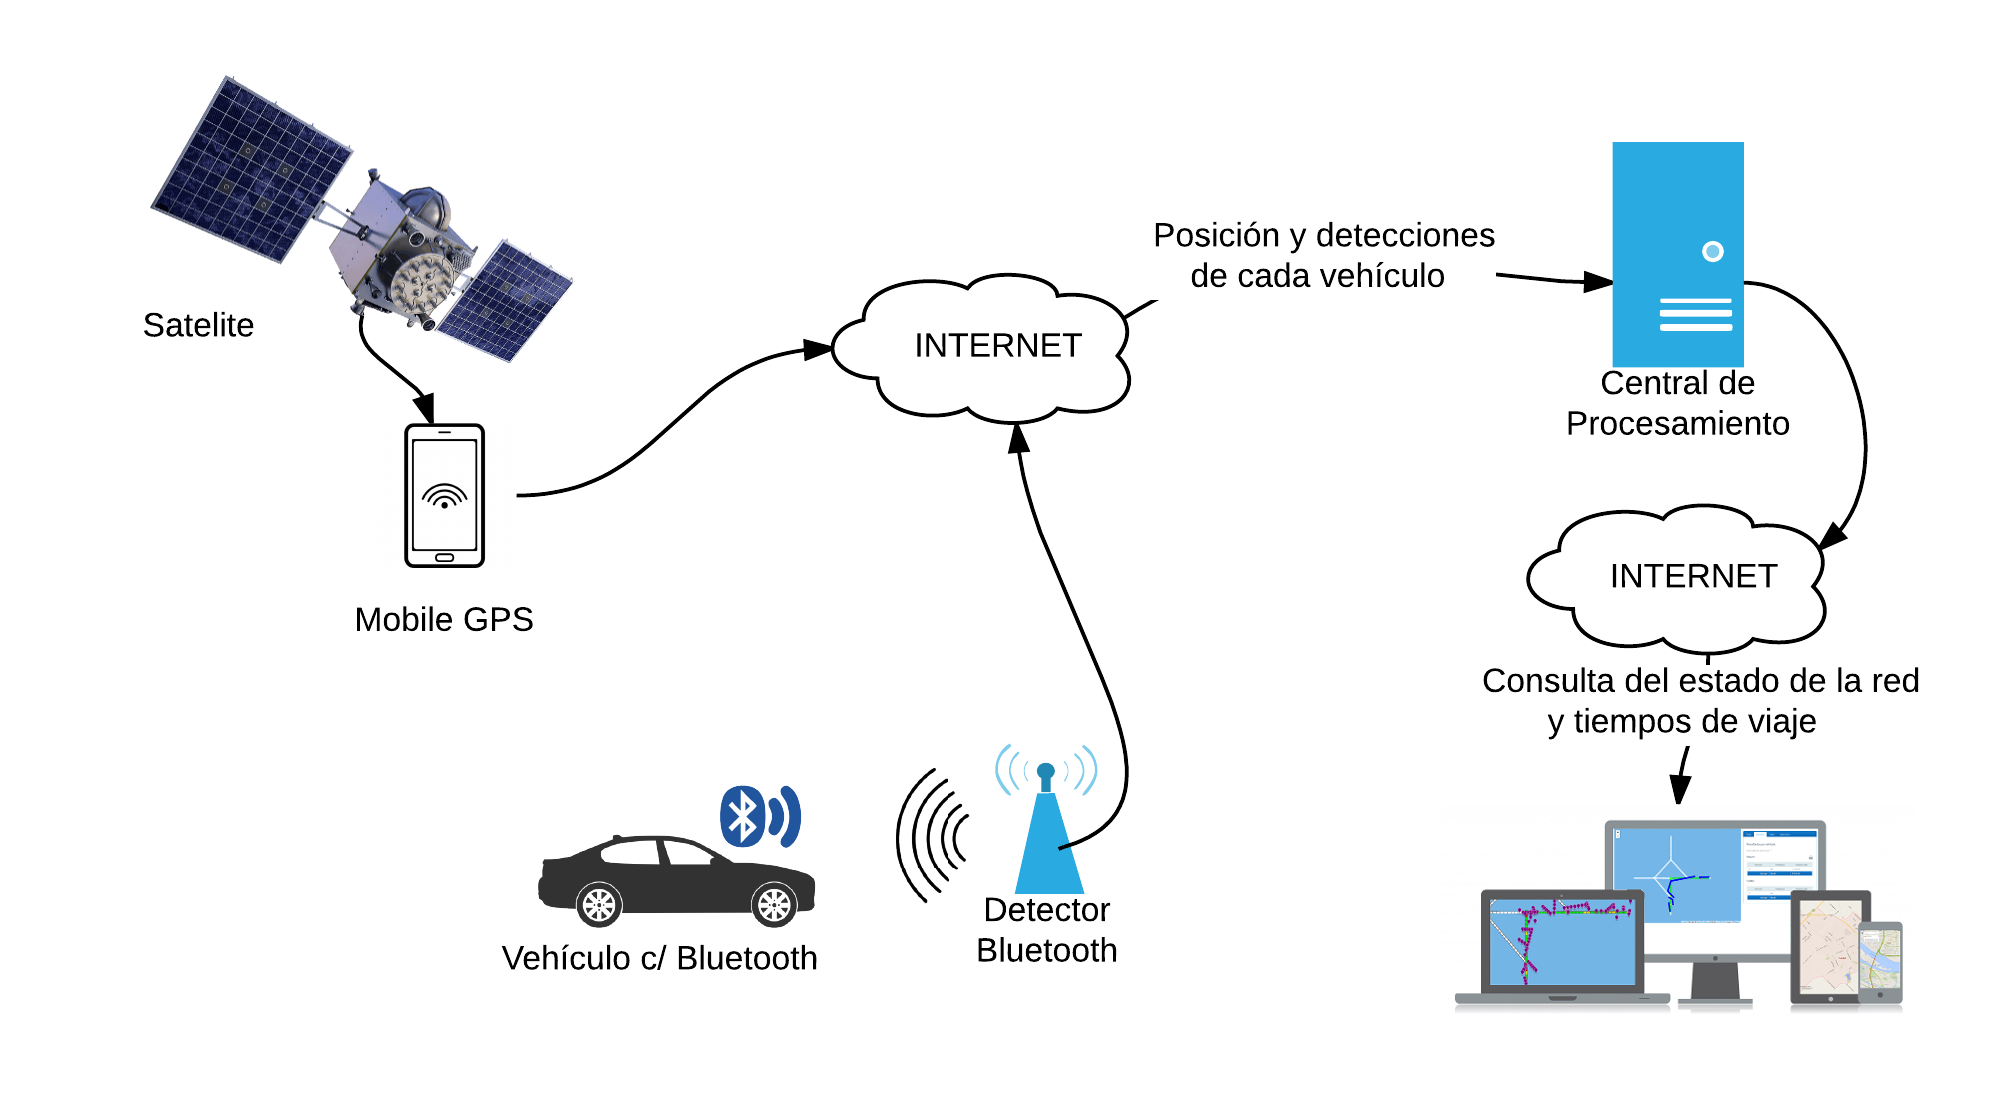
\includegraphics[scale=0.9]{images/deployment.png}
	\caption{Diagrama de despliegue}
    \label{fig:deployment}
\end{figure}

Para facilitar el envío de datos al centro de procesamiento, se implementó una capa de servicios web que incluye interfaces para el almacenamiento y recuperación de lecturas GPS y Bluetooth.

\subsection{Arquitectura propuesta para un sistema de estimación de tráfico vehicular}

En la primera iteración de la etapa de diseño, se decidió mantener dos módulos ``SumoUtils'' y ``Viterbi''  (Figura \ref{fig:modulos-gral}) para las tareas de simulación y estimación, respectivamente. Complementariamente, se desarrolló un tercer módulo de persistencia de datos ``Monitores.WS''. Éstos fueron separados para independizar la simulación (creación de datos) y almacenamiento de detecciones de los algoritmos de estimación. 

\begin{figure}[!htp]
	\centering
	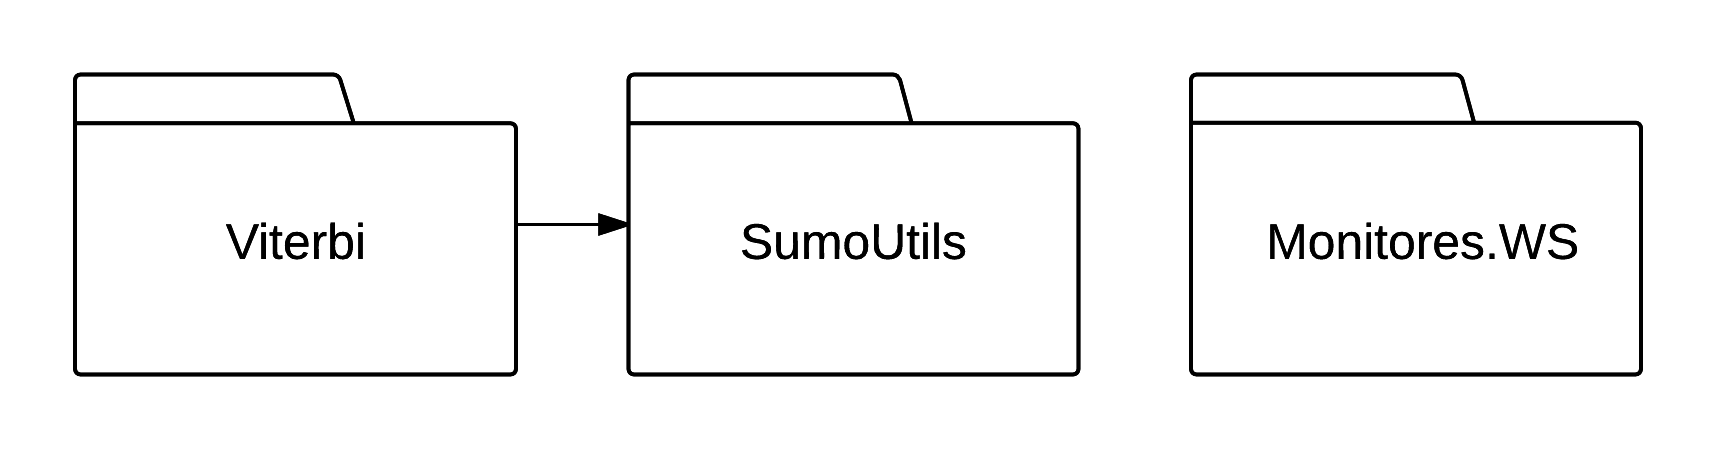
\includegraphics[scale=0.8]{images/modulos-gral.png}
	\caption{Vista de módulos principales del sistema}
    \label{fig:modulos-gral}
\end{figure}

La división de los módulos favorece el bajo acoplamiento ya que se reduce la dependencia directa entre las partes. Por esto, es posible alternar las fuentes de origen de datos entre observaciones reales y datos simulados a muy bajo costo de desarrollo. La dependencia del módulo \textit{Viterbi} con \textit{SumoUtils} se debe a que el estimador es una herramienta completa con soporte para configurar y ejecutar simulaciones.

Acorde al plan de trabajo, el módulo \textit{Viterbi} fue el primero en desarrollarse. Para contar con datos de prueba en etapas tempranas del proyecto, se adelantó la implementación del módulo de simulación \textit{SumoUtils}.  

\section{Simulación de tráfico}

En general, la simulación se define como una representación dinámica de una parte del mundo real, lograda con la construcción de un modelo computacional, evolucionado a lo largo del tiempo. El modelado y simulación (M\&S) es la herramienta de preferencia para explorar los problemas de transporte\cite{sokolowski2011principles}. Provee un método efectivo a bajo costo para solucionar problemas sin poner en riesgo al público o invirtiendo en construcción sin fundamentos. Es ampliamente utilizado en el área de transporte terrestre (caminos, rutas y autopistas). Dos problemas clásicos donde se utiliza M\&S son:

\begin{itemize}
    \item \textit{Planificación de transporte:} Los problemas de planificación de transporte están centrados en pronosticar condiciones de tráfico a futuro, típicamente entre 10 y 20 años desde el presente. Estos análisis generalmente tienen un alcance regional. Un ejemplo de estos problemas es predecir si la extensión de carriles de una autopista solucionaría problemas de congestión a 20 años. Modelos macroscópicos se utilizan para evaluar estos casos.
    \item \textit{Problemas operacionales de transporte:} La idea principal es crear un análisis detallado de problemas a escalas pequeñas, como calles individuales o intersecciones. Por ejemplo, determinar cuánto tiempo debe darse luz verde en una señal de tráfico para reducir la congestión. Modelos microscópicos se utilizan en este caso.
\end{itemize}

\subsection{Modelos de simulación de tráfico}

Los modelos de simulación están clasificados de acuerdo al nivel de detalle al cual representan el flujo de tráfico. Estos incluyen:

\begin{description}
    \item [Modelo macroscópico:]
    El modelado macroscópico del flujo del tráfico está basado en la teoría de flujo de tráfico contínuo, cuyo objetivo es la descripción de la evolución espacio-temporal de las variables que caracterizan los flujos macroscópicos: volumen,  velocidad, y densidad, sobre las cuales se asume que están definidas en cada instante de tiempo $t$ y cada punto $x$ en el espacio\cite{barcelo2010fundamentals}. 
    \item [Modelo microscópico:] Estos modelos simulan las características e interacciones entre vehículos individuales. Esencialmente, producen trayectorias de los vehículos mientras se trasladan a través de la red. La lógica de procesamiento incluye algoritmos y reglas que describen cómo se mueven e interactúan los vehículos, incluyendo aceleración, desaceleración, cambio de carril y maniobras de adelantamiento.
\end{description}

Los modelos microscópicos son más precisos que los modelos de simulación macroscópicos. Sin embargo, emplean más parámetros que requieren calibración. De este modo, los parámetros de los modelos macroscópicos (ej. capacidad) son observables en el escenario real. Por otro lado, la mayoría de los parámetros de los modelos microscópicos no pueden ser observados directamente en la zona (ej. distancias mínimas entre vehículos)\cite{dowling2004traffic}.

Dentro de los modelos microscópicos, por cada vehículo en la red se generan características del conductor, como grado de tolerancia a las distancias, velocidad deseada y agresividad en aceleración y frenado. Usar simulación posibilita tener en consideración variables aleatorias del mundo real al momento de realizar estudios de tráfico.

El modelo microscópico se ajusta a las necesidades del proyecto. En particular, la posibilidad de simular cada vehículo individualmente lo convierte en el modelo ideal para la generación de observaciones.

 \begin{figure}[!htp]
	\centering
	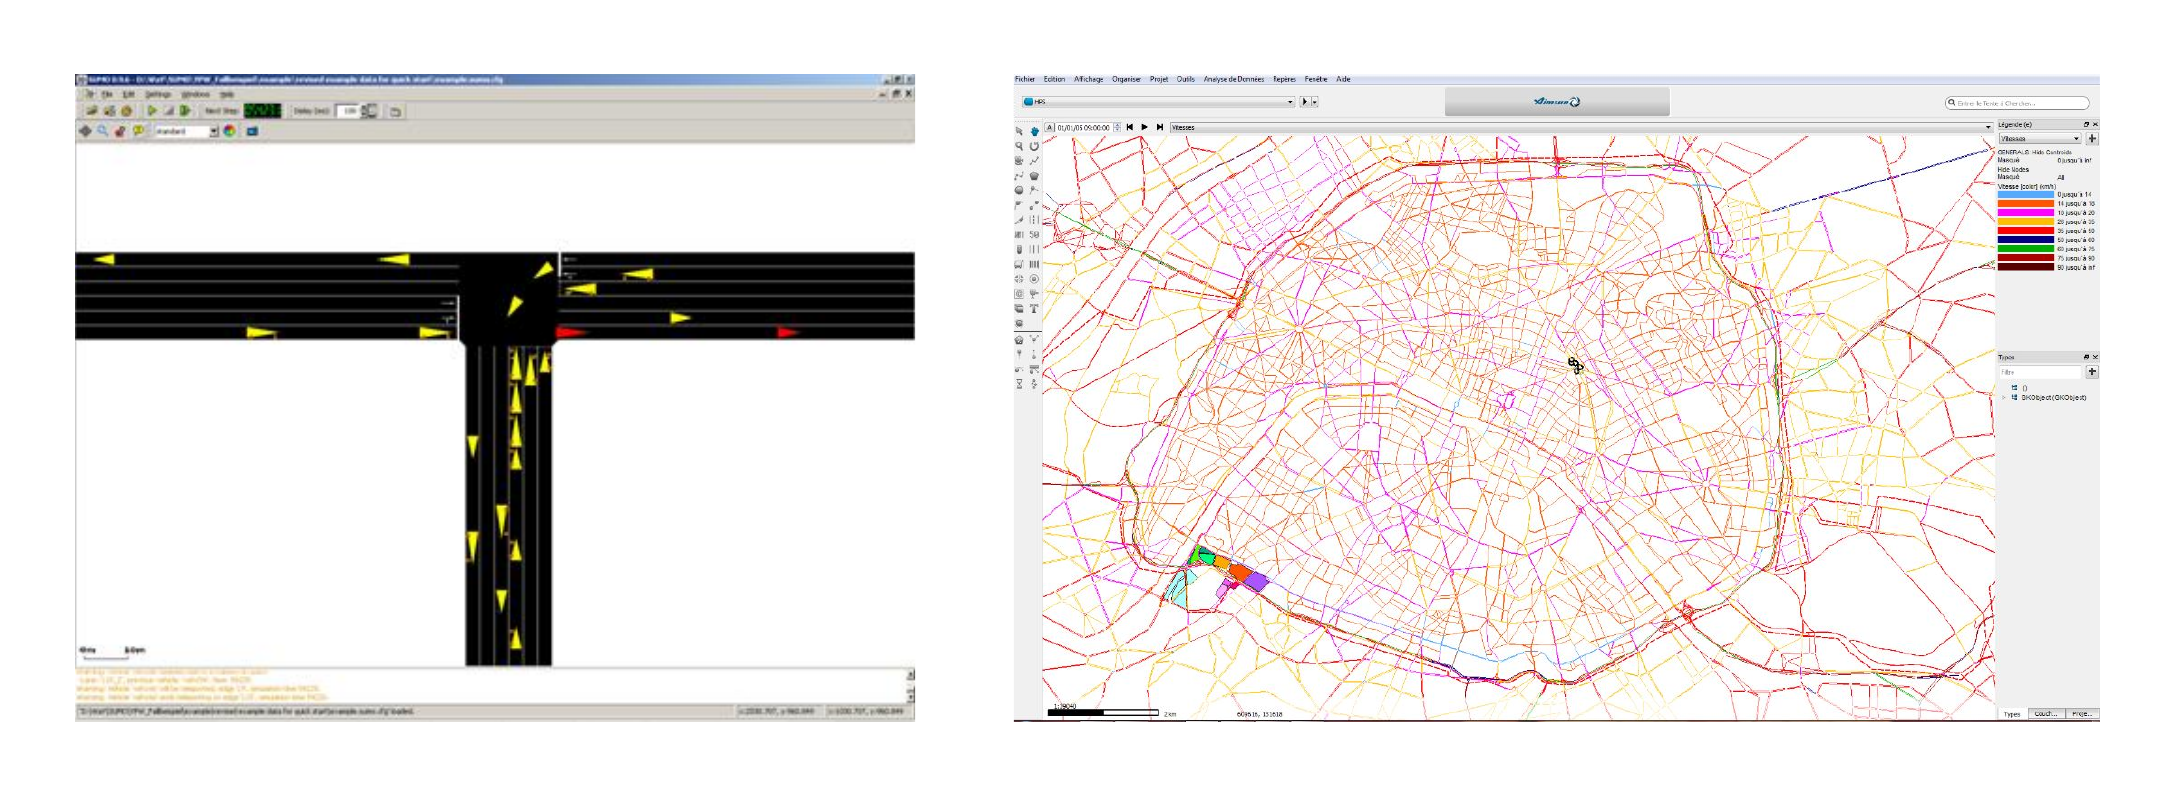
\includegraphics[width=0.9\textwidth]{images/sumo-aimsun.png}
	\caption{Simulación microscópica en SUMO (izq). Simulación macroscópica en AIMSUN}
    \label{fig:sumo-aimsun}
\end{figure}

Existen múltiples herramientas de micro-simulación, entre las que se encuentran SUMO (Simulation of Urban MObility) y AIMSUN (Figura \ref{fig:sumo-aimsun}) \cite{ronaldo2012comparison}. AIMSUN es una solución comercial, ampliamente utilizada, que se destaca por la velocidad excepcional de sus simulaciones. También soporta simulación macroscópica.  SUMO es una alternativa no comercial, desarrollada por el Instituto de Sistemas de Transporte en el Centro Aeroespacial Alemán. En el trabajo actual, se optó por la herramienta SUMO.

\subsection{SUMO}

SUMO está construido para simular una red de tráfico del tamaño de una ciudad. El simulador es multi-modal, lo cual significa que no solo se modelan los movimientos de los vehículos, también se modelan los sistemas de transporte público, como por ejemplo, recorridos alternativos de trenes. Concebido como una herramienta para investigadores, está diseñado para ser rápido y exacto en lugar de ser un software agradable a la vista. Está implementado en el lenguaje C++, en su mayoría haciendo uso de partes estandarizadas del lenguaje, como la biblioteca STL, para maximizar la portabilidad.

En la herramienta, hay 4 pasos necesarios para realizar una simulación:

\subsubsection*{Construcción de la red}
    Un archivo de red SUMO describe la parte del mapa relacionada con tráfico. Contiene la red de caminos, carriles, intersecciones y semáforos. Para construir una red SUMO (Figura \ref{fig:sumonet}), es posible generar una red abstracta con el submódulo NETGEN, detallando una descripción específica en XML e importarla utilizando NETCONVERT; o bien, importando una red existente a través de NETCONVERT. Los mapas importados pueden provenir de redes ajenas a SUMO, como OpenStreetMap, VISUM, ArcView, entre otras. A pesar de las características reales que incluye una red importada, SUMO aún puede requerir algunos ajustes para representar las condición exacta deseada. En la traducción a redes SUMO, el mapa es trasladado al origen de coordenadas del plano cartesiano $(0;0)$, situando la red en el primer cuadrante.
    \begin{figure}[!htp]
    	\centering
    	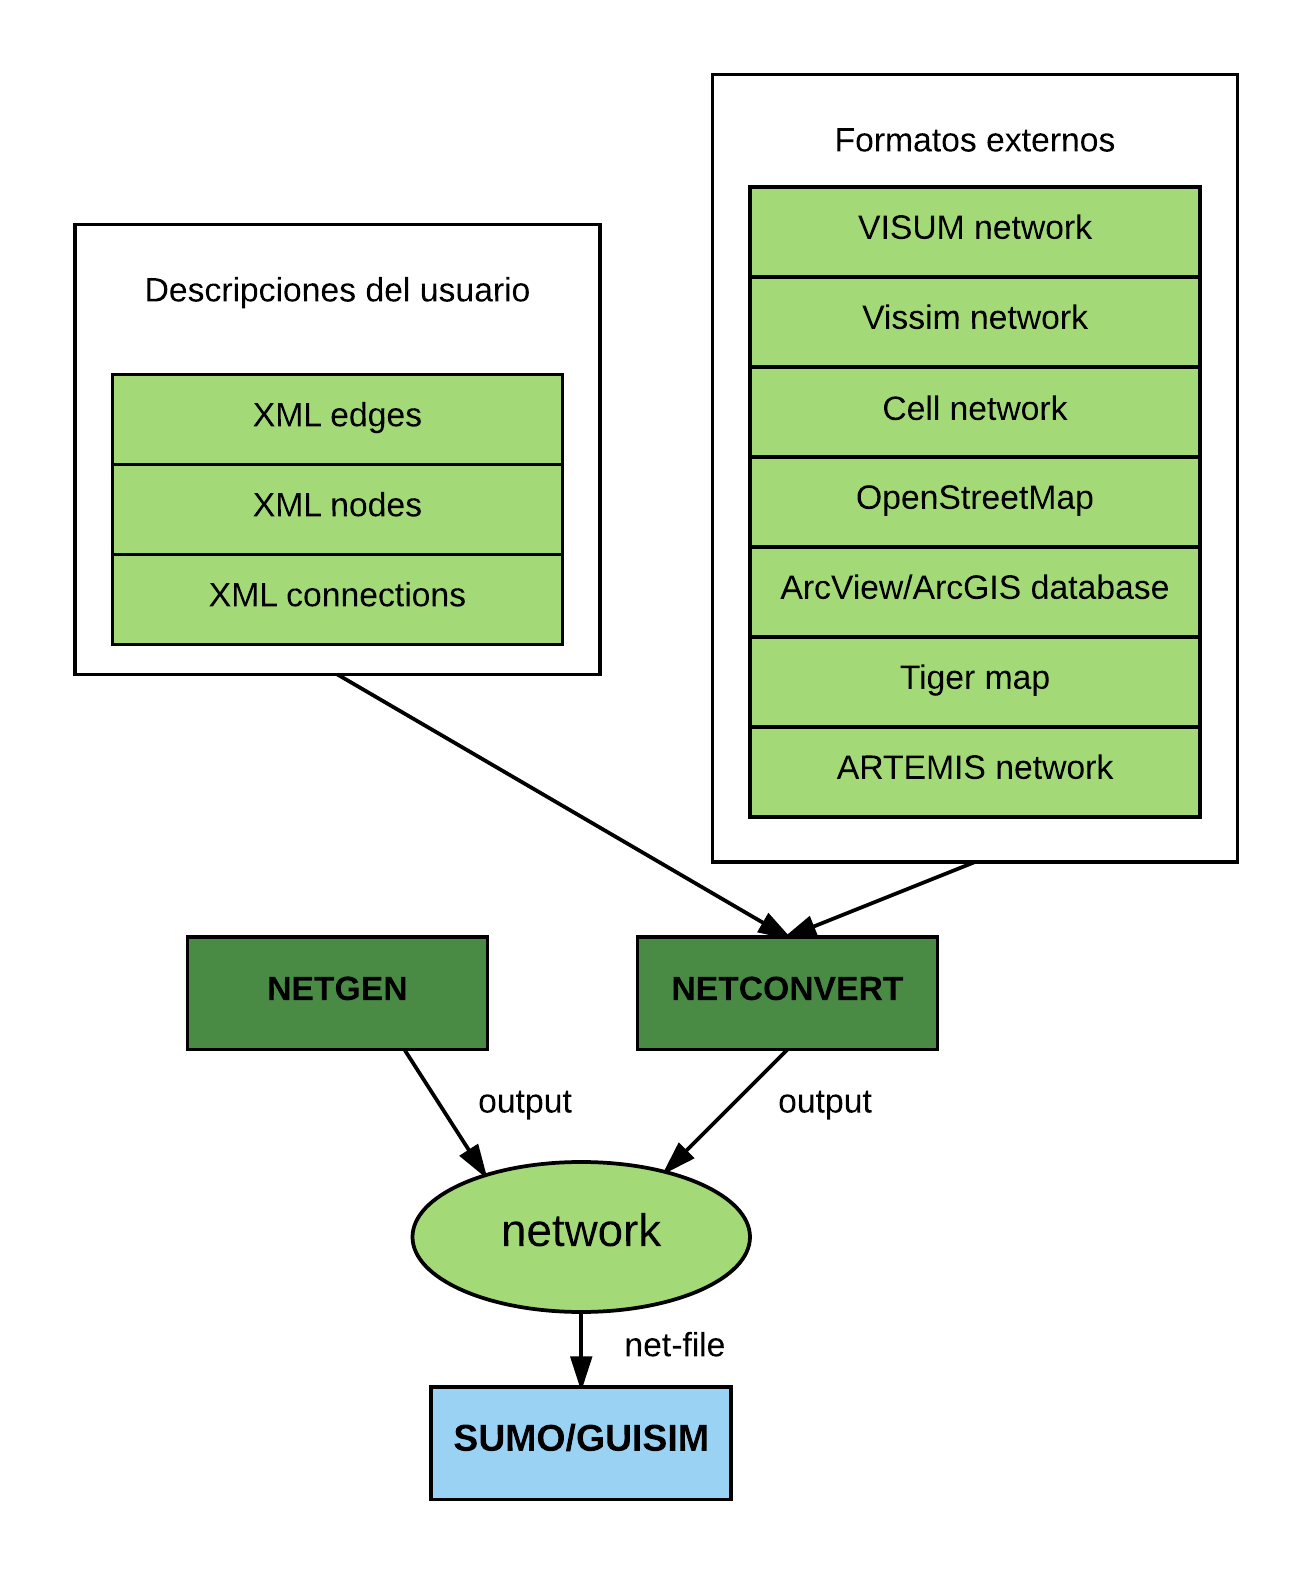
\includegraphics[scale=0.6]{images/sumo-buildnet.png}
    	\caption{Construcción de una red SUMO}
        \label{fig:sumonet}
    \end{figure}

\subsubsection*{Definición de la demanda}
    Una vez construida la red, se deben establecer los flujos de tráfico dentro de la misma. Para esto, la herramienta incluye diversos métodos: generación explícita de recorridos, generación a partir de definiciones de flujos y tasas de giro, e importación de matrices Origen-Destino (OD) pre-existentes. Las matrices OD deben ser procesadas para obtener los recorridos (SUMO soporta importación de recorridos en formatos VISUM/VISION/VISSIM). Es posible convertir matrices al formato especificado con el submódulo OD2TRIPS, en el caso de no tener matrices compatibles (Figura \ref{fig:sumodemand}). Finalmente, se obtienen los recorridos a partir de la demanda con la herramienta DUAROUTER, en la cual se aplican algoritmos de caminos mas cortos para conectar la demanda. 
    \begin{figure}[!htp]
    	\centering
    	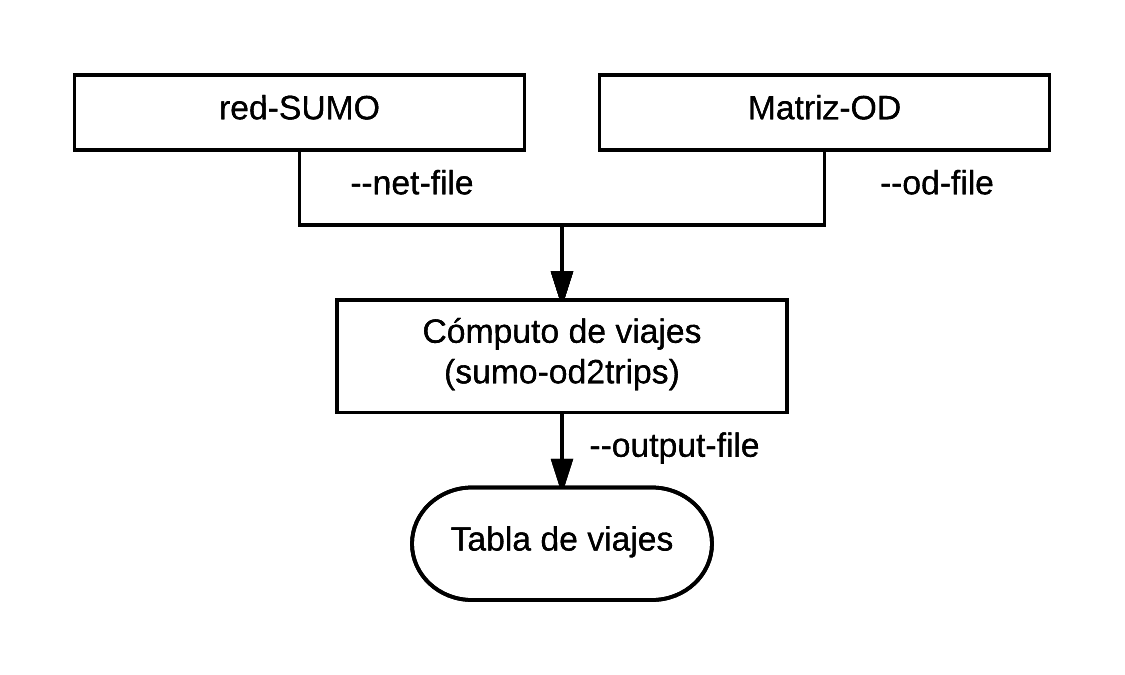
\includegraphics[scale=0.7]{images/sumo-builddemand.png}
    	\caption{Definición de la demanda en SUMO}
        \label{fig:sumodemand}
    \end{figure}
    
\subsubsection*{Asignación dinámica de rutas (opcional)}
    Se busca calcular el equilibrio del usuario, esto es, intenta buscar un recorrido para cada vehículo tal que cada vehículo no pueda reducir su tiempo de viaje usando una ruta distinta. Se aplica de forma iterativa en 2 pasos: DUAROUTER enruta nuevamente a los vehículos en una red con los últimos costos de cada arco conocidos (comenzando con el tiempo de viaje de la red vacía). Luego, SUMO realiza una simulación para obtener el tiempo de viaje real del recorrido calculado en el paso previo.
    
\subsubsection*{Ejecución de la simulación}
   El archivo de la red, la información de recorridos que serán utilizados y el período de tiempo de la simulación son necesarios para iniciar el modelo.
    
\subsection{SumoConvert}

Originalmente, SUMO se distribuye como un conjunto de herramientas que deben ser utilizadas individualmente para su funcionamiento. Como se mencionó en el capítulo introductorio, este trabajo surge como parte de un proyecto mayor alcance. En una instancia anterior, se desarrolló un \textit{plugin} (una extensión) para el editor de mapas JOSM (de OpenStreetMap), llamado ``SumoConvert''. Esta extensión incluye características que facilitan el trabajo con el simulador. Las funcionalidades utilizadas de este trabajo son:
\begin{itemize}
    \item Traducción de mapas de la plataforma OpenStreetMap a mapas soportados por 'SUMO' (net-files).
    \item Definición de distritos (zonas para modelar la demanda).
    \item Asignación de la demanda y períodos de tiempo (Matrices OD).
    \item Despliegue de detectores inalámbricos (AccessPoints/APs) sobre la red
    \item Exportación de datos de simulación en archivos de texto plano CSV (Comma separated values) 
\end{itemize}

 \begin{figure}[!htp]
	\centering
	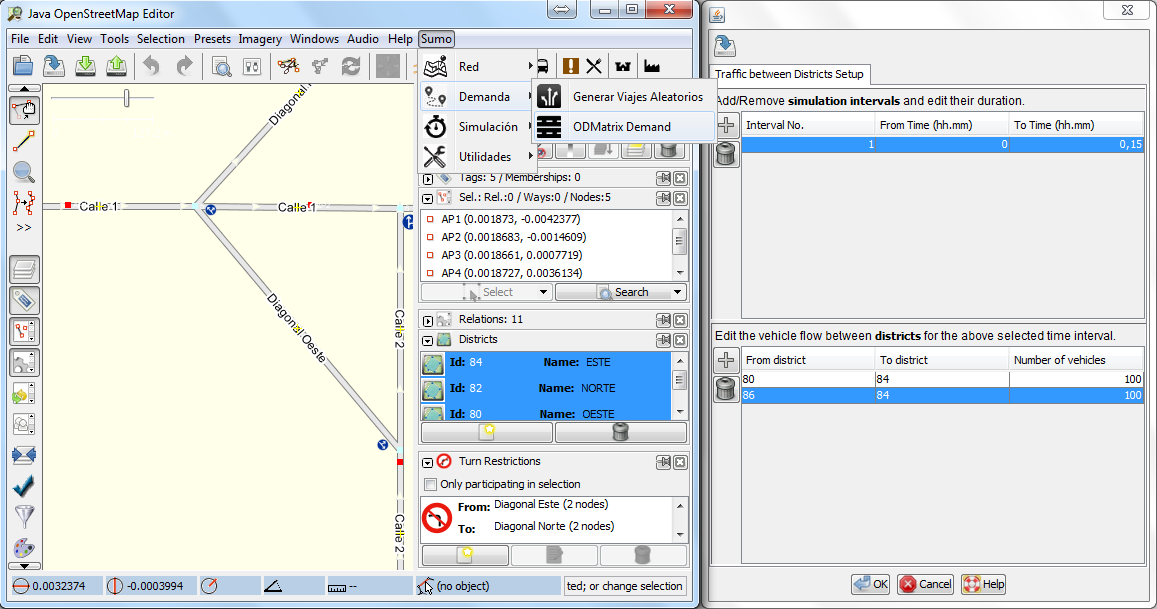
\includegraphics[width=0.9\textwidth]{images/osm2sumo.png}
	\caption{Extensión de JOSM: 'SumoConvert'}
    \label{fig:sumoconvert}
\end{figure}
    
Finalmente, ``SumoConvert'' integra las herramientas de SUMO para realizar la conversión y generación de viajes desde el mismo editor de mapas (Figura \ref{fig:sumoconvert}).

Recuperar información de una simulación en ejecución es posible desde la herramienta ``TraCI'' (Traffic Control Interface), una interfaz de acceso a una simulación en tiempo real. Desde \textit{TraCI} es posible obtener datos del estado de cada vehículo en cada tiempo de simulación y, de este modo, se escriben valores seleccionados en archivos de texto plano. Entre los archivos generados por cada simulación, en este trabajo se utilizan:

\begin{description}
    \item [Smartphone detections:] Las detecciones de smartphones simulan sensores GPS equipados por los vehículos. Cada detección incluye: ciclo de simulación (tiempo $t$), identificación del vehículo, posición $x$, posición $y$, velocidad y el arco donde se encontraba el vehículo en el mismo instante $t$ (edge). Las posiciones registradas son relativas al sistema de coordenadas del simulador. Por lo tanto, las posiciones deberán ser trasladas nuevamente al sistema de coordenadas del mapa original.
    \item [Bluetooth detections:] Se registran detecciones por los AP desplegados en la red de sólo algunos vehículos. Se determinan aquellos vehículos que cuentan con dispositivos inalámbricos a partir de la probabilidad de penetración, ingresada desde la herramienta. Las detecciones de APs incluyen: ciclo de simulación, identificación del AP que realizó la detección, identificación del dispositivo/vehículo y la distancia del AP al vehículo (en el momento de la detección). El cálculo de la potencia de señal recibida se pospone para la aplicación de dos métodos diferentes, introducidos en la sección \ref{ssec:modulo-sim}.
\end{description}

\section{Paquete de utilidades para SUMO-SumoConvert}\label{ssec:modulo-sim}

El módulo SumoUtils, dedicado principalmente al procesamiento de simulaciones, complementa la solución ``SUMO-SumoConvert''. En las próximas secciones se describe la metodología utilizada para ajustar observaciones GPS y realizar simulaciones de la potencia de señal recibida de dispositivos Bluetooth sobre simulaciones SUMO. Adicionalmente, se agregan funcionalidades para la persistencia de los mapas a la plataforma.


\begin{figure}[!htp]
	\centering
	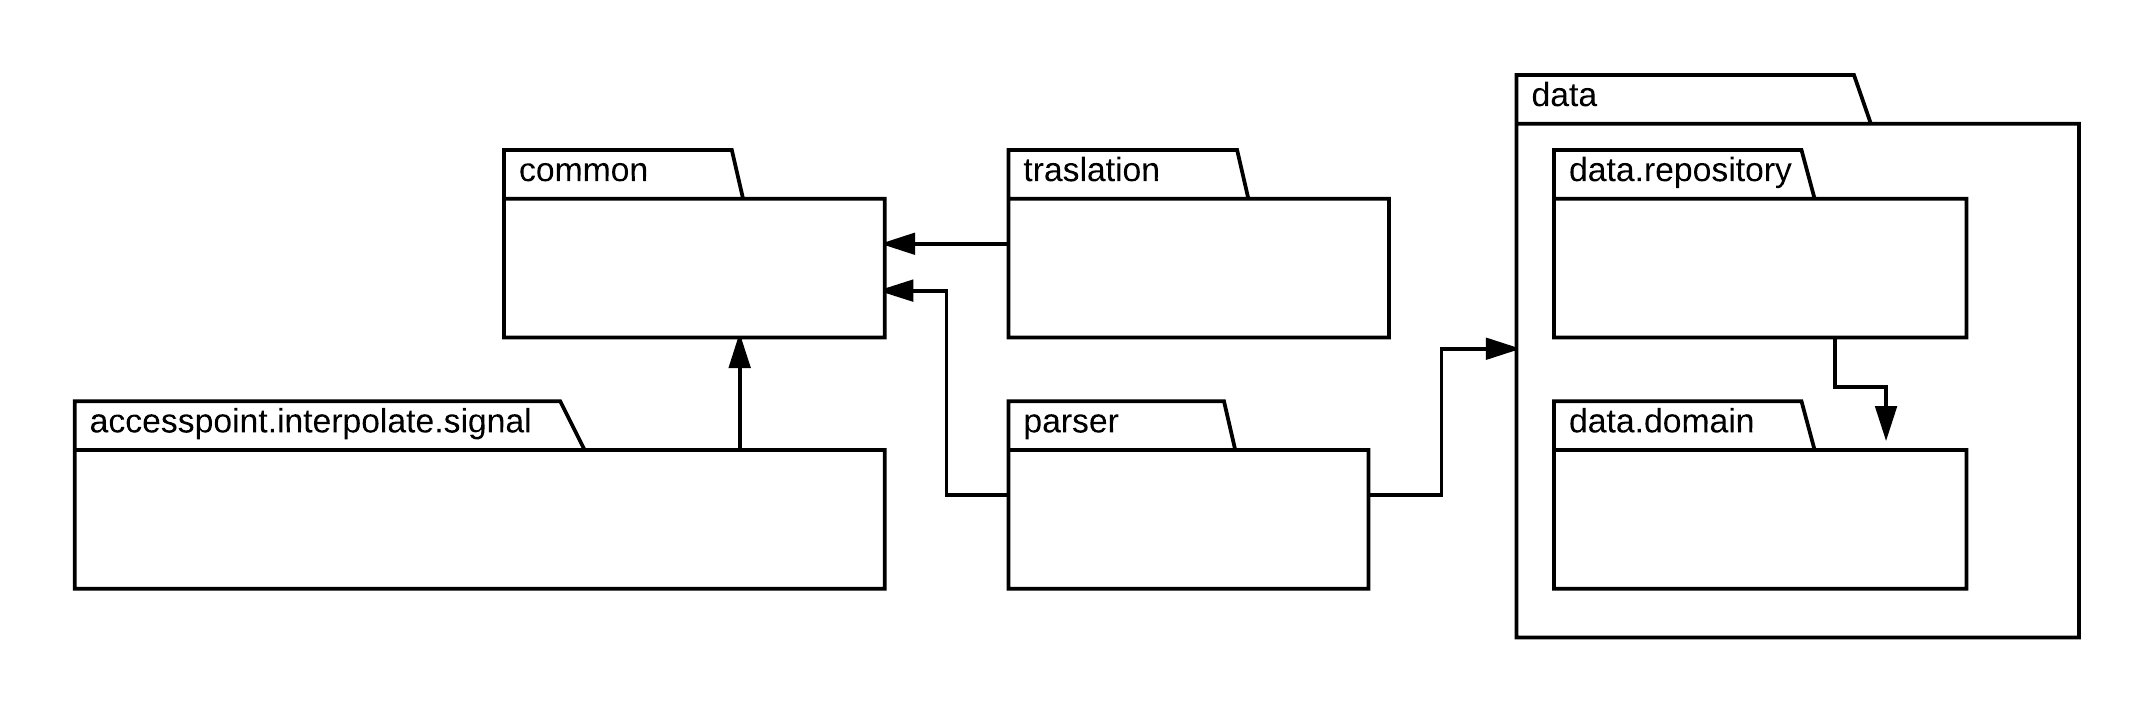
\includegraphics[width=\textwidth]{images/simulacion-general.png}
	\caption{Vista de módulos - SumoUtils}
    \label{fig:modulos-sim}
\end{figure}

\subsection{Simulación GPS}

Como se describió en el apartado anterior, las observaciones generadas en ``Smartphone detections'' deben ser trasladadas nuevamente al sistema de coordenadas del mapa original. Para realizar este post-procesamiento se utiliza el archivo de red net.xml, el cual almacena el ajuste (offset) aplicado para trasladar la red al origen de coordenadas. A partir del offset se realiza la conversión en 2 pasos, para cada observación:

\begin{enumerate}
    \item Normalización: Dada una observación $p=(x;y)$ y los límites de convolución de la red simulada $L_S=(x_0;y_0;x_1;y_1)$, se calcula el punto relativo al sistema de coordenadas de la simulación en el rango de normalización [0,1]. Por ejemplo, dado un límite de convolución  $L_S={0;0;2;2}$ y un punto $p_0 = (1;1)$, la normalización obtiene un punto $p_n = (0.5;0.5)$
    \item Traslación: Dado un punto normalizado $p_n$ y el límite de convolución del mapa original $L_{O}$, se mapea $p_n$ al sistema de coordenadas del mapa original. Por ejemplo, se mapea el punto $p_n = (0.5;0.5)$ a $L_{O}={-10;-10;-5;-5}$, dando como resultado el punto en el sistema original $p_O=(-7.5;-7.5)$.
\end{enumerate}

 
\subsection{Simulación Bluetooth} \label{ssec:bt-simulation}
Un vehículo será detectado por un sensor si la potencia de las antenas de transmisión y recepción, y el dispositivo en el vehículo satisfacen la ecuación de transmisión de Friis (Ecuación \ref{eq:friis}). Si se dan las condiciones ideales, a partir de las especificaciones del dispositivo Ubertooth One (sensor) se determina la distancia de cobertura como $d \approx 100$ m (Bluetooth Clase 1). La FHWA (Federal Highway Administration - Estados Unidos) sugiere un tamaño de carril de 3.6 m de ancho para rutas, 3.3 m para arterias principales y 2.7 m para calles internas. Si se asume que el ancho de un carril es de 3.2 m y los detectores se ubican sobre el camino, la probabilidad de detección en condiciones ideales es de 100\%, cubriendo el tráfico en ambas direcciones.

Se determina entonces la distancia a la que se observaría a un dispositivo en viaje desde cada detector, si este hiciese alguna transmisión. De este modo, cada monitor registra la distancia del vehículo al detector, sólo si éste se encuentra dentro del área de cobertura. Se consideran antenas isotrópicas en todos los casos, es decir, antenas que irradian el haz de la señal en todas las direcciones (en un plano horizontal).

Obtenida la distancia de los vehículos en los distintos tiempos de simulación, es necesario traducir el valor de distancia a una intensidad de señal. La traducción se realiza a través de dos métodos propuestos en este trabajo. Los métodos surgen del procesamiento de las lecturas obtenidas por experimentación, introducidas en la sección \ref{sec:estimacionwireless}. A continuación se detalla el diseño de las pruebas de campo y posteriormente las características de los métodos de simulación.

\begin{figure}[!htp]
	\centering
	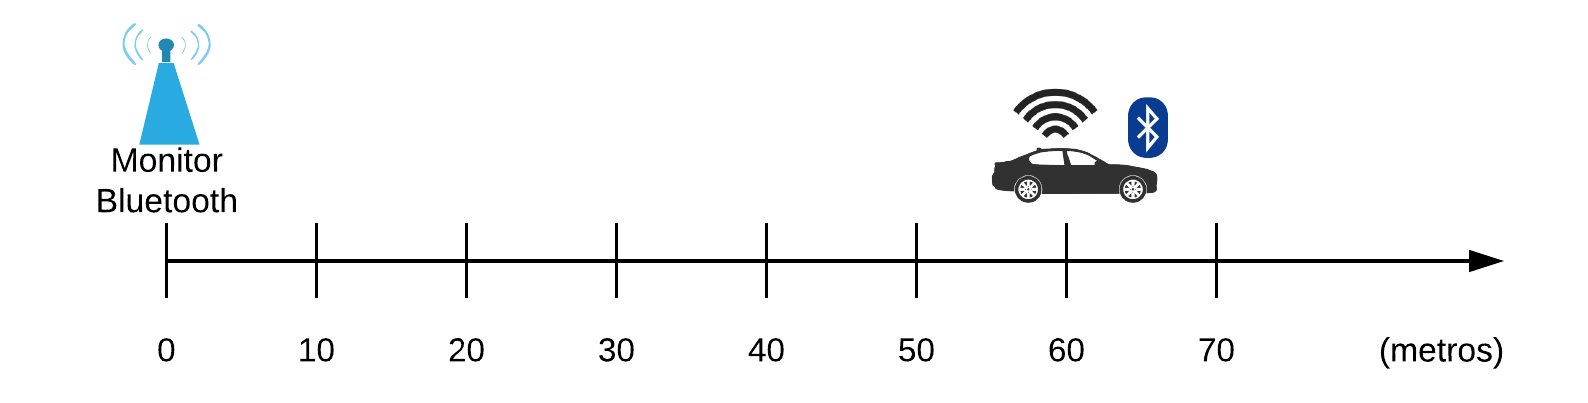
\includegraphics[width=\textwidth]{images/bt-experiment.png}
	\caption{Diseño de pruebas Bluetooth}
    \label{fig:opdf-experiment}
\end{figure}

El experimento fue diseñado con el fin de registrar la intensidad de señal y la distancia de los paquetes transmitidos al conducir a lo largo del alcance de un monitor con un dispositivo BT activo. El vehículo utilizado cuenta con un sistema de sonido Bluetooth. A partir de éste se generan las transmisiones recolectadas. Se aislaron los equipos de transmisiones no controladas realizando las medidas en una zona de escasa población, con edificación y actividad vehicular nula (Figura \ref{fig:pruebas-empiricas}).

Mediciones preliminares indicaron un alcance máximo de 80 mts sobre el rango de detección del monitor, con baja cantidad de paquetes observados. Dado el indicador, se diseñó el siguiente procedimiento para la medición: desde una distancia próxima al detector y durante intervalos de 1 minuto, se debe registrar la distancia y los valores de señal de los paquetes transmitidos. Luego de cada intervalo de detección, el vehículo avanza en dirección opuesta al detector, según el esquema de distancias representado por la Figura \ref{fig:opdf-experiment}. De este modo, se obtienen lecturas de transmisiones de señal clasificadas por distancia. Estos datos aportan una idea aproximada de qué valores de señal se transmiten a qué distancia.

\begin{figure}[!htp]
	\centering
	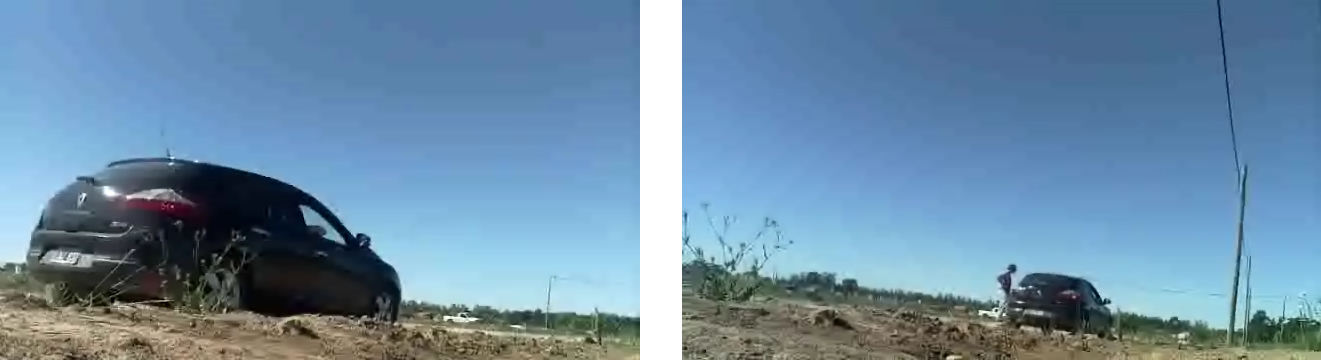
\includegraphics[width=\textwidth]{images/pruebas-empiricas.png}
	\caption{Imágenes del registro videográfico del experimento a distancias de 5 y 15 metros, respectivamente. Capturado desde la cámara presente en la caja ``Sensor''.}
    \label{fig:pruebas-empiricas}
\end{figure}

Se consideró aplicar un filtro sobre valores atípicos (outliers) debido a la alta dispersión de las muestras recolectadas. Para remover cierto porcentaje $p_{outlier}$ de valores atípicos se utilizó el componente \textit{DescriptiveStatistics} de la biblioteca Apache Commons Math. \textit{DescriptiveStatistics} permite obtener una estimación del p-ésimo percentil (escalado de 0-100) de un arreglo de datos: getPercentile($p_{outlier}$). De este modo se excluyen del dataset los valores de señal $s$ tales que $s < getPercentile(p_{outlier})$ y $s > getPercentile(1-p_{outlier})$. Para las pruebas realizadas, se utlizaron los siguientes porcentajes de eliminación de outliers:

\begin{itemize}
    \item $p_{outlier}=0.02$ (2\% sobre el total de la muestra)
    \item $p_{outlier}=0.05$ (5\% sobre el total de la muestra)
    \item $p_{outlier}=0.10$ (10\% sobre el total de la muestra)
    \item $p_{outlier}=0.20$ (20\% sobre el total de la muestra)
\end{itemize}

Además, se consideró aplicar el filtro a toda la muestra y a los valores agrupados por distancia. 
\begin{figure}[!htp]
	\centering
	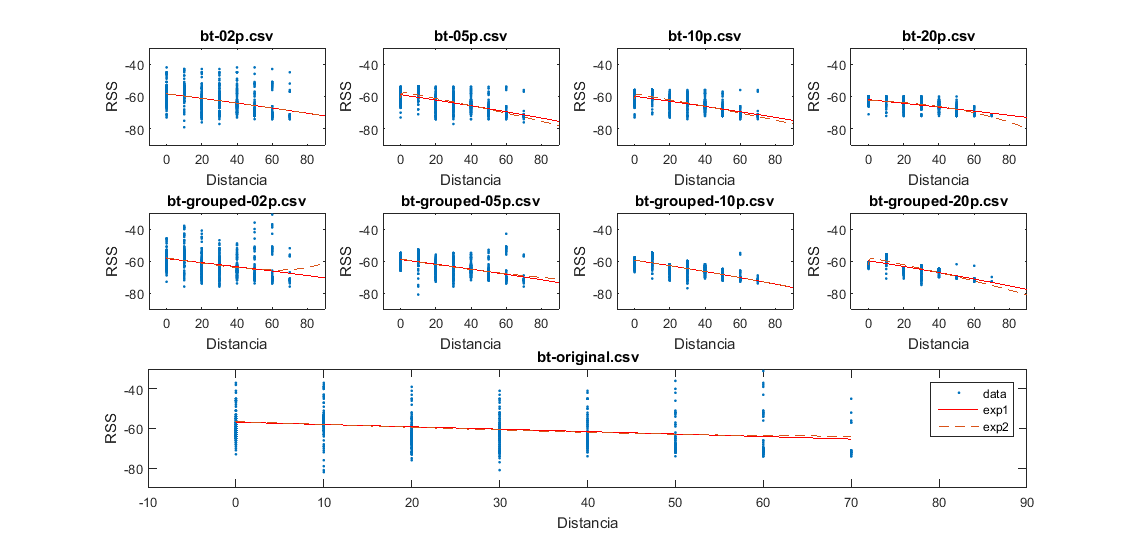
\includegraphics[width=\textwidth]{images/distancia_rss.png}
	\caption{Conjunto de datos recolectados via sensor Bluetooth}
    \label{fig:datos-bluetooth}
\end{figure}

Para agilizar el análisis de los grupos, se realizó el mismo procesamiento en Matlab. Esta herramienta permite realizar gráficos  de los datos de un arreglo sencillamente con el comando \textit{plot(Y)}, o bien, \textit{plot(X,Y)} si se cuenta con los correspondientes valores del eje horizontal.

Los métodos desarrollados para obtener valores de señal a partir de la distancia detectada por el simulador abarcan dos técnicas considerablemente diferentes. El primer conjunto de datos se genera utilizando la ecuación (\ref{eq:regresion_bluetooth}), obtenida por regresión exponencial sobre el conjunto de medidas experimentales descrito previamente (Figura \ref{fig:datos-bluetooth}). Se obtiene entonces una intensidad de señal a partir de la distancia del vehículo al detector, registrada por el simulador.
\begin{align}\label{eq:regresion_bluetooth}
 signal = -62.85 * e^{0.001936*d}
\end{align}

 A modo de ejemplo, en el cuadro \ref{tbl:bluetooth-data} se observan los elementos correspondientes a una detección Bluetooth, calculando la potencia de señal utilizando la ecuación \ref{eq:regresion_bluetooth}. Cabe aclarar que para cada valor de distancia, corresponde un único valor de señal.

\begin{table}[h]
\centering
\begin{tabular}{|c|c|c|c|c|}
\hline
Tiempo & Monitor & Vehiculo & Distancia(m) & Señal (dB)\\
\hline
401 & AP1 & 349e4a & 23.85 & -65.82\\
\hline
\end{tabular}
\caption{Ejemplo de simulación: detección Bluetooth}
\label{tbl:bluetooth-data}
\end{table}

Respecto a los datos simulados, es deseable contar con el error inherente a los dispositivos Bluetooth. Si bien es sabido que el error mencionado no sigue una distribución normal, éstas son ampliamente utilizadas en estudios de investigación por los buenos resultados que ofrecen\cite{cinefra2014adaptive}. Se introduce entonces el error a través de una aleatorización basada en distribuciones normales, con medias y desvíos que dependen de la distancia de la detección: Dada una distancia $d$, se asocia una distribución normal con media $\mu(d)$ y desvío $\sigma(d)$, calculadas por interpolación (Ecuación \ref{eq:linear_interpolation}) sobre las medias y desvíos registrados (Figura \ref{fig:medias-desvios}). Para cada distancia registrada se obtienen valores aleatorios según la distribución.

\begin{figure}[!htp]
	\centering
	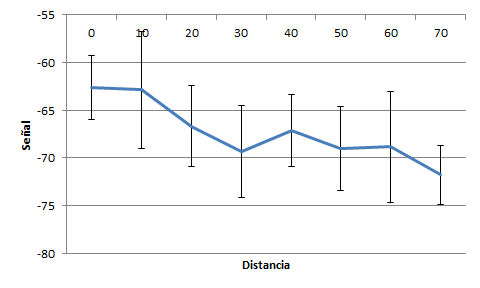
\includegraphics[scale=0.35]{images/medias_y_desvios.png}
	\captionsetup{width=0.6\textwidth}
	\caption{Señal media y desvío estándar de las muestras experimentales según la distancia al monitor}
    \label{fig:medias-desvios}
\end{figure}

\begin{equation}\label{eq:linear_interpolation}
y_2=\frac{(x_2-x_1)(y_3-y_1)}{x_3-x_1}+y_1
\end{equation}

El paquete \textit{sumoutils.accesspoint.interpolate.signal} posee un procesador de archivos separados por coma (CSV) para leer los valores medios y desvíos registrados experimentalmente. Estos valores son utilizados para construir distribuciones normales. Se utiliza el componente \textit{NormalDistribution} de la biblioteca Apache Commons Math3 para generar valores aleatorios de esta distribución. El algoritmo \ref{alg:perturbate} genera un valor aleatorio en una distribución dada por la distancia de una detección realizada en SUMO.

\clearpage

\begin{lstlisting}[language=Java, caption=Perturbación de detecciones Bluetooth, label=alg:perturbate]
[signal] perturbate(Detection det) {
	dev = desviosPorDistancia.get(det.getDistance().intValue());
	NormalDistribution gaussian = new NormalDistribution(dev.getMean(),
				dev.getDeviation());
	return gaussian.sample();
}
\end{lstlisting}

A modo de ejemplo, se ilustran en la Figura \ref{fig:eq-vs-means} las potencias de señal generadas para una simulación de un vehículo atravesando el área de detección de 4 monitores. En la curva del método por ecuación (azul) se logran identificar los momentos mas próximos a cada detector (tiempos 67, 93, 116 y 141 aproximadamente).

\begin{figure}[!htp]
	\centering
	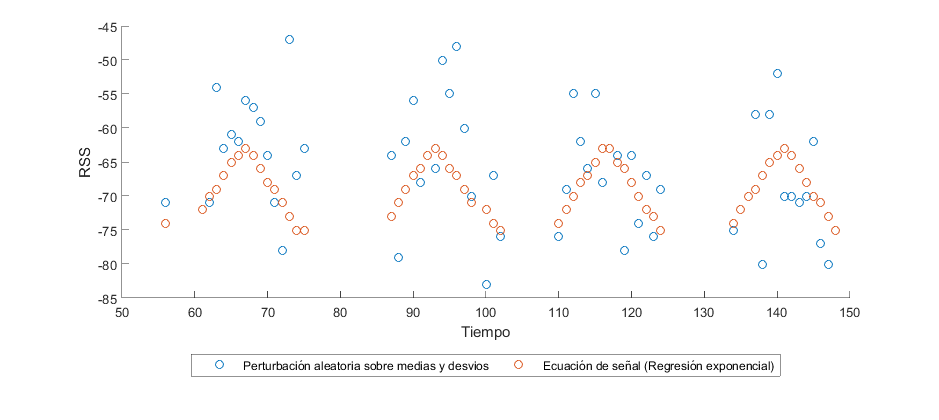
\includegraphics[width=0.8\textwidth]{images/simu-eq-vs-means.png}
	\captionsetup{width=0.7\textwidth}
	\caption{Ejemplo de simulación de un vehículo atravesando cuatro monitores, por ambos métodos. }
    \label{fig:eq-vs-means}
\end{figure}

Los datos generados por simulación son procesados por el algoritmo de Viterbi, extendido para soportar las observaciones $obs$ como un conjunto de eventos de \textit{deteccion} o \textit{nodeteccion}.

A fin de conocer el comportamiento real de las detecciones de un vehículo en movimiento se realizó un segundo experimento, el cual consistió en conducir a diferentes velocidades (20, 40, 60 y 80 Km/h) a través del rango de detección de un monitor. Tomando un segundo como unidad temporal, se consideró hacer un promedio de señales en los casos que el número de paquetes por unidad de tiempo sea $\frac{cant\_paq}{s}>1$.

Al no contar con referencia alguna sobre la distancia del vehículo respecto al detector, se hará la siguiente observación: se considera la marca temporal de la detección de mayor intensidad ($t_{maxdB}$) como momento de mayor proximidad al monitor (distancia $d_{maxdB}=0$).
A partir de la diferencia temporal $\delta_t$ de cada muestra respecto a $t_{maxdB}$, se calcula la distancia relativa $D(\delta_t)$ (dada la velocidad $v$) respecto a la ubicación $d_{maxdB}$ (Ecuación \ref{eq:distancia-velocidad}).
\begin{align}\label{eq:distancia-velocidad}
    D = \delta_t * v \frac{1000}{3600} 
\end{align}
En la Figura \ref{fig:speedtest} (Izquierda) se superponen las mediciones de las tres pruebas, conservando la distancia temporal relativa a $t_{maxdB}$,en cada caso. Aquí podemos observar que la señal respecto de la distancia se aproxima a una función de densidad gaussiana, incluso a velocidades de 80 Km/h.

\begin{figure}[!htp]
	\centering
	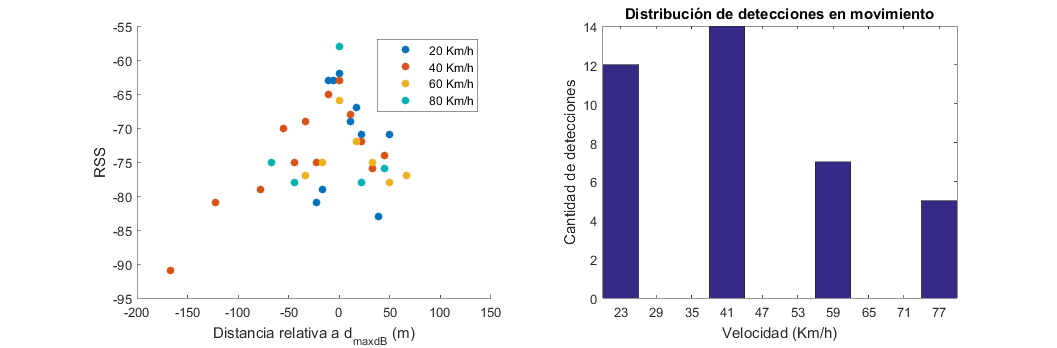
\includegraphics[width=\textwidth]{images/speedtest.png}
	\caption{Detecciones de las pruebas de velocidad}
    \label{fig:speedtest}
\end{figure}

En la distribución de detecciones según la velocidad (Figura \ref{fig:speedtest} - Derecha) puede observarse la baja densidad de detecciones al aumentar la velocidad. Esto se debe principalmente a que el vehículo permanece menos tiempo en la zona de detección del monitor. 

%%%%%%%%%% MODULO VITERBI

\section{Módulo Viterbi}\label{sec:viterbi}

Este módulo incluye algoritmos de estimación y manejadores para visualización de resultados. Los submódulos \textit{org.tte.logic} y \textit{jahmm.extensions} son dedicados a la estimación de tiempo de viaje aplicando el algoritmo de Viterbi y los métodos propuestos. La estimación de funciones de densidad (Sección \ref{sec:estimacionwireless}) se realiza desde la biblioteca de \textit{machine learning} Weka, en el paquete \textit{org.tte.kernelestimator}. El acceso a datos es realizado a través de una capa de abstracción implementada con Hibernate en \textit{org.tte.db}. En cuanto a las interfaces externas, el módulo de visualización es implementado en el paquete \textit{org.tte.app.beans} utilizando el framework Primefaces, basado en JavaServerFaces y, finalmente, se incluye una API Rest para obtener el estado actual de la red, desarrollada con el framework Spring.

\begin{figure}[!htp]
	\centering
	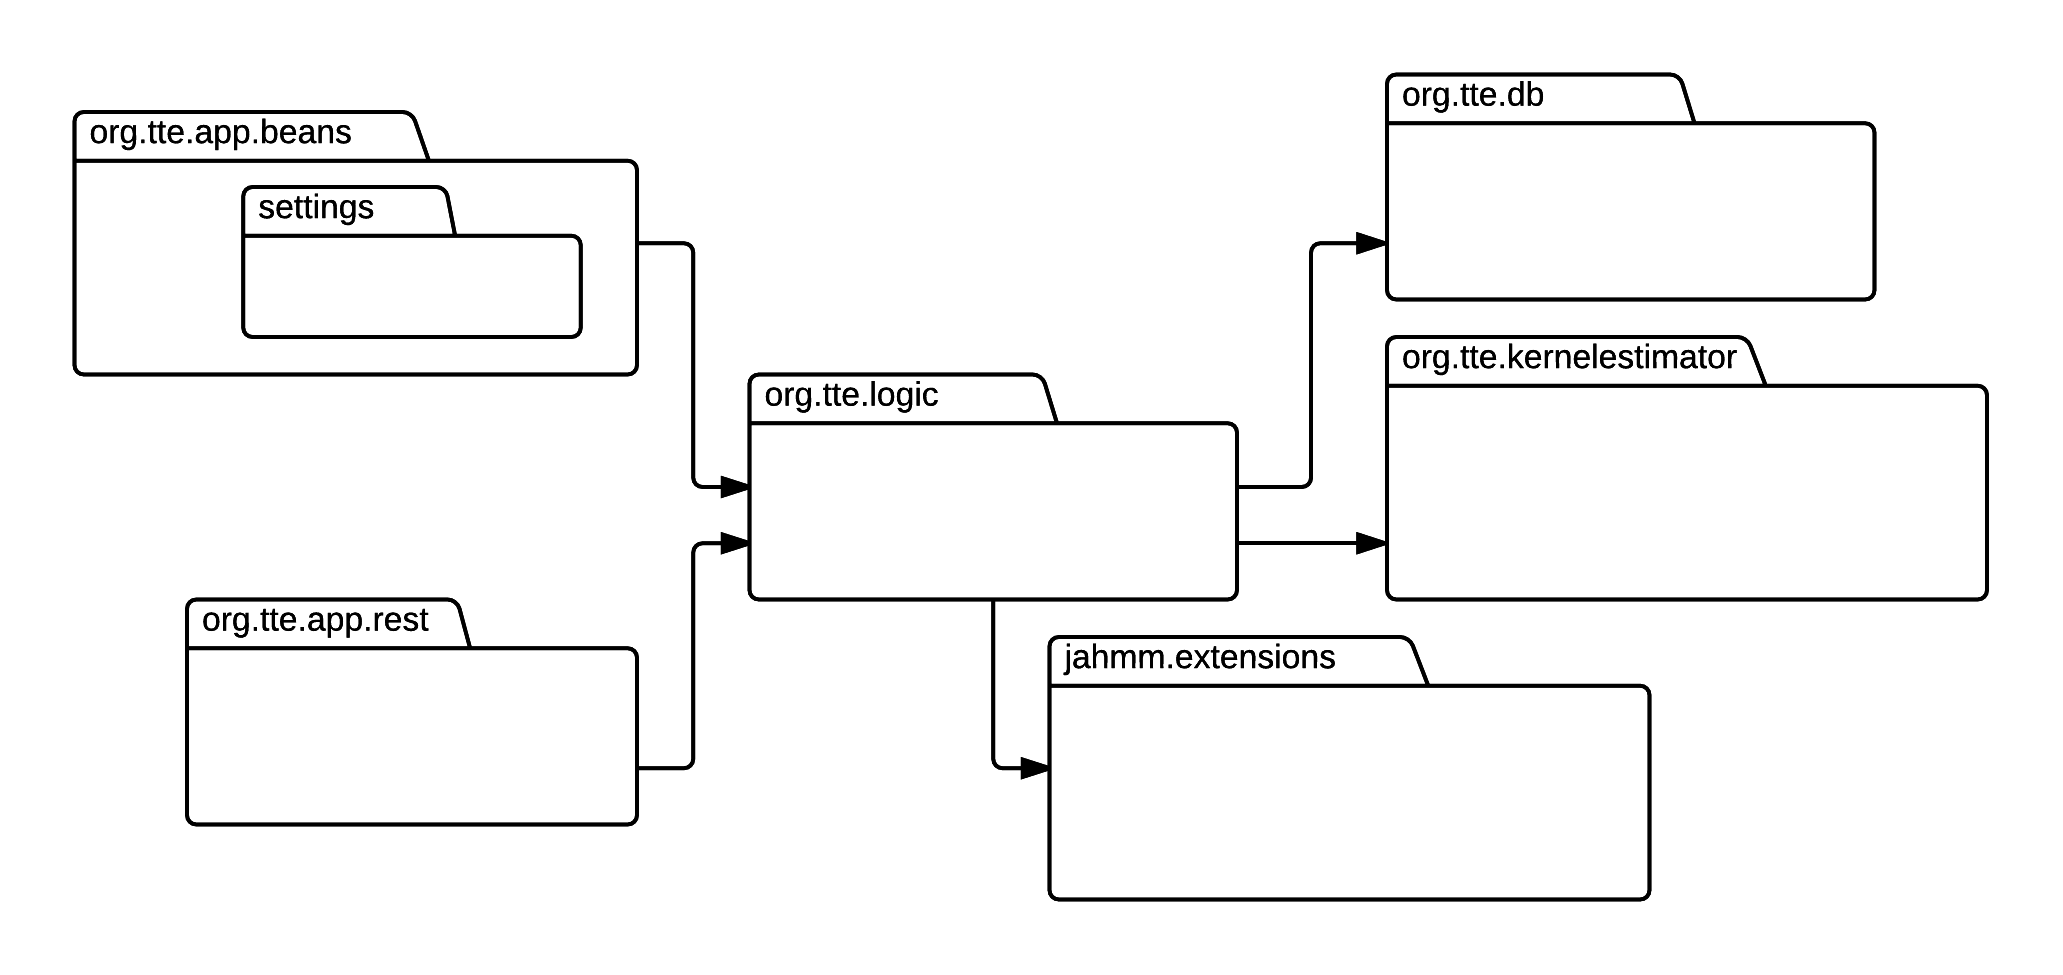
\includegraphics[width=0.9\textwidth]{images/modulos-viterbi.png}
	\caption{Vista de paquetes del módulo de estimación ``Viterbi''}
    \label{fig:cyc-estimacion}
\end{figure}

 La plataforma requiere un paso inicial de configuración: se debe cargar el mapa de la red (a partir del cual se generan los segmentos de $\mathcal{G'}$) y, además, se deben cargar las simulaciones (observaciones SUMO) generadas previamente. A continuación se presentan los detalles de implementación del módulo \textit{Viterbi}.

\subsection{Modelado de la red}

 Para segmentar la red en espacios mas cortos, es necesario partir de la red original. Esta puede ser importada a través de la ventana de ajustes de la aplicación. Se provee soporte de las especificaciones de mapas del proveedor OpenStreetMap (.osm). La red es almacenada en la base de datos bajo una estructura única de nodos (\textit{Node}) y arcos ({Edge}) \(\mathcal{G=<V,E>}\) (Figura \ref{fig:bbdd-viterbi}). Es necesario almacenar la estructura de $\mathcal{G}$ por la relación que conservan los datos de simulación con la estructura de la red. Estos datos se utilizan para dar estimaciones sobre los arcos originales (cuadras de la calle) y son visibles en los módulos de visualización para referencia. Adicionalmente, se almacena la ubicación, ganancia e identificador de cada monitor BT (\textit{AccessPoint} en el esquema de base de datos) desplegado en la red.
 
 \begin{figure}[!htp]
	\centering
	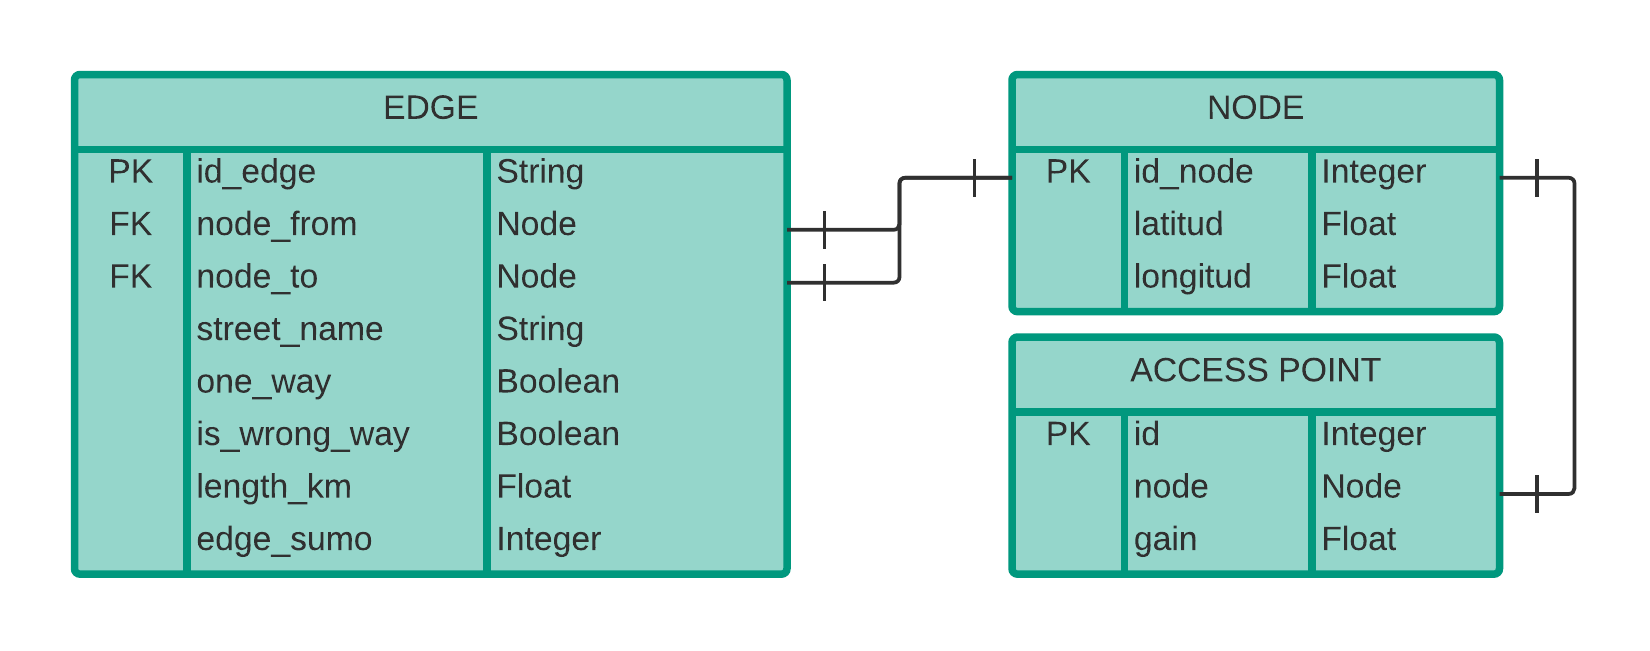
\includegraphics[width=0.7\textwidth]{images/bbdd-viterbi.png}
	\captionsetup{width=0.7\textwidth}
	\caption{Diagrama de Base de Datos correspondiente a la estructura de la red. Estas estructuras permanecen en el servidor PostgreSQL y dan soporte a los segmentos más cortos.}
    \label{fig:bbdd-viterbi}
\end{figure}

\subsection{Almacenamiento de datos}

 Todos los módulos que operan con la base de datos tienen como vía de acceso al componente \textit{DAOFacade} del paquete \textit{org.tte.db}. Este DAO (\textit{Data Access Object} u Objeto de Acceso a Datos) provee servicios para el alta y baja de: nodos, arcos y monitores BT. 
 
 \begin{figure}[!htp]
	\centering
	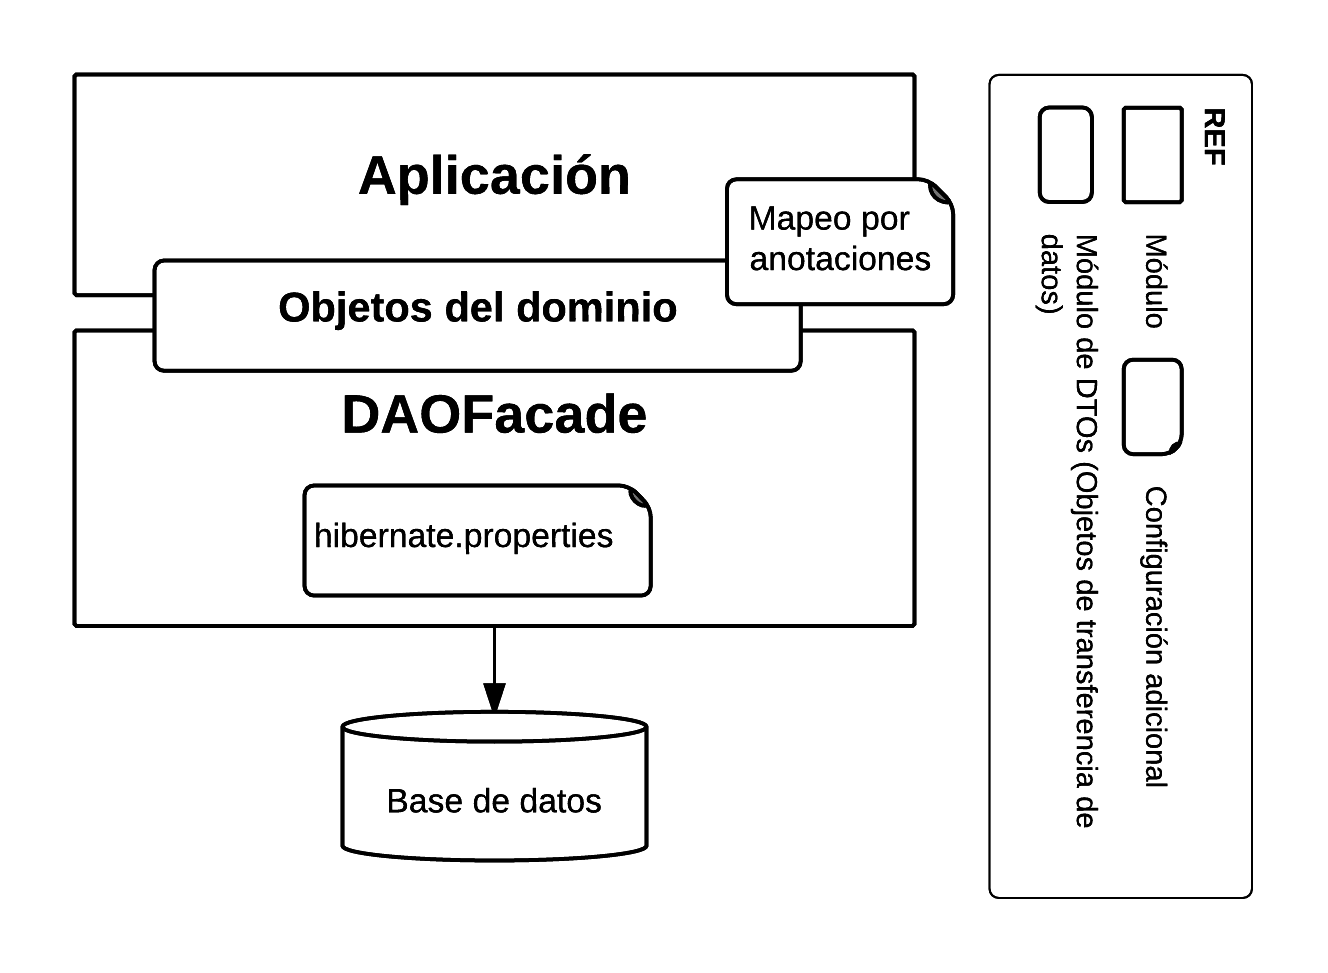
\includegraphics[scale=0.9]{images/hibernate.png}
	\captionsetup{width=0.7\textwidth}
	\caption{Vista de módulos para acceso a datos a través de Hibernate}
    \label{fig:hibernate}
\end{figure}
 
 El acceso a datos se implementó siguiendo el esquema basado en anotaciones del framework de persistencia open-source ``Hibernate''. Esta herramienta facilita el desarrollo de aplicaciones permitiendo hacer un mapeo de los objetos del dominio con las entidades de la base de datos. La configuración por anotaciones consiste en agregar ``decoraciones'' a los elementos de una clase. El código en \ref{alg:ej-hibernate} ilustra el mapeo de la tabla NODE con la correspondiente clase \textit{Node}. Se realiza agregando como encabezado de la clase la anotación \textit{@Entity} y a los atributos el encabezado \textit{@Column} e \textit{@Id} para la clave primaria de la relación.

\begin{lstlisting}[language=Java, caption=Mapeo objeto-relacional de la entidad Node en Hibernate, label=alg:ej-hibernate]
@Entity
public class Node {
    @Id
    private int id_node;
    @Column
    private  float latitud;
    ...
}
\end{lstlisting}

De forma similar se mapean las relaciones entre tablas, aquí se utilizaron relaciones 1-N para asociar los nodos de un arco (\text{Edge}) con la correspondiente tabla \textit{Node}. Para realizar el mapeo se agregan las anotaciones \textit{@ManyToOne}, \textit{Fetch} y \textit{@JoinColumn}. \textit{ManyToOne} indica que es un atributo relacionado, en lenguaje de definición de datos (DDL) se traduce a un campo con clave extranjera. \textit{Fetch} indica la estrategia de recuperación (se pueden recuperar sólo los datos de la entidad principal y no los relacionados). Al precisar tanto los arcos como los nodos, se utilizó el fetch vía JOIN que recupera los datos relacionados automáticamente. Finalmente, \textit{JoinColumn} permite definir el nombre de la comlumna en la BBDD, esto es en el caso de no coincidir con la nomenclatura de las variables. El extracto \ref{alg:ej-hibernate-edge} ejemplifica el mapeo del nodo \textit{NodeFrom} de un \textit{Edge}.

\begin{lstlisting}[language=Java, caption=Mapeo objeto-relacional de la entidad Edge en Hibernate, label=alg:ej-hibernate-edge]
@Entity
public class Edge {
	@Id
	private String id_edge;
	@ManyToOne
	@Fetch(FetchMode.JOIN)
	@JoinColumn(name="node_from")
	private Node nodeFrom;
	...
}
\end{lstlisting}


Para el despliegue de la aplicación se provee un archivo de configuración \textit{hibernate.properties} con datos de conexión y credenciales del servidor de base de datos PostgreSQL.  En la Figura \ref{fig:hibernate} se presenta el esquema de separación en ``\textit{capas}'' para el acceso a datos.

\subsection{Segmentación de la red}

Con el fin de obtener mayor granularidad en la estimación, la metodología desarrollada en la sección \ref{ssec:hmm-shortsegments} propone trabajar con la red \(\mathcal{G'=<V',E'>}\), compuesta por segmentos más cortos (SegmentoViterbi) que la longitud de una cuadra típica de una ciudad. Un \textit{SegmentoViterbi} contiene los cuatro vértices que lo define.

La longitud del segmento depende de la velocidad máxima de cada calle. Considerese, por ejemplo, una velocidad máxima $V_{MAX} = 80$ Km/h para una sección dada. Con un simple cambio de unidad a metros por segundo, ese dato nos dirá cuál es la distancia que se puede recorrer en un segundo ($L=22.2$ m). Se definió la unidad temporal entre observaciones en un (1) segundo. Se observa que un vehículo no podrá trasladarse entre segmentos no contiguos si se respetan los límites de velocidad. Esta es la granularidad que permite el modelo. En las pruebas realizadas, se utiliza una velocidad $V_{MAX}$ igual a la máxima velocidad entre todas las calles. Por otro lado, el ancho del segmento se calcula a partir de un $\alpha$ dado. Se pretende que el segmento cubra todos los carriles de la calle.

\begin{figure}[!htp]
	\centering
	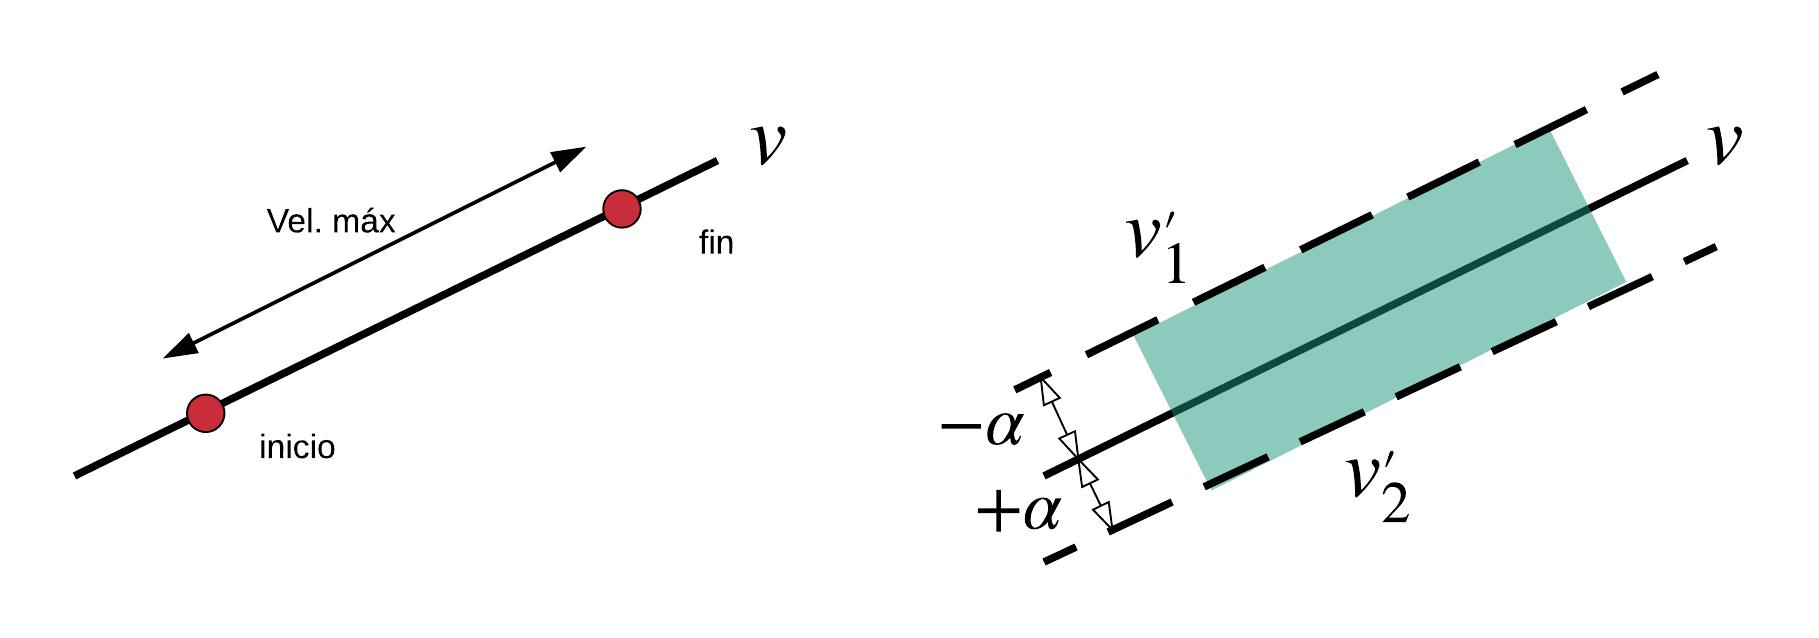
\includegraphics[width=0.8\textwidth]{images/segmentacion_mapa.png}
	\caption{Esquema del cálculo de los vértices de un segmento}
    \label{fig:segmentacion-mapa}
\end{figure}

La cantidad de segmentos que cubren a una calle se calcula como el techo de la división entre la longitud total de la calle y la longitud de un segmento. A partir de la cantidad de segmentos, se calcula por interpolación lineal el vector base $v = (p_{inicio},p_{fin})$ cuyas coordenadas se corresponden al inicio y fin de cada segmento sobre cada cuadra (Figura \ref{fig:segmentacion-mapa} - Izquierda) y, a partir de estos, se construye un \textit{SegmentoViterbi} calculando los cuatro vértices que definen al segmento (Figura \ref{fig:segmentacion-mapa} - Derecha).

El cálculo de los cuatro vértices se realiza con la biblioteca JavaGeom para procesamiento de líneas rectas en dos dimensiones. A partir de la línea $v$ se utiliza la función $parallel(\alpha)$ para calcular dos líneas $v_1'$ y $v_2'$ paralelas a $v$, que pasan por el punto $\alpha$. La separación entre líneas está dada por la distancia $\alpha$. Se fijó $\alpha = 0.000055$ (10 metros, tomado visualmente) para las evaluaciones realizadas.

% href{https://github.com/dlegland/javaGeom/blob/master/src/main/java/math/geom2d/line/Line2D.java}{Java2geom}

La Figura \ref{fig:capture-segments} ejemplifica la segmentación de una red de tránsito de un área urbana real. 

\begin{figure}[!htp]
	\centering
	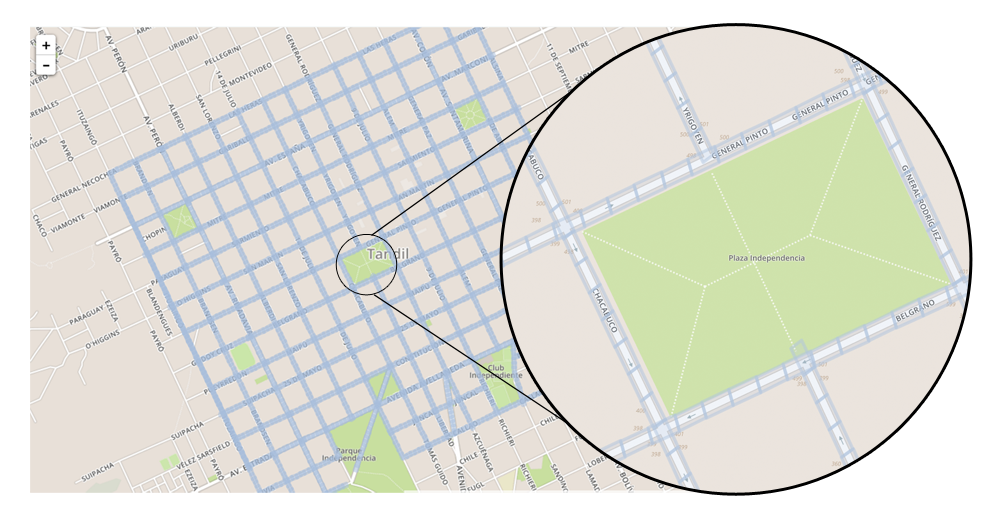
\includegraphics[width=0.7\textwidth]{images/capture-segments.png}
	\captionsetup{width=0.8\textwidth}
	\caption{Construcción de segmentos \textit{SegmentoViterbi} sobre la zona céntrica de la ciudad de Tandil. Dada una velocidad máxima $V_{MAX}=80$ Km/h, la longitud de un segmento es $L=22.22$ m. La cantidad total de divisiones asciende a 2.624 segmentos.}
    \label{fig:capture-segments}
\end{figure}

\subsection{Aplicación del algoritmo de Viterbi}

Para trabajar con el algoritmo de Viterbi, se seleccionó la biblioteca \textbf{Jahmm}\cite{Jahmm}, una implementación en el lenguaje de programación Java de los algoritmos que resuelven los problemas asociados a los HMM, descritos en el apartado \ref{ssec:problemashmm}. Es de código abierto, bajo la licencia BSD y fue diseñado para ser fácilmente utilizable y de propósito general. Además, cuenta con una interfaz a través de la línea de comandos para la ejecución de los algoritmos.

Provee implementaciones para varios algoritmos relacionados con los HMMs:

\begin{itemize}
\item Algoritmo de Viterbi 
\item Forward-Backward
\item Aprendizaje Baum-Welch
\item Aprendizaje K-Means
\item Kullback-Leibler (Estimación de distancia entre dos modelos)
\end{itemize}

Implementa, además, varias distribuciones de observación, entre algunas de ellas se encuentran: 

\begin{itemize}
\item Distribuciones a partir de un conjunto finito (ej. conjunto restringido de enteros)
\item Distribución Gaussiana
\item Distribución Gaussiana Mixta (múltiples distribuciones Gaussianas)
\item Distribución Gaussiana Multivariada.
\end{itemize}

Para comparar diferencias con los métodos propuestos, se utilizó la distribución Gaussiana multivariada (implementada por Jahmm) como distribución de observación de lecturas GPS. 

La herramienta provee una serie de generadores de observaciones pseudo-aleatorios para las distribuciones de observación que implementa. Sin embargo, estos no fueron utilizados ya que no cuentan con los parámetros de ajuste implementados por los métodos del módulo de simulación \textit{SumoUtils}.

Para poner en contexto las extensiones realizadas sobre la biblioteca, es necesario introducir la división en paquetes de la misma. Sólo se describen los paquetes que corresponden a la representación de los modelos, algoritmos y distribuciones de observación:

\begin{description}
\item [be.ac.ulg.montefiore.run.jahmm:] Es el paquete principal, contiene las definiciones de HMMs, observaciones y funciones de distribución de probabilidades de observación. También contiene las implementaciones de los algoritmos de Viterbi y Forward-Backward
\item [be.ac.ulg.montefiore.run.jahmm.learn:] Contiene los algoritmos de aprendizaje (algoritmos que ajustan los modelos a las observaciones)
\item [be.ac.ulg.montefiore.run.distributions:] Contiene implementaciones de las distribuciones de observación disponibles.
\end{description}

 La flexibilidad de la herramienta se centra en el uso de tipos genéricos para la definición del HMM (Figura \ref{fig:jahmm-modulos}). Es necesario instanciar el modelo con los parámetros: $\pi$, $a$ y $opdfs$ (Sección \ref{ssec:algoritmo-viterbi}). Para la representación de observaciones y OPDFs, Jahmm cuenta con clases abstractas e interfaces, respectivamente. 

\begin{figure}[!htp]
	\centering
	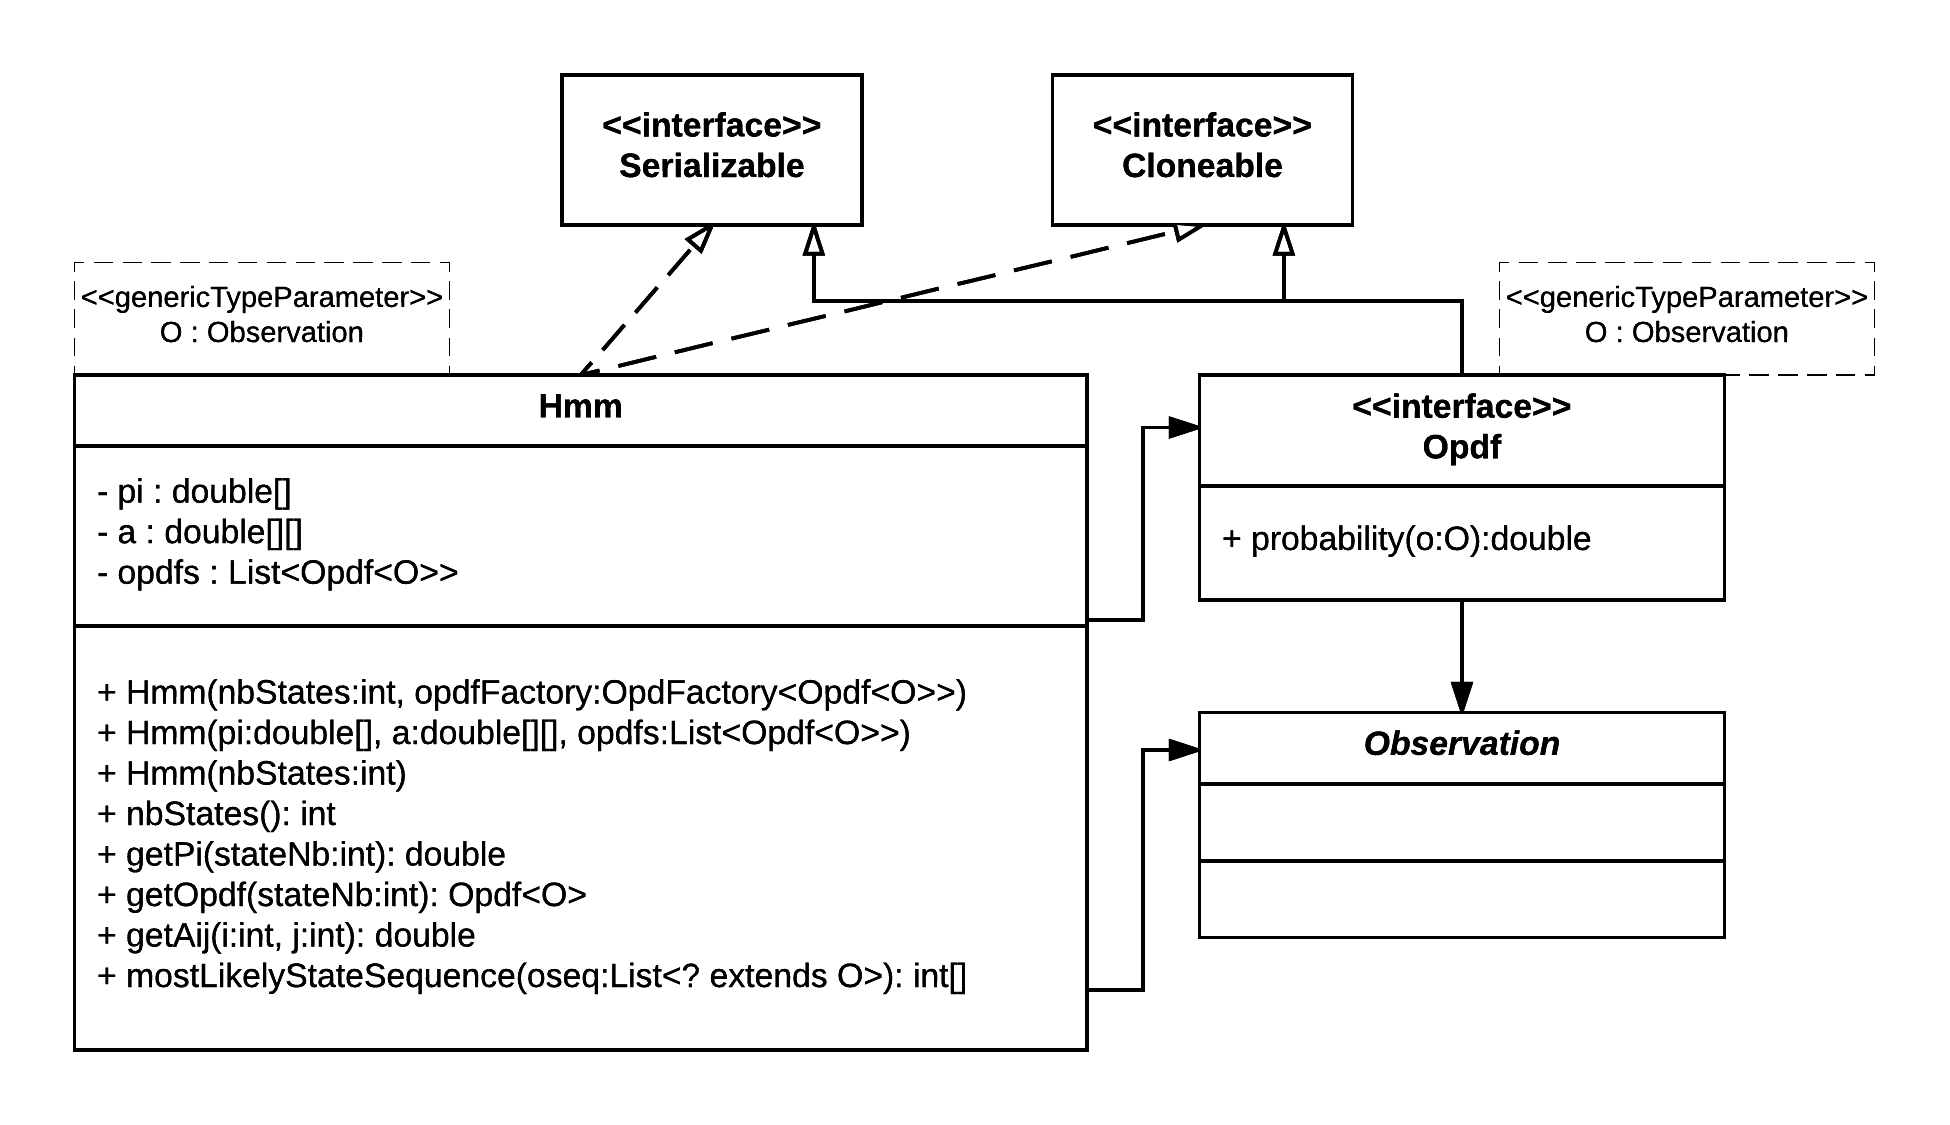
\includegraphics[width=0.9\textwidth]{images/jahmm-modulos.png}
	\captionsetup{width=0.8\textwidth}
	\caption{Clases e interfaces para la representación del Hmm en Jahmm}
    \label{fig:jahmm-modulos}
\end{figure}

El componente principal es la clase \textit{Hmm}. Provee las interfaces necesarias para definir el modelo y ejecutar los algoritmos. El constructor utilizado es el que toma todos los parámetros de un Hmm como argumento: $\pi$ (valores de probabilidad inicial), $a$ (matriz de transición de estados) y $opdfs$ (distribuciones de observación), o bien, $(pobs|s)$. Cabe aclarar que la cantidad de estados se corresponde con las dimensiones de los parámetros, es decir, está implícita. Si se define la cantidad de estados, los parámetros deberán conservar la misma dimensión. De este modo, los estados de un modelo llevan como número de identificación al índice asociado a los parámetros. Por ejemplo, el estado 0 tendrá probabilidad inicial $\pi_0$, probabilidades de transición $a_{0,j}$ y probabilidades de observacion $opdfs_{0}$. La estimación de los estados más probables será, entonces, un arreglo de enteros que sigue la identificación interna (\textit{mostLikelyStateSequence(List<? extends O>):int[]}).

\begin{figure}[!htp]
	\centering
	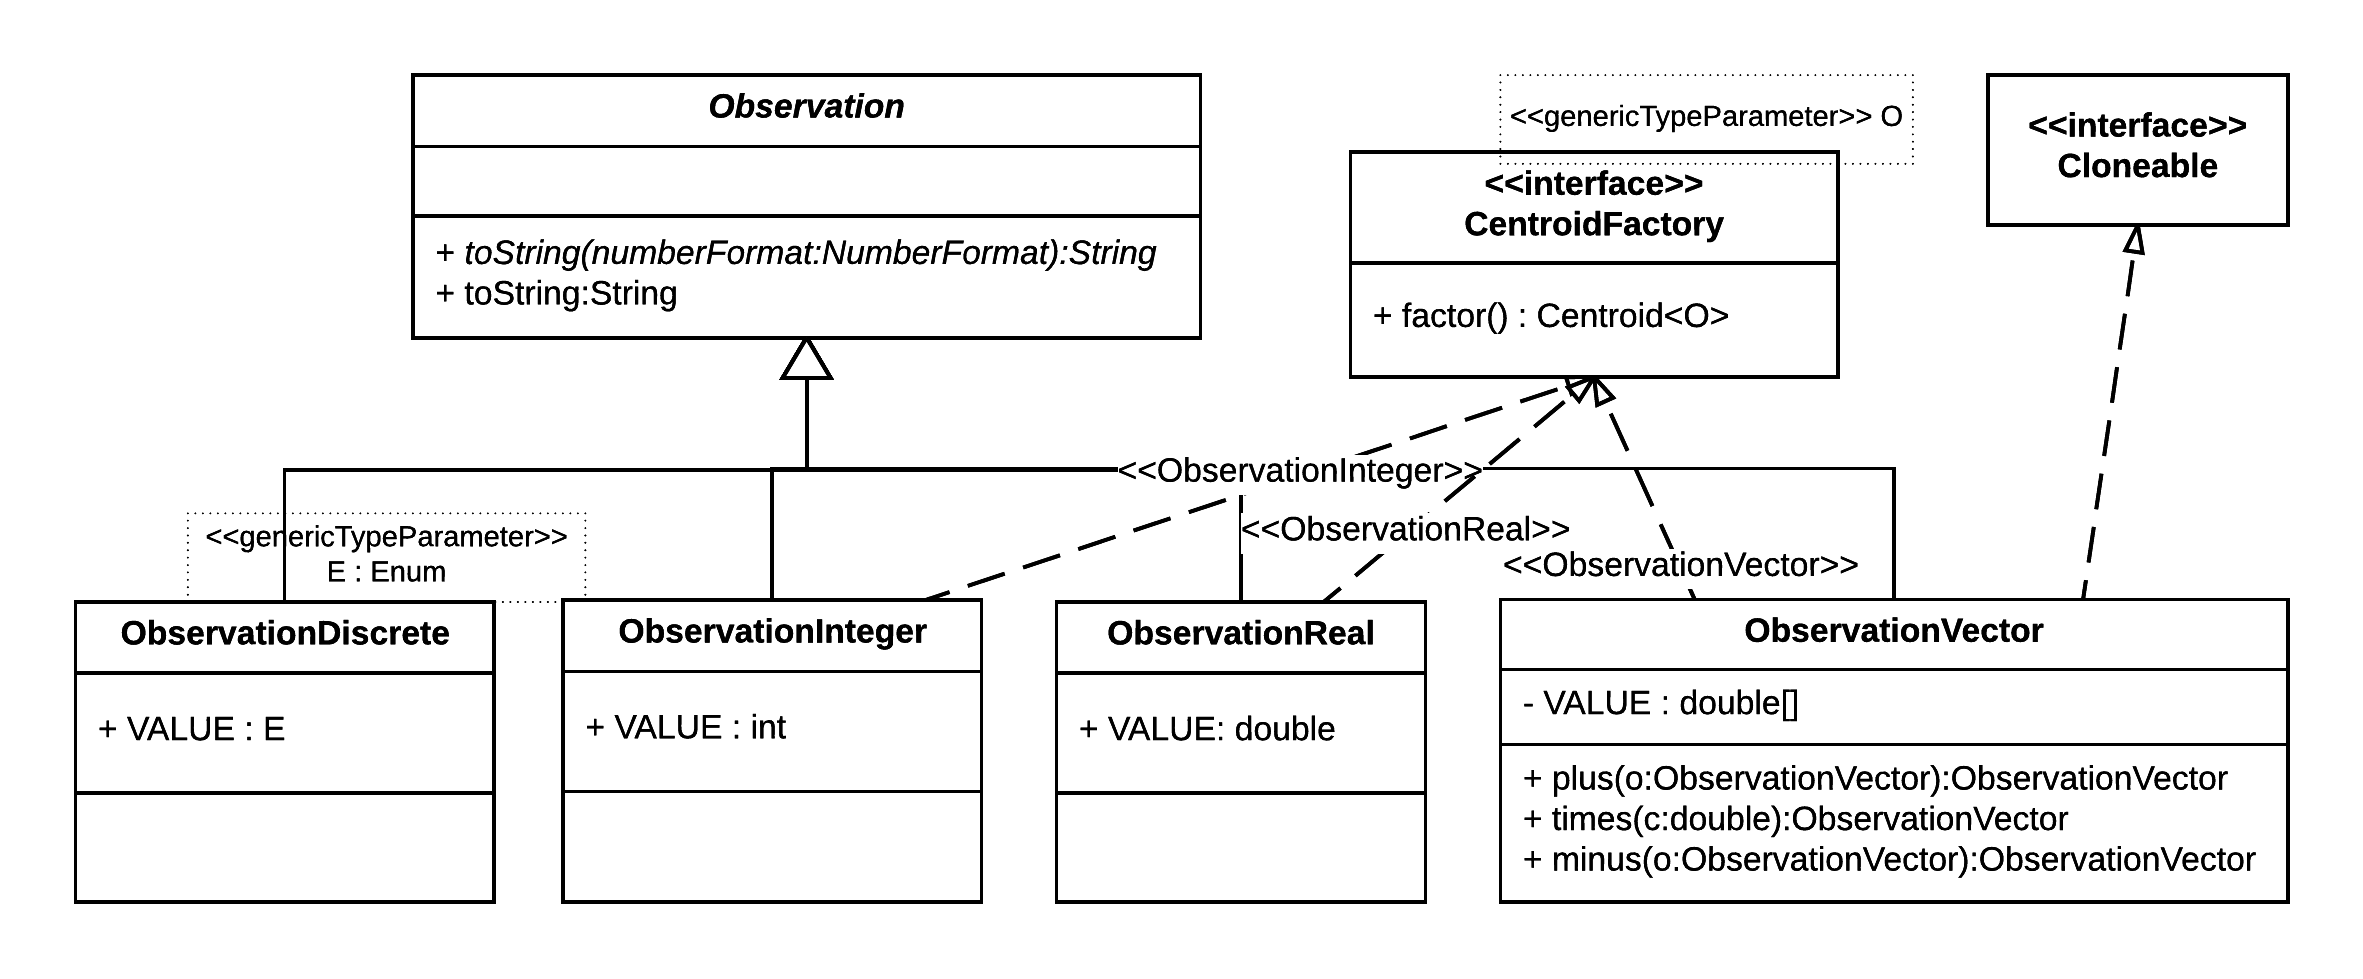
\includegraphics[width=0.9\textwidth]{images/jahmm-obs.png}
	\captionsetup{width=0.7\textwidth}
	\caption{Diagrama de clases que extienden \textit{Observation}}
    \label{fig:jahmm-obs}
\end{figure}

Entre los distintos tipos de observación provistos por la herramienta (Figura \ref{fig:jahmm-obs}), se encuentran las Observaciones discretas (por ejemplo, en el caso del casino deshonesto, los valores de los dados se pueden representar con un enumerado de enteros del 1 al 6). También se incluyen observaciones enteras (sin restricciones) y observaciones en los reales (por ejemplo, para mediciones de velocidad, o temperaturas). Finalmente, se encuentran las observaciones \textit{ObservationVector} como un vector de variables de punto flotante. \textit{ObservationInteger}, \textit{ObservationReal} y \textit{ObservationVector} implementan la interfaz \textit{CentroidFactory}, estos son componentes adicionales que permiten generar observaciones aleatorias en los valores comprendidos por cada tipo de observación.

En este trabajo, se parametriza la clase \textit{Hmm} con los tipos de observación \textit{ObservationVector} (para observaciones GPS), y \textit{ObservationEventVector} (para observaciones Bluetooth).  \textit{ObservationVector}.

\subsubsection{Procesamiento de señales}
Las observaciones son construidas a partir de archivos de observaciones SUMO (los ya mencionados Smartphone detections y Bluetooth Detections) que representan diferentes simulaciones cargadas en la plataforma. La carga de un nuevo archivo se realiza a través del panel de ajustes (Figura \ref{fig:captura-settings-gps}).


\begin{figure}[!htp]
	\centering
	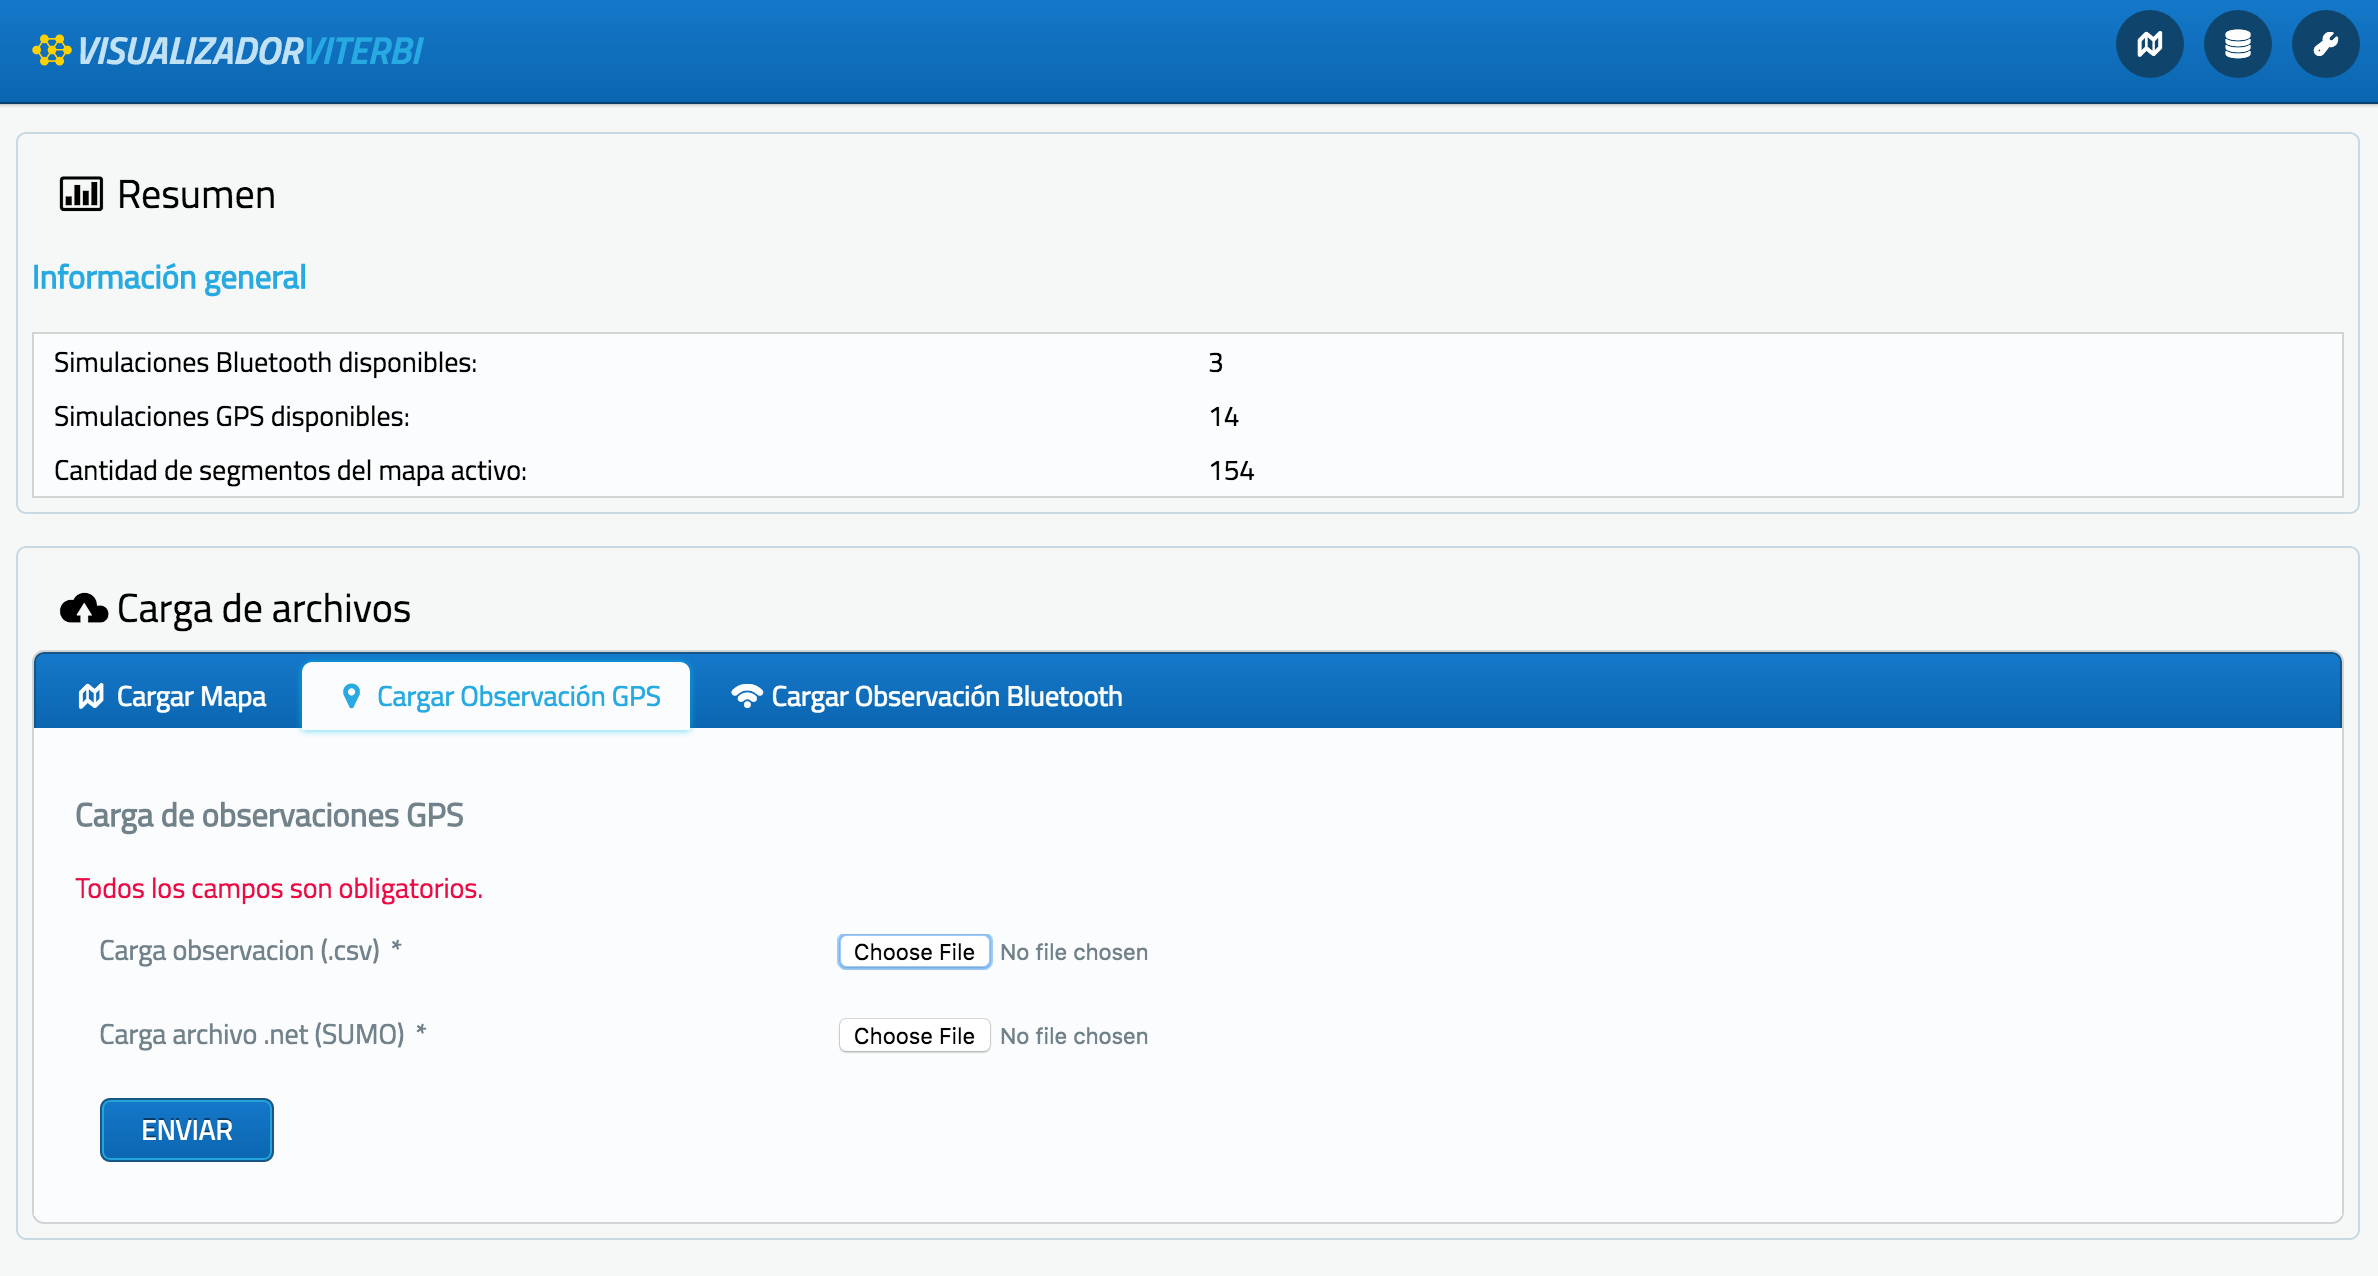
\includegraphics[width=0.8\textwidth]{images/captura-settings-gps.png}
	\captionsetup{width=0.8\textwidth}
	\caption{Captura de pantalla del panel de ajustes de la plataforma.}
    \label{fig:captura-settings-gps}
\end{figure}

El módulo SumoUtils aplica diferentes procesos a las observaciones cargadas. En el caso de observaciones GPS, se corrige la traslación original introducida por \textit{SUMO}. En el caso de observaciones Bluetooth, la simulación de la señal se realiza según el método que se quiera aplicar (ecuación por regresión exponencial ó  aleatorización basada en medias y desvíos).


La estructura de observaciones \textit{ObservationVector} (del paquete \textit{be.ac....run.jahmm}), es válida para el procesamiento de observaciones GPS. Esto es por tratarse de coordenadas en punto flotante (\textit{lat,lng}). En el caso de una observación Bluetooth, se agrega un nuevo tipo de observación: \textit{ObservationEventVector}. 

\subsection{Probabilidades de emisión GPS}

Los métodos propuestos para la estimación de trayectorias a partir de observaciones GPS son desarrollados como implementaciones de la interfaz \textit{Opdf<O>}, parametrizada con \textit{ObservationVector}. Esta interfaz define el método \textit{probability(O)}, utilizado por la implementación del algoritmo de Viterbi (método \textit{mostLikelyStateSequence(List<O>)}, de la clase \textit{Hmm}). Concretamente, 
\textit{probability(O)} debe resolver el cálculo de la probabilidad de realizar la observación \textit{O} dado que el estado es s, o bien: \textit{p(O|s)}. Si bien las OPDF permanecen asociadas a cada estado (segmento), no es posible recuperar información sobre el segmento a menos que explícitamente se agreguen estos datos a la OPDF. 

\begin{figure}[!htp]
	\centering
	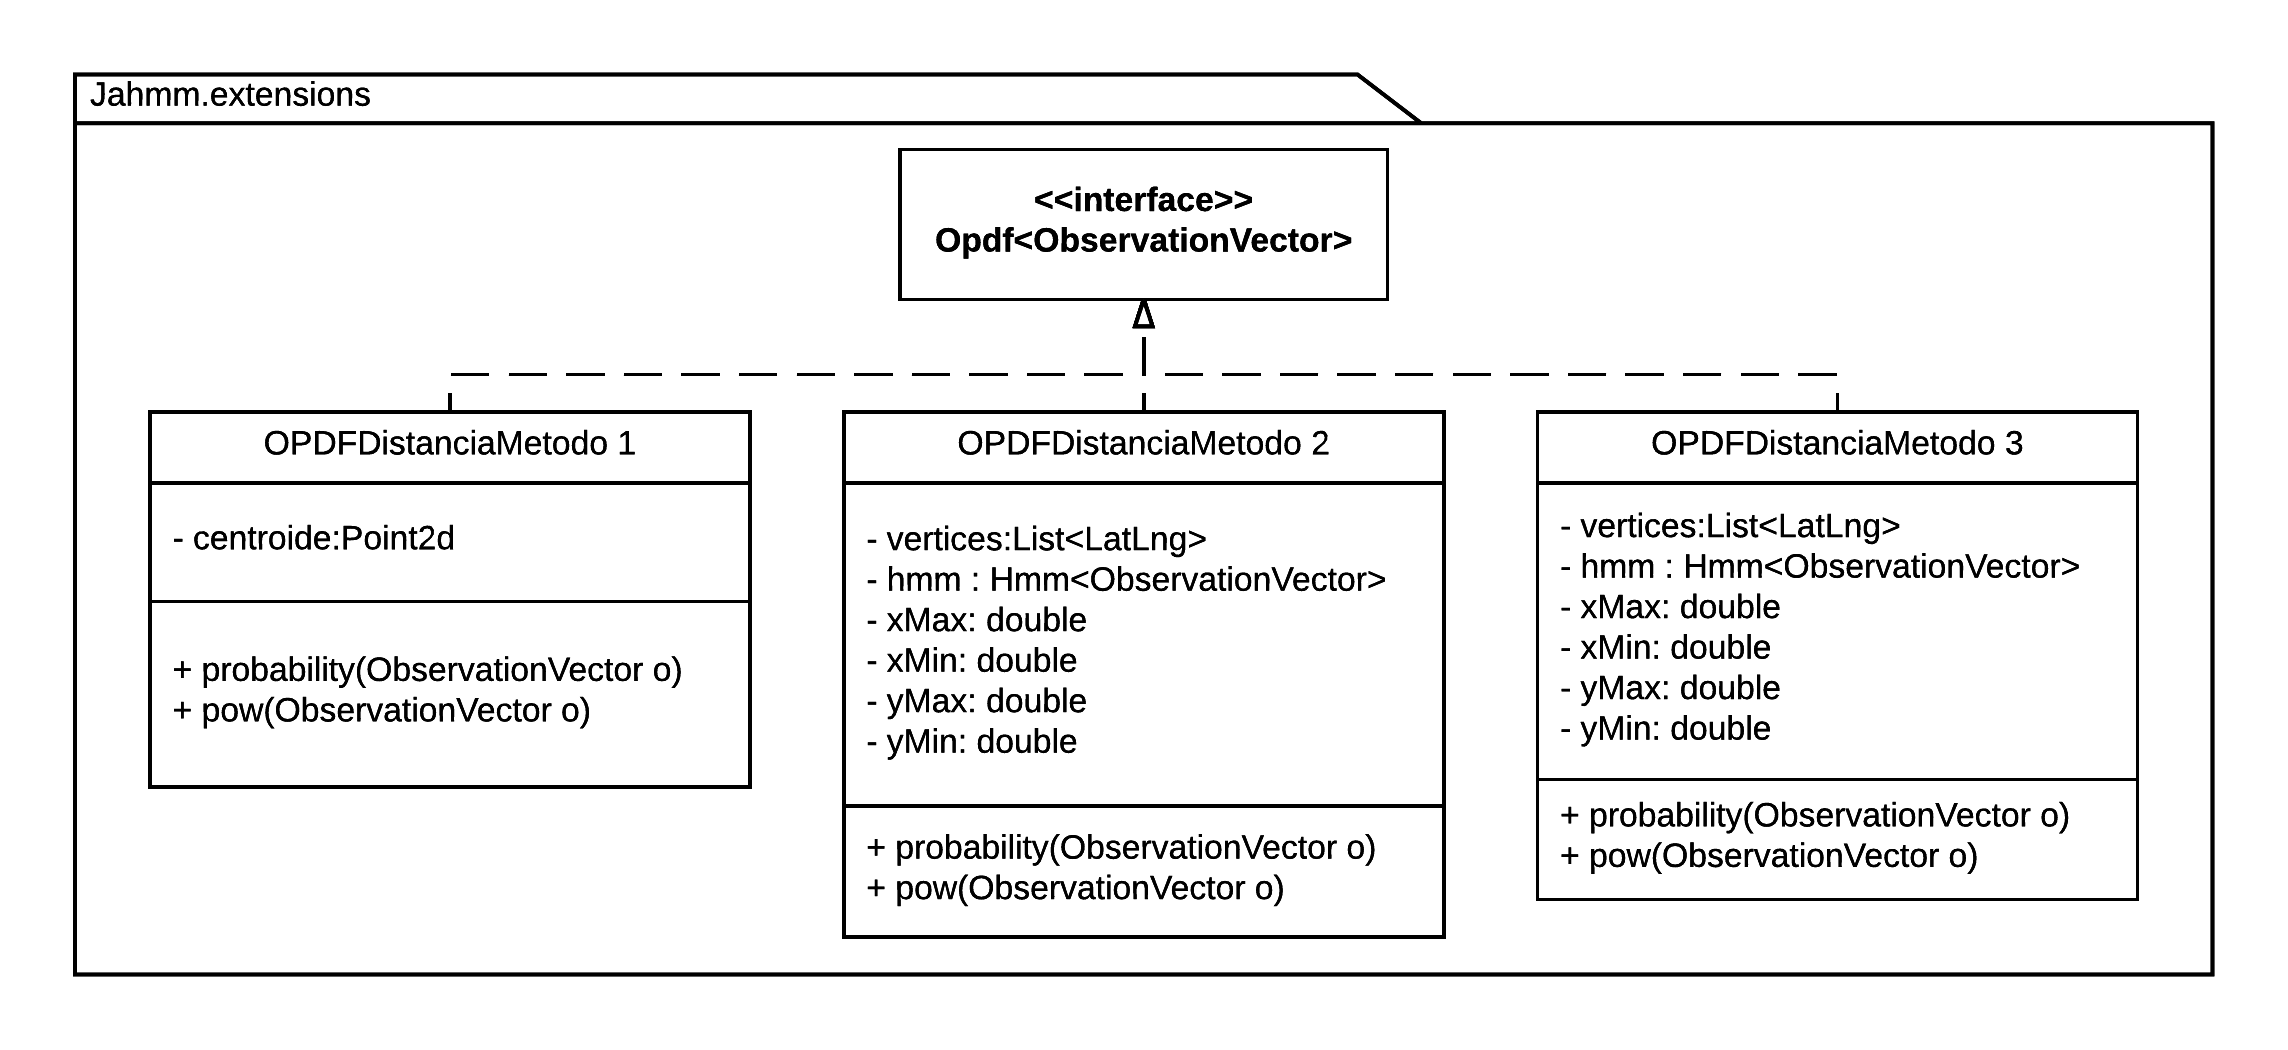
\includegraphics[width=0.8\textwidth]{images/jahmm-gps.png}
	\caption{Implementación de los métodos de estimación GPS como extensiones de Jahmm}
    \label{fig:jahmm-gps}
\end{figure}

El \textit{Método 1} (Apartado \ref{sssec:metodo1}), basado en la distancia entre la observación y el centro del segmento, precisa contar con la coordenada asociada al segmento. Se agrega entonces una propiedad en la OPDF para conservar la posición central del segmento. Posteriormente, se utilizará para resolver $p(obs|s)$. De forma similar, el método 2 (definido en \ref{sssec:metodo2}) requiere los vértices que definen a cada segmento para el cálculo de la probabilidad de observación sobre la superficie del segmento. Para obtener los límites de cada superficie se calculan los puntos máximos y mínimos (en \textit{x} e \textit{y}) entre los 4 vértices.

\subsection{Probabilidades de emisión Bluetooth}

Aquí, $p(obs|s)$ contesta a la pregunta: ``Si el dispositivo estuvo aquí, ¿cuál es la probabilidad de que hiciéramos la observación que acabamos de hacer?''

Para dar soporte al conjunto de detecciones (y no detecciones) de todos los monitores en un instante dado  (apartado \ref{sec:estimacionwireless}), se define el nuevo tipo \textit{ObservationEventVector} para observaciones Bluetooth. Por las características de la observación, es preciso contar con una estructura más completa, como lo refleja la Figura \ref{fig:jahmm-eventvector}.

\begin{figure}[!htp]
	\centering
	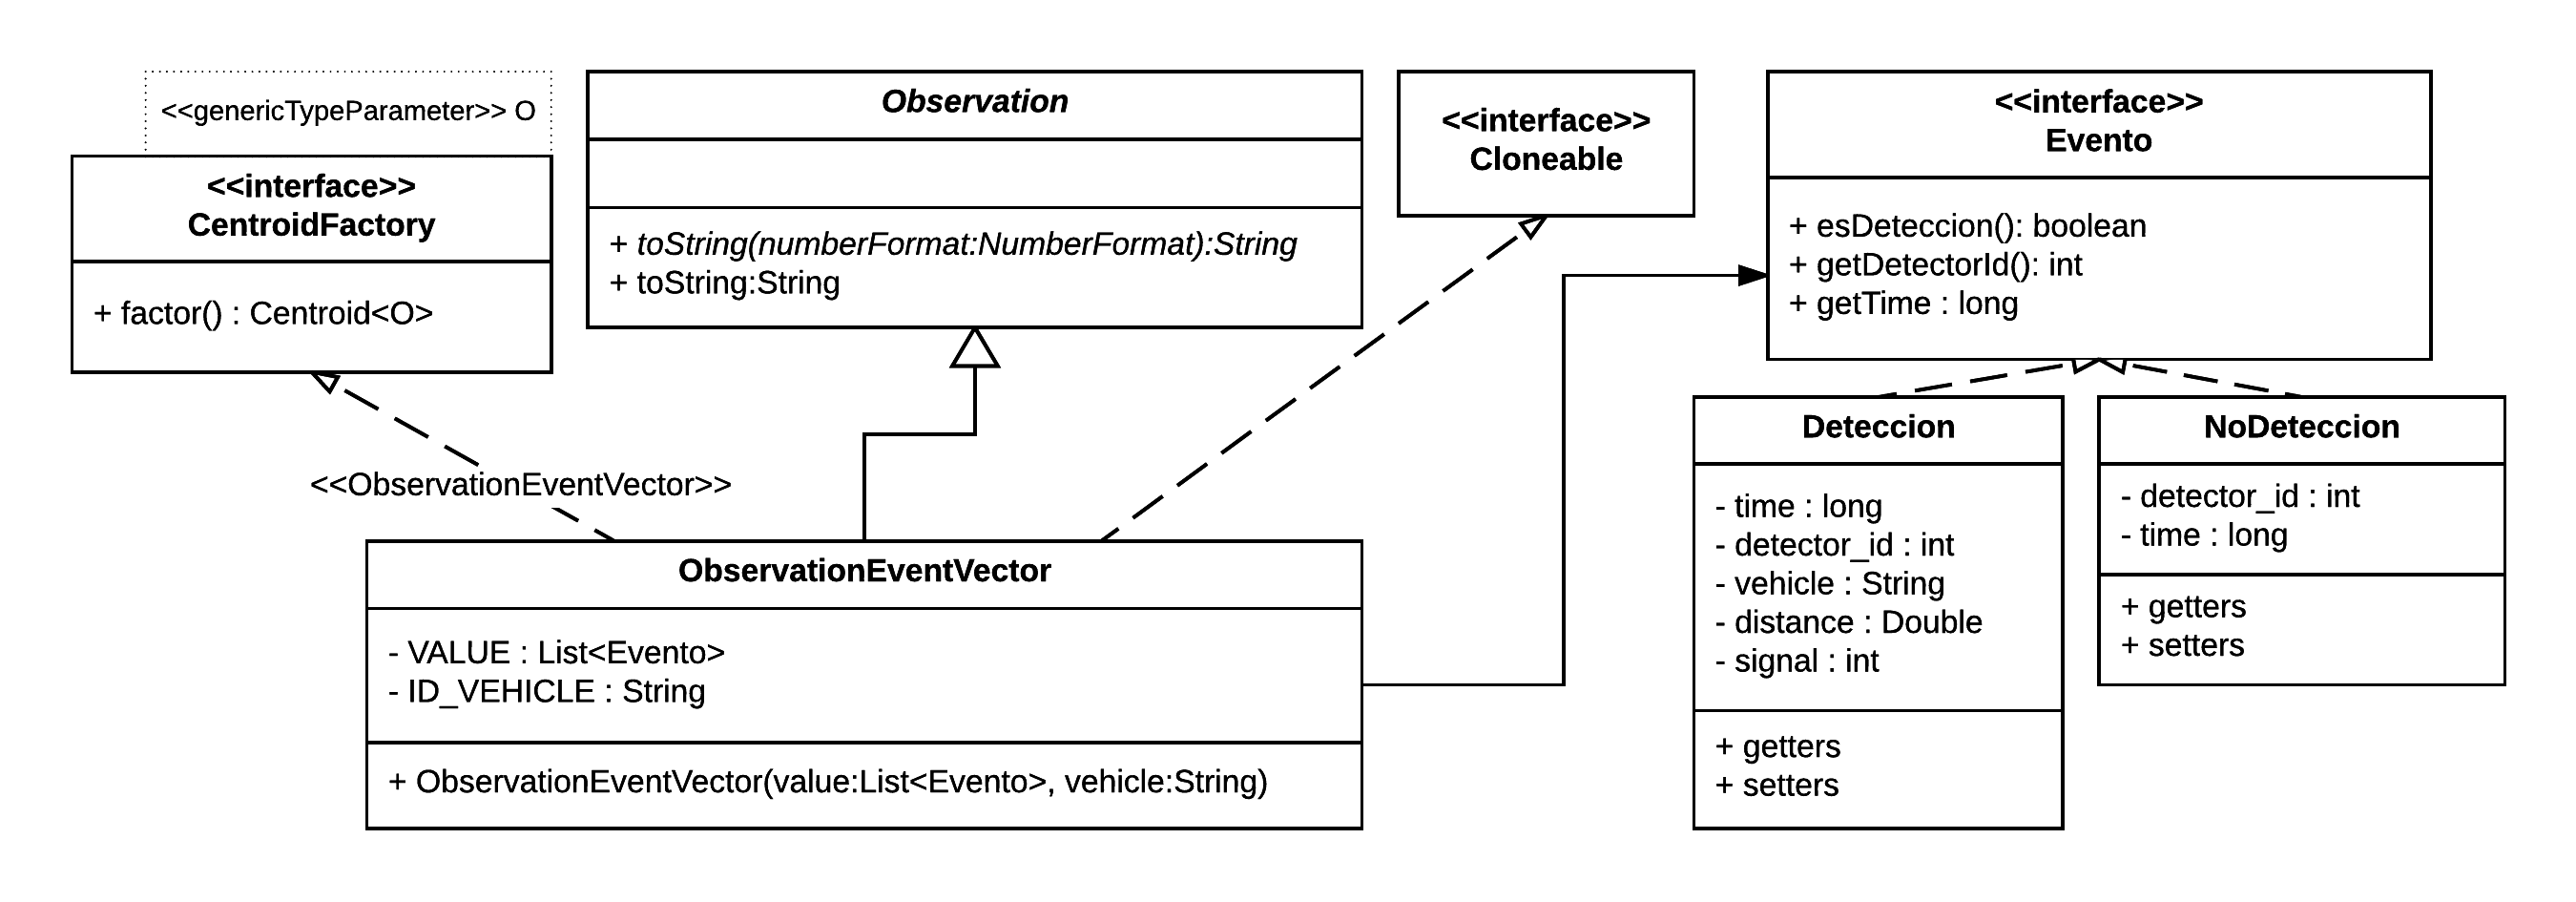
\includegraphics[width=0.9\textwidth]{images/jahmm-eventvector.png}
	\captionsetup{width=0.8\textwidth}
	\caption{Extensión de Jahmm \textit{ObservationEventVector} para observaciones Bluetooth}
    \label{fig:jahmm-eventvector}
\end{figure}

La estructura posee los detalles de cada observación (conjunto de detecciones), necesarios para la estimación y posterior análisis y resumen de resultados. La probabilidad de observación, en este caso, sigue la ecuación \ref{eq:observacion}, donde se realiza el producto de las probabilidades de \textit{detección}, para cada monitor.

Dada \textit{obs}, $p(e_m|s,tx)$ depende de si el evento $e_m$ es una \textit{detección} o una \textit{no-detección}. En el caso de una detección, se calcula como $p(dist|RSS)$. Aquí se utiliza la \textit{OPDF} asociada al estado $opdf_s$ para calcular la probabilidad (estimada) de haber observado la señal \textit{RSS} a distancia \textit{dist}. Los métodos propuestos se asemejan a las variaciones de los métodos GPS: en el primer caso, se evalúa la función \textit{opdf} a partir de la distancia del Monitor \textit{m} al centro del segmento \textit{s} (\textit{OPDFSignalDistance}). Como la distancia de cada monitor a los segmentos es invariante, este cálculo se realiza al construir el modelo, a partir de la función \textit{calculateAPDistances()}, para todos los segmentos y monitores.

\begin{figure}[!htp]
	\centering
	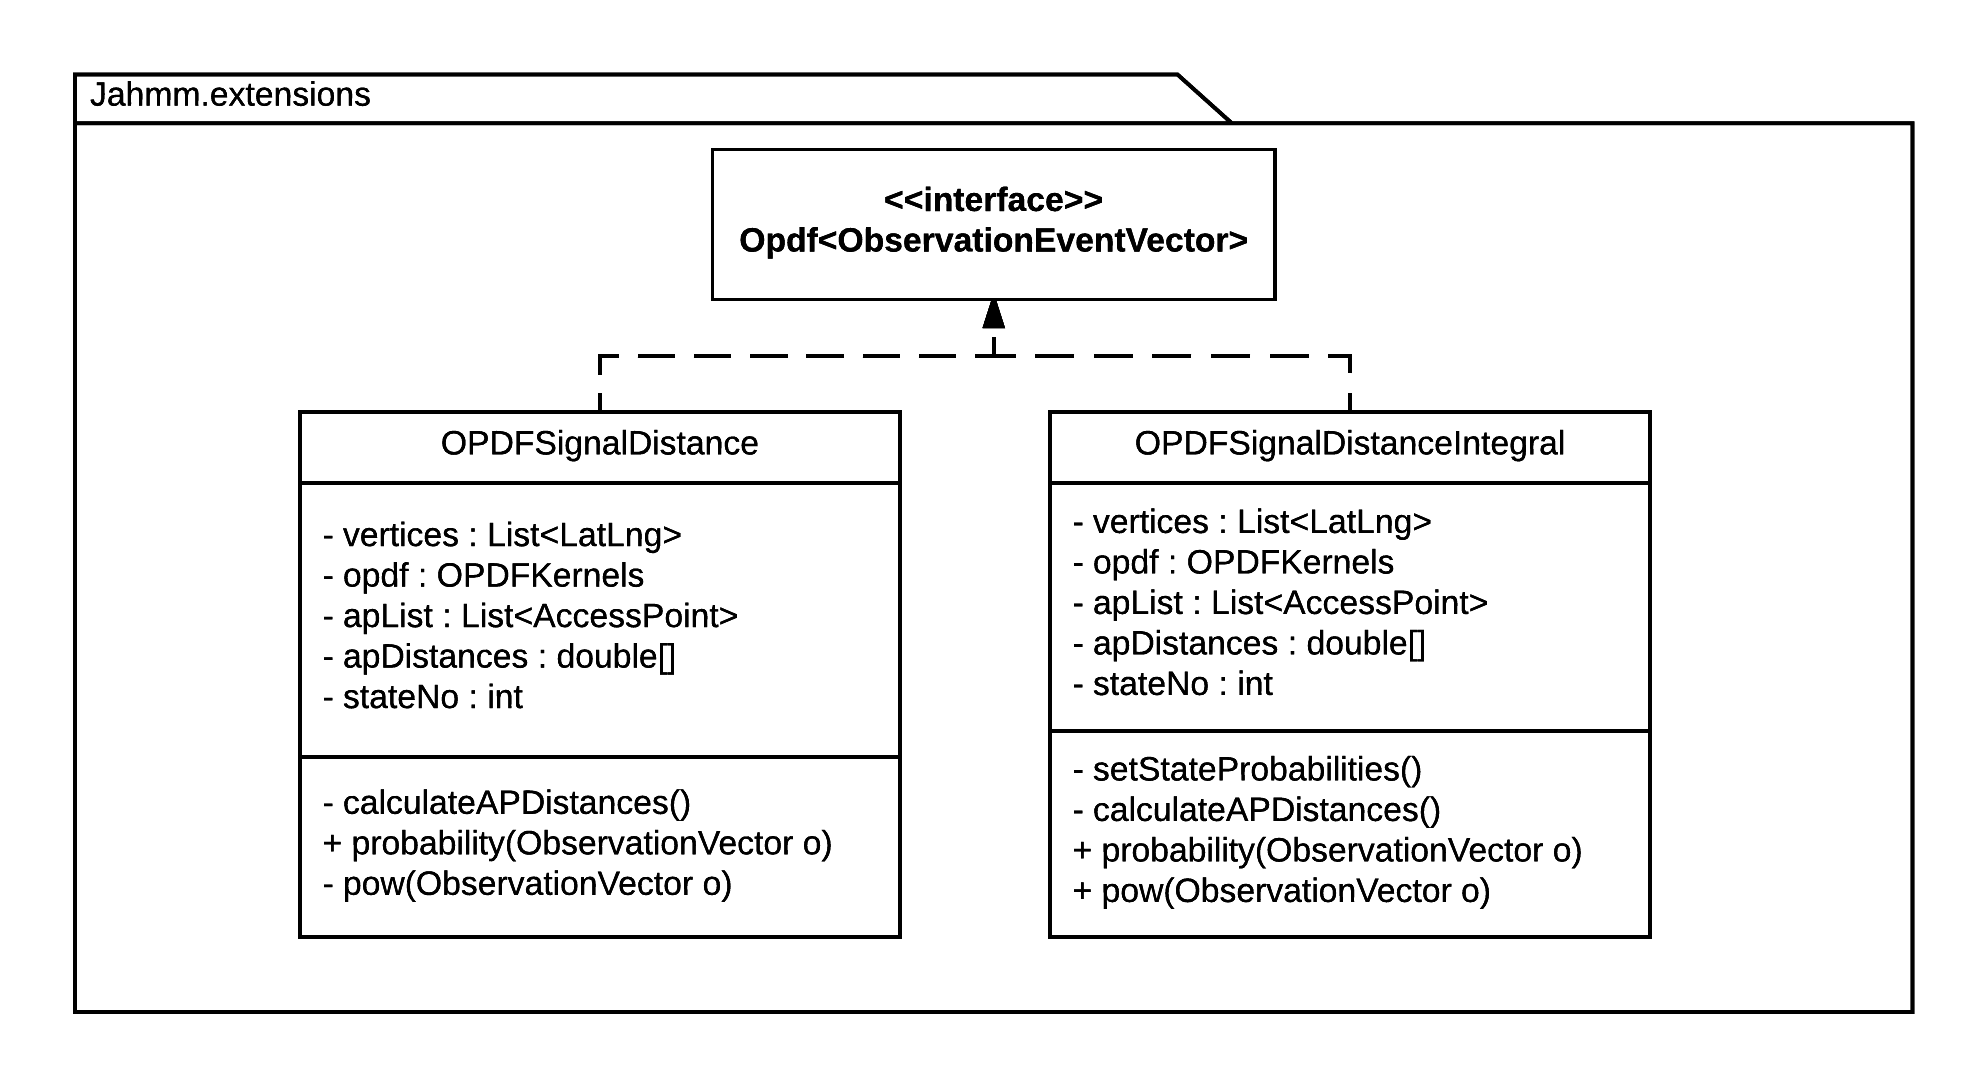
\includegraphics[width=0.9\textwidth]{images/jahmm-bluetooth.png}
	\captionsetup{width=0.8\textwidth}
	\caption{Extensión de Jahmm: Función de densidad de probabilidades \textit{Opdf<ObservationEventVector>} para observaciones Bluetooth}
    \label{fig:jahmm-bluetooth}
\end{figure}

En el caso de \textit{OPDFSignalDistanceIntegral}, la implementación del método realiza el cálculo de $p(deteccion_m|s,tx) = \int_s p(dist|RSS) dxdy$ llevando a cabo una suma de las probabilidades de todas las distancias de un monitor a un espacio de puntos discreto sobre la superficie del segmento. Para generar el espacio discreto se divide el segmento por el ancho y alto en $\delta$ unidades. Se recorre el espacio como $x_i = x_{inicio} + \delta * i$, para $x_i$ y, del mismo modo, se define $y_i$.


\subsection{Función de densidad de probabilidades de observación}\label{ssec:kernel}

Introducido en la sección \ref{sec:estimacionwireless}, $p(deteccion_m|s,tx)$ se obtiene aplicando un estimador de funciones de densidad sobre el conjunto de datos recolectados por experimentación, detallado en el apartado \ref{ssec:bt-simulation}. 

Las intensidades de señal se registran como valores enteros dentro de un rango de señal muy amplio. Las lecturas realizadas experimentalmente no son suficientes para caracterizar cada valor entero posible de RSS. En su lugar, se divide la intensidad de señal en rangos. Se consideró contar con al menos 200 lecturas en cada rango, por lo cual se definieron 5 rangos cumpliendo con los requerimientos:

\begin{itemize}
    \item Mayores a -60 dB
    \item Entre -60 dB y -65 dB
    \item Entre -65 dB y -70 dB
    \item Entre -70 dB y -75 dB
    \item Menores a -75 dB 
\end{itemize}

Sobre el conjunto de pares distancia-señal capturados se realiza una estimación no paramétrica de funciones de densidad de probabilidad, o ``método kernel''. 

Suponiendo que se cuenta con un conjunto de datos de una muestra con función de densidad de probabilidad desconocida, la estimación de densidad consiste en la construcción de una función de densidad estimada de los datos observados.

Un enfoque de estimación de densidad es el paramétrico. Asume que los datos fueron arrojados de una familia de distribuciones paramétricas conocida, como por ejemplo la distribución normal con media $\mu$ y varianza $\sigma^2$. La densidad subyacente a los datos ($f$) es entonces estimada buscando aproximaciones de ambas variables. En el enfoque no paramétrico, por el contrario, no se hacen suposiciones estrictas acerca de la distribución de los datos observados.

Entre los métodos más utilizados para la estimación de densidad no paramétrica, se encuentra el método por histograma y el método Kernel. El histograma es el más sencillo y, por esto, el más utilizado. La diferencia básica entre el histograma como técnica de representación de datos o como estimador de densidad es que en este último caso debe estar normalizado para integrar 1. 

La discontinuidad de los histogramas causa dificultades si se requieren derivadas de las estimaciones. Cuando las estimaciones son necesarias como componentes intermedios de otros métodos, se tiende a utilizar métodos mas sofisticados\cite{silverman1986density}. En este trabajo se propone utilizar la estimación tipo Núcleo \textit{(Kernel)}.

\subsection*{Definición}

Dada la muestra de $n$ observaciones reales $X_1,...,X_n$ se define la estimación tipo Kernel de función núcleo K como
\begin{align}
\hat{f}(x) = \frac{1}{nh_n} \sum_{i=1}^{n} K\left (\frac{x-X_i}{h} \right)
\end{align}

donde K(x) es una función, denominada función Kernel, función núcleo o función peso, que satisface ciertas condiciones de regularidad, generalmente es una función de densidad simétrica como por ejemplo la distribución normal, y $\{h_n\}$ es una secuencia de constantes positivas conocidas como ancho de ventana, parámetro de suavización o bandwith \cite{minarro1998estimacion}.

La función de suavizado Kernel define la forma de la curva que da lugar a la función de densidad de probabilidades. Al igual que el histograma, la distribución kernel construye una función para representar la distribución de probabilidad usando la muestra de datos. A diferencia del histograma, que coloca los valores en baldes discretos, la distribución kernel suma las funciones de suavizado de cada valor para producir una curva de probabilidades continua. 

El histograma representa la distribución de probabilidad (PDF) estableciendo baldes y colocando cada valor en el balde apropiado. Debido a este enfoque orientado a baldes, el histograma produce una PDF discreta. Esto puede no ser viable para ciertas aplicaciones, como la generación aleatoria de valores. 

\begin{figure}[!htp]
	\centering
	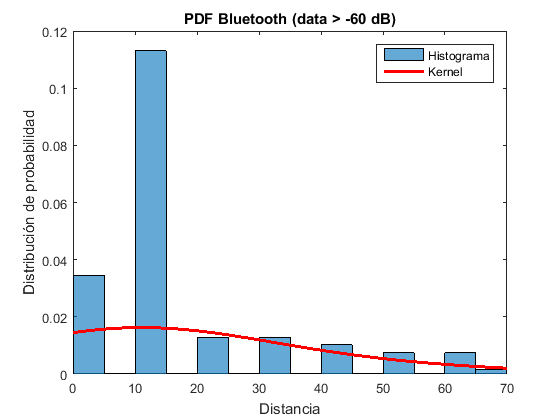
\includegraphics[width=0.5\textwidth]{images/histograma.png}
	\captionsetup{width=0.6\textwidth}
	\caption{Construcción de PDF por histograma comparado a la estimación Kernel. Gráfico producido en Matlab con las funciones $histogram$(values,`Normalization',`pdf') y $ksdensity$(values,0:70), respectivamente.}
    \label{fig:histograma}
\end{figure}

En la Figura \ref{fig:histograma} se construye el histograma de los valores de distancia obtenidos por experimentación para los cuales el RSS fue mayor a -60 dB ($D_{RSS>-60dB}$). Por lo tanto, dada un intensidad de señal por encima de -60 dB, la PDF indica con qué probabilidad se recibiría esa señal a una distancia dada respecto al monitor (ej. Dada una intensidad de señal $I=-55$ dB,  $p\approx0.04$ es la probabilidad de que haya sido transmitida desde las cercanías del detector). Frente a la estimación Kernel realizada sobre los mismos datos, se evidencia la naturaleza discreta del histograma. 

\begin{figure}[!htp]
	\centering
	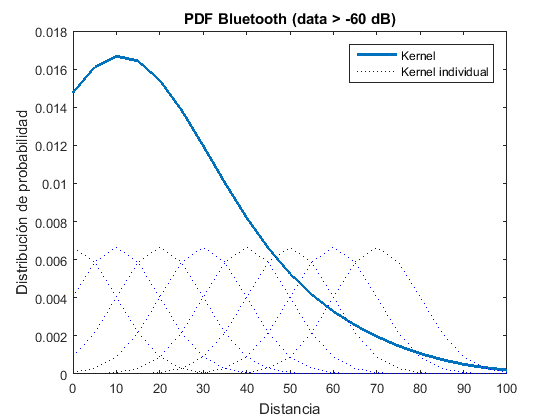
\includegraphics[scale=0.5]{images/kernel-individual.png}
	\captionsetup{width=0.7\textwidth}
	\caption{Estimación Kernel completa para el rango de señales mayores a -60 dB, junto con la estimación Kernel de cada valor, escaladas para la imagen.}
    \label{fig:kernel-individual}
\end{figure}

En la Figura \ref{fig:kernel-individual} se observa la misma estimación Kernel para el conjunto de valores muestreados $D_{RSS>-60}$. Las curvas punteadas pequeñas son las probabilidades de distribución para cada valor (kernels individuales). La curva mas alta es la distribución kernel completa. La función de suavizado Kernel se refiere a la forma de las curvas pequeñas, las cuales tienen una distribución normal en este ejemplo.
Existen otras opciones entre las cuales elegir la función de suavizado Kernel: Epanechnikov, triangular, rectangular, entre otras. 

Utilizando el total de las muestras, se observaron diferencias respecto al resultado esperado (\ref{fig:opdf-grouped} - All), donde paquetes con intensidad de señal alta predominan a distancias mayores. Para mejorar dichos resultados, además de extraer valores atípicos (Sección \ref{ssec:bt-simulation}), se agruparon las muestras en ventanas de $w=3$ y 5 paquetes (ver Apéndice), tomando la señal mínima, media y máxima de cada ventana. 

\begin{figure}[!htp]
	\centering
	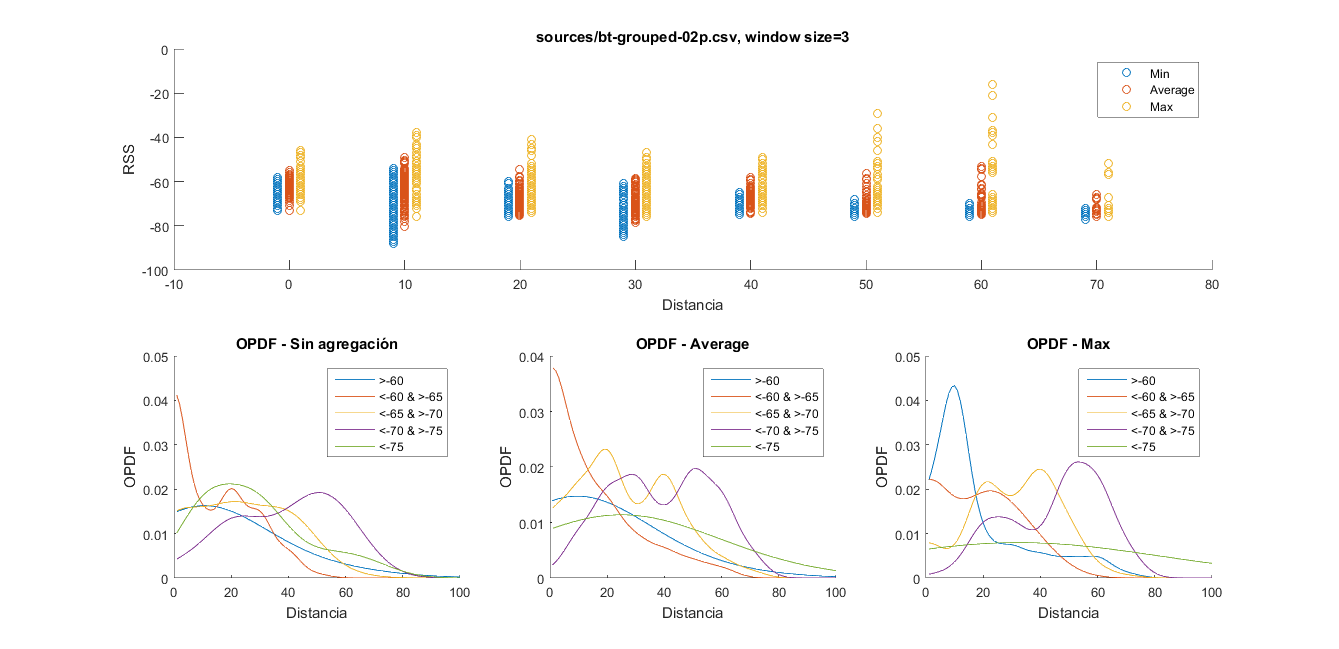
\includegraphics[width=\textwidth]{images/all_g-percentil=2-w=3.png}
	\captionsetup{width=0.9\textwidth}
	\caption{Arriba: Clasificación del dataset procesado con eliminación del 2\% de outliers (por cada grupo de distancia) y toma de valores mínimo, promedio y máximo en ventanas de 3 lecturas. Abajo: Funciones de densidad de probabilidades de observación para el mismo dataset, incluyendo todas las observaciones (All), el promedio (Average) y máximo (Max) de cada ventana.}
    \label{fig:opdf-grouped}
\end{figure}
 
 Entre las combinaciones posibles en cantidad de outliers removidos y tamaño de la ventana de agrupación, es deseable obtener la configuración que mejor represente el concepto de \textit{path loss} o pérdida de la intensidad de señal al propagarse por el espacio. En el espacio ideal (no obstruido y sin interferencias) se espera que la intensidad de señal decrezca al aumentar la distancia. Observando las estimaciones Kernel de las combinaciones planteadas se consideró más representativo el resultado de un porcentaje de eliminación de outliers $p_{outlier}=2$, tomando el máximo de  la agrupación de datos en ventanas de 3 elementos.

 Para la construcción de las OPDF en Java, se utilizó el componente \textit{KernelEstimator} de \textit{Weka}, una colección open-source de algoritmos de \textit{machine learning} para tareas de minería de datos. El paquete \textit{weka.estimators} contiene subclases de la clase genérica \textit{Estimator}, que calcula diferentes tipos de distribución de probabilidades. En este caso, para hacer la estimación Kernel se utilizó el componente \textit{KernelEstimator} del paquete \textit{weka.estimators}. 
 
 \begin{figure}[!htp]
	\centering
	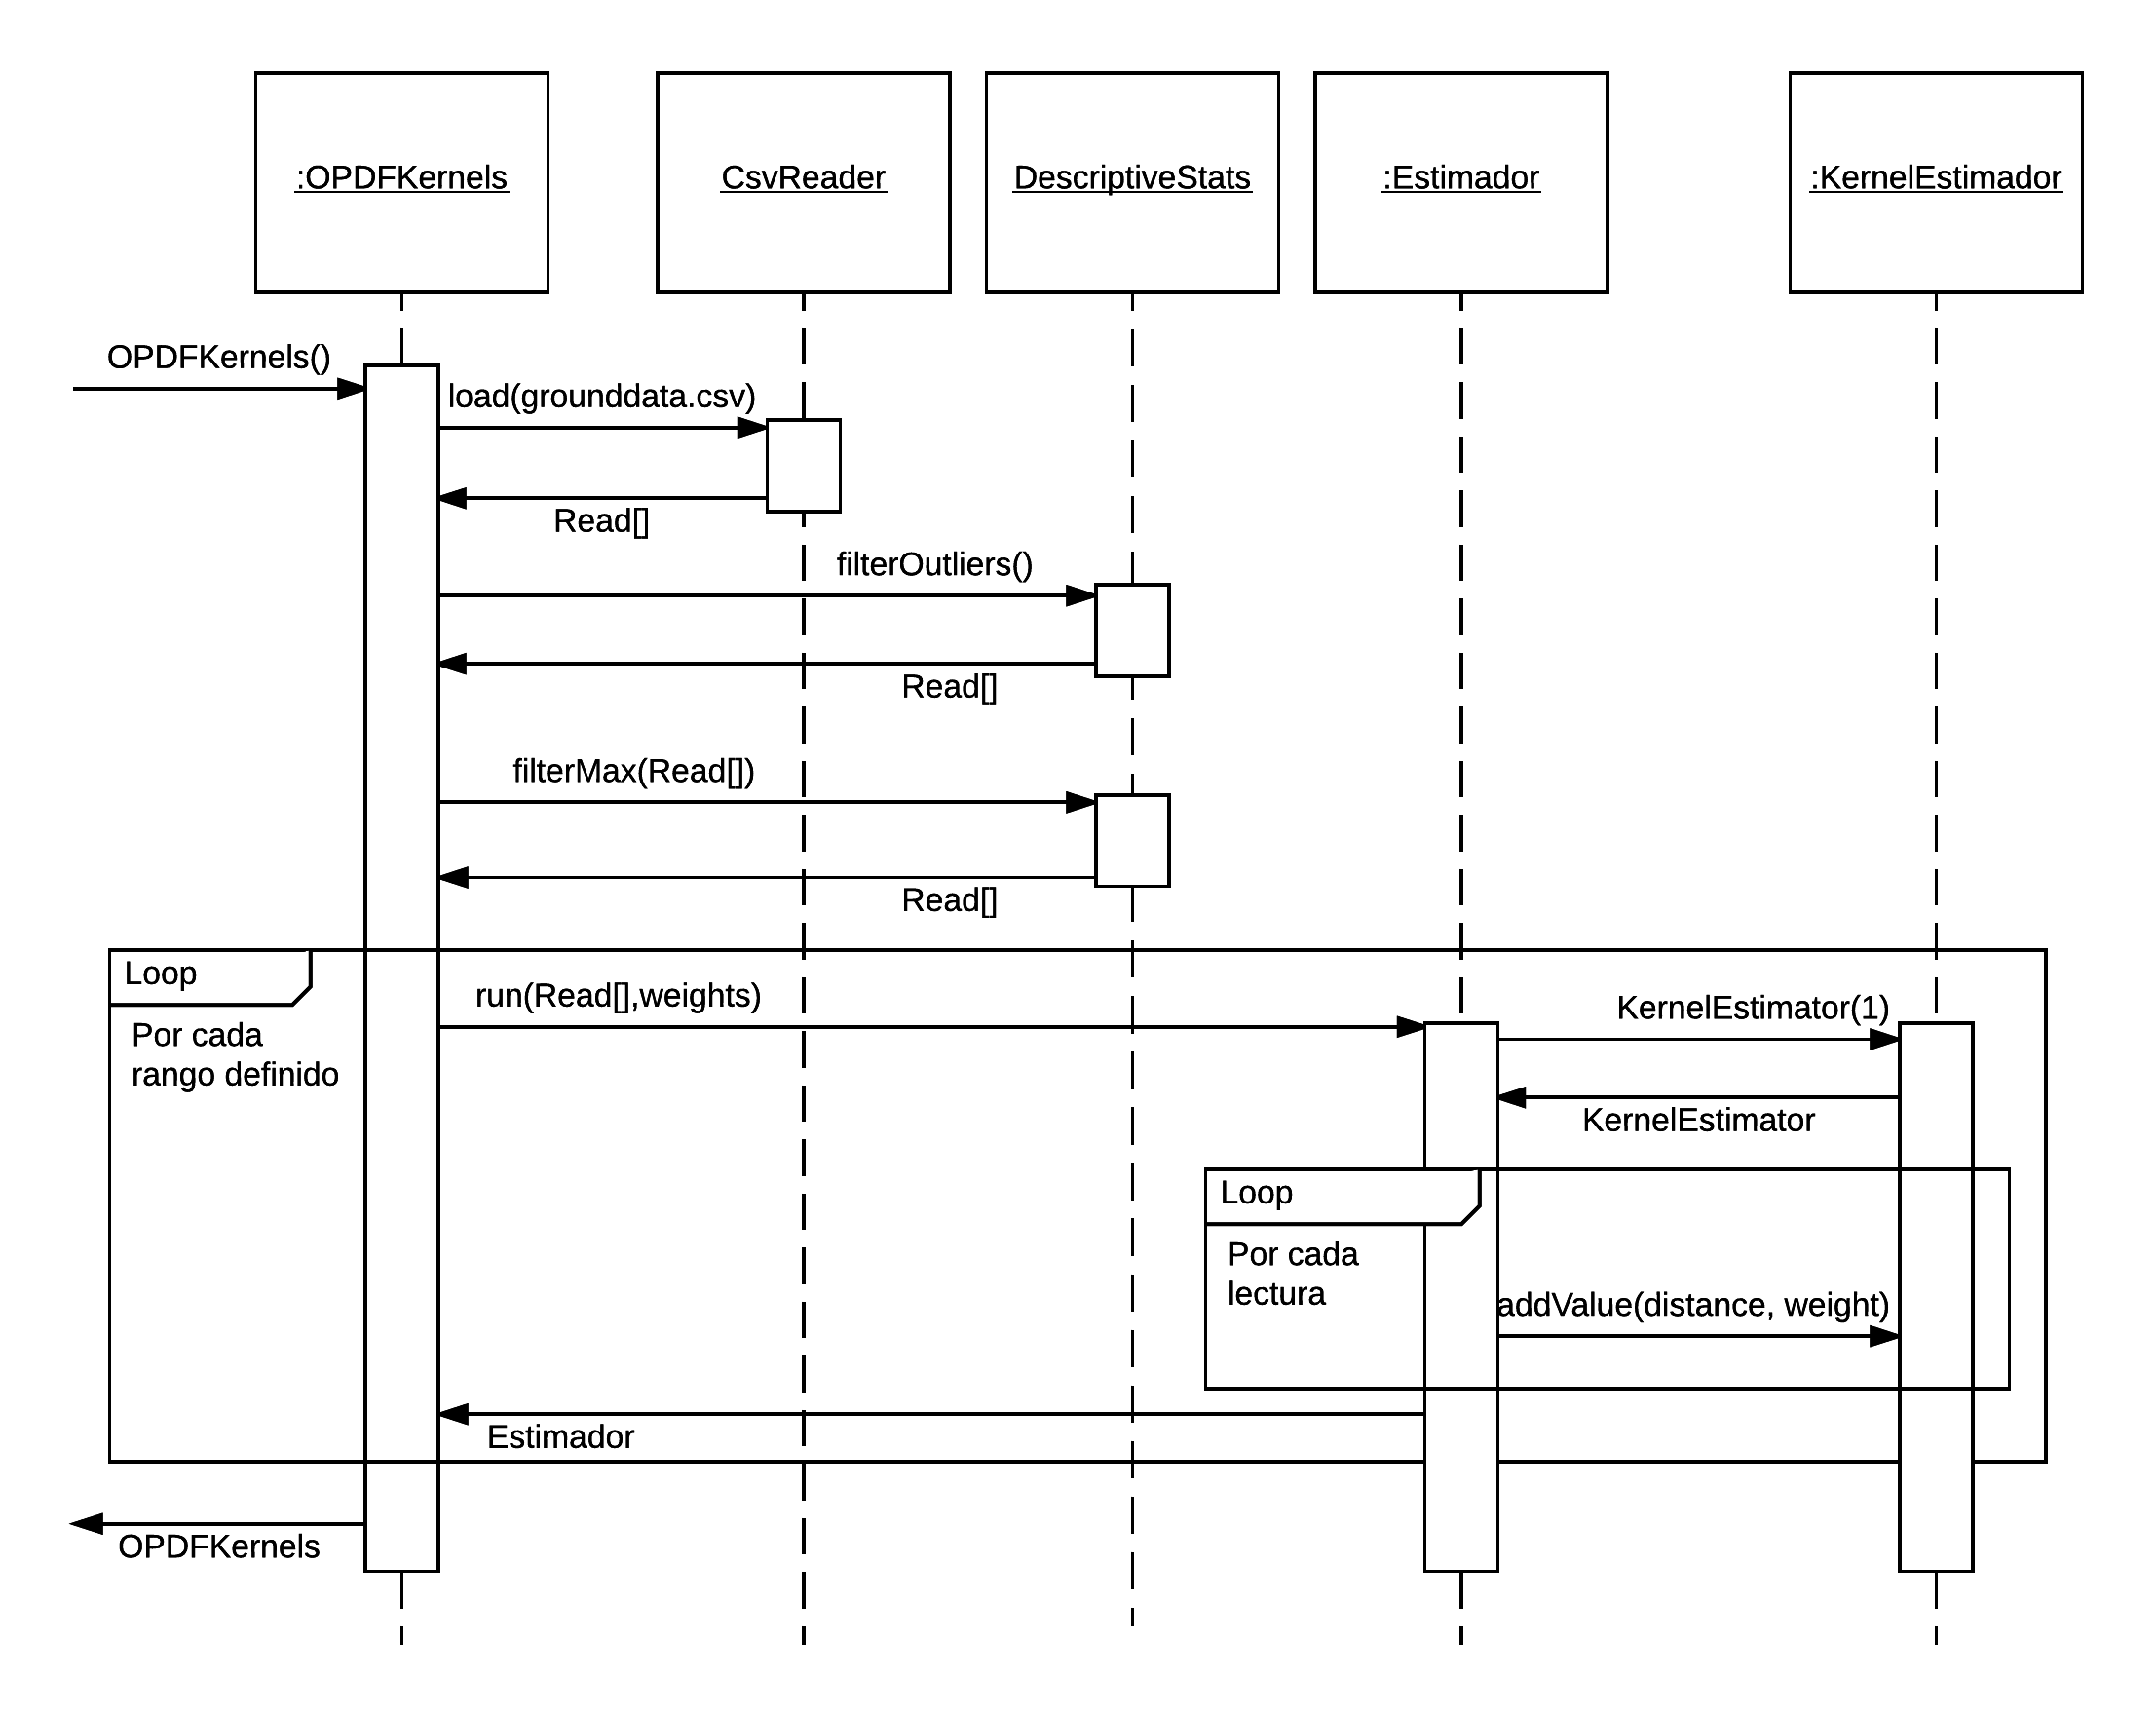
\includegraphics[width=0.9\textwidth]{images/sequence-opdfkernels.png}
	\captionsetup{width=0.9\textwidth}
	\caption{Diagrama de secuencia de la construcción de OPDFKernels.}
    \label{fig:sequence-opdfkernels}
\end{figure}

 El componente \textit{KernelEstimator} de \textit{Weka} se instancia con un parámetro de precisión. Este parámetro se utiliza para ajustar la precisión numérica los datos de entrada. Si se utiliza $precision=0.1$, los valores en el intervalo $[0.25, 0.35]$ serán tratados como 0.3. Los niveles de potencia de señal medidos tienen valores enteros por lo cual se usó $precision=1$. Para agregar datos al estimador, el componente define la interfaz $addValue(data,weight)$. El parámetro \textit{weight} es el peso asignado al dato y se utiliza para determinar el \textit{bandwith}.  
 
 Se construyen tantos estimadores \textit{KernelEstimator} como rangos de señal se hayan definido y se agrupan en el contenedor \textit{OPDFKernels}. Los datos de entrada para cada estimador son las distancias de las señales correspondientes a cada rango. 
 
 Finalmente, se obtiene $p(deteccion_m|s,tx)$ seleccionando un estimador a partir de la intensidad de señal observada (según el rango al que pertenece) y, desde el estimador, el valor de probabilidad, para una distancia dada $d$: $estimador.getProbability(d)$.

\subsection{Extensibilidad del módulo de estimación}

Las secciones anteriores describen las características funcionales de los paquetes principales \textit{org.tte.logic} y \textit{jahmm.extensions}. El primero, es un conjunto de elementos que dan soporte al procesamiento general de los mapas (carga, segmentación, instanciación del modelo \textit{Hmm} y construcción de OPDF). El segundo, naturalmente, contiene las implementaciones de \textit{Opdf} y extensiones de \textit{Observation}. 

En la Figura \ref{fig:modulos-logic} se observan las dependencias del paquete \textit{org.tte.logic} y cómo lo utilizan los componentes visuales en \textit{app.beans}. 

\begin{figure}[!htp]
	\centering
	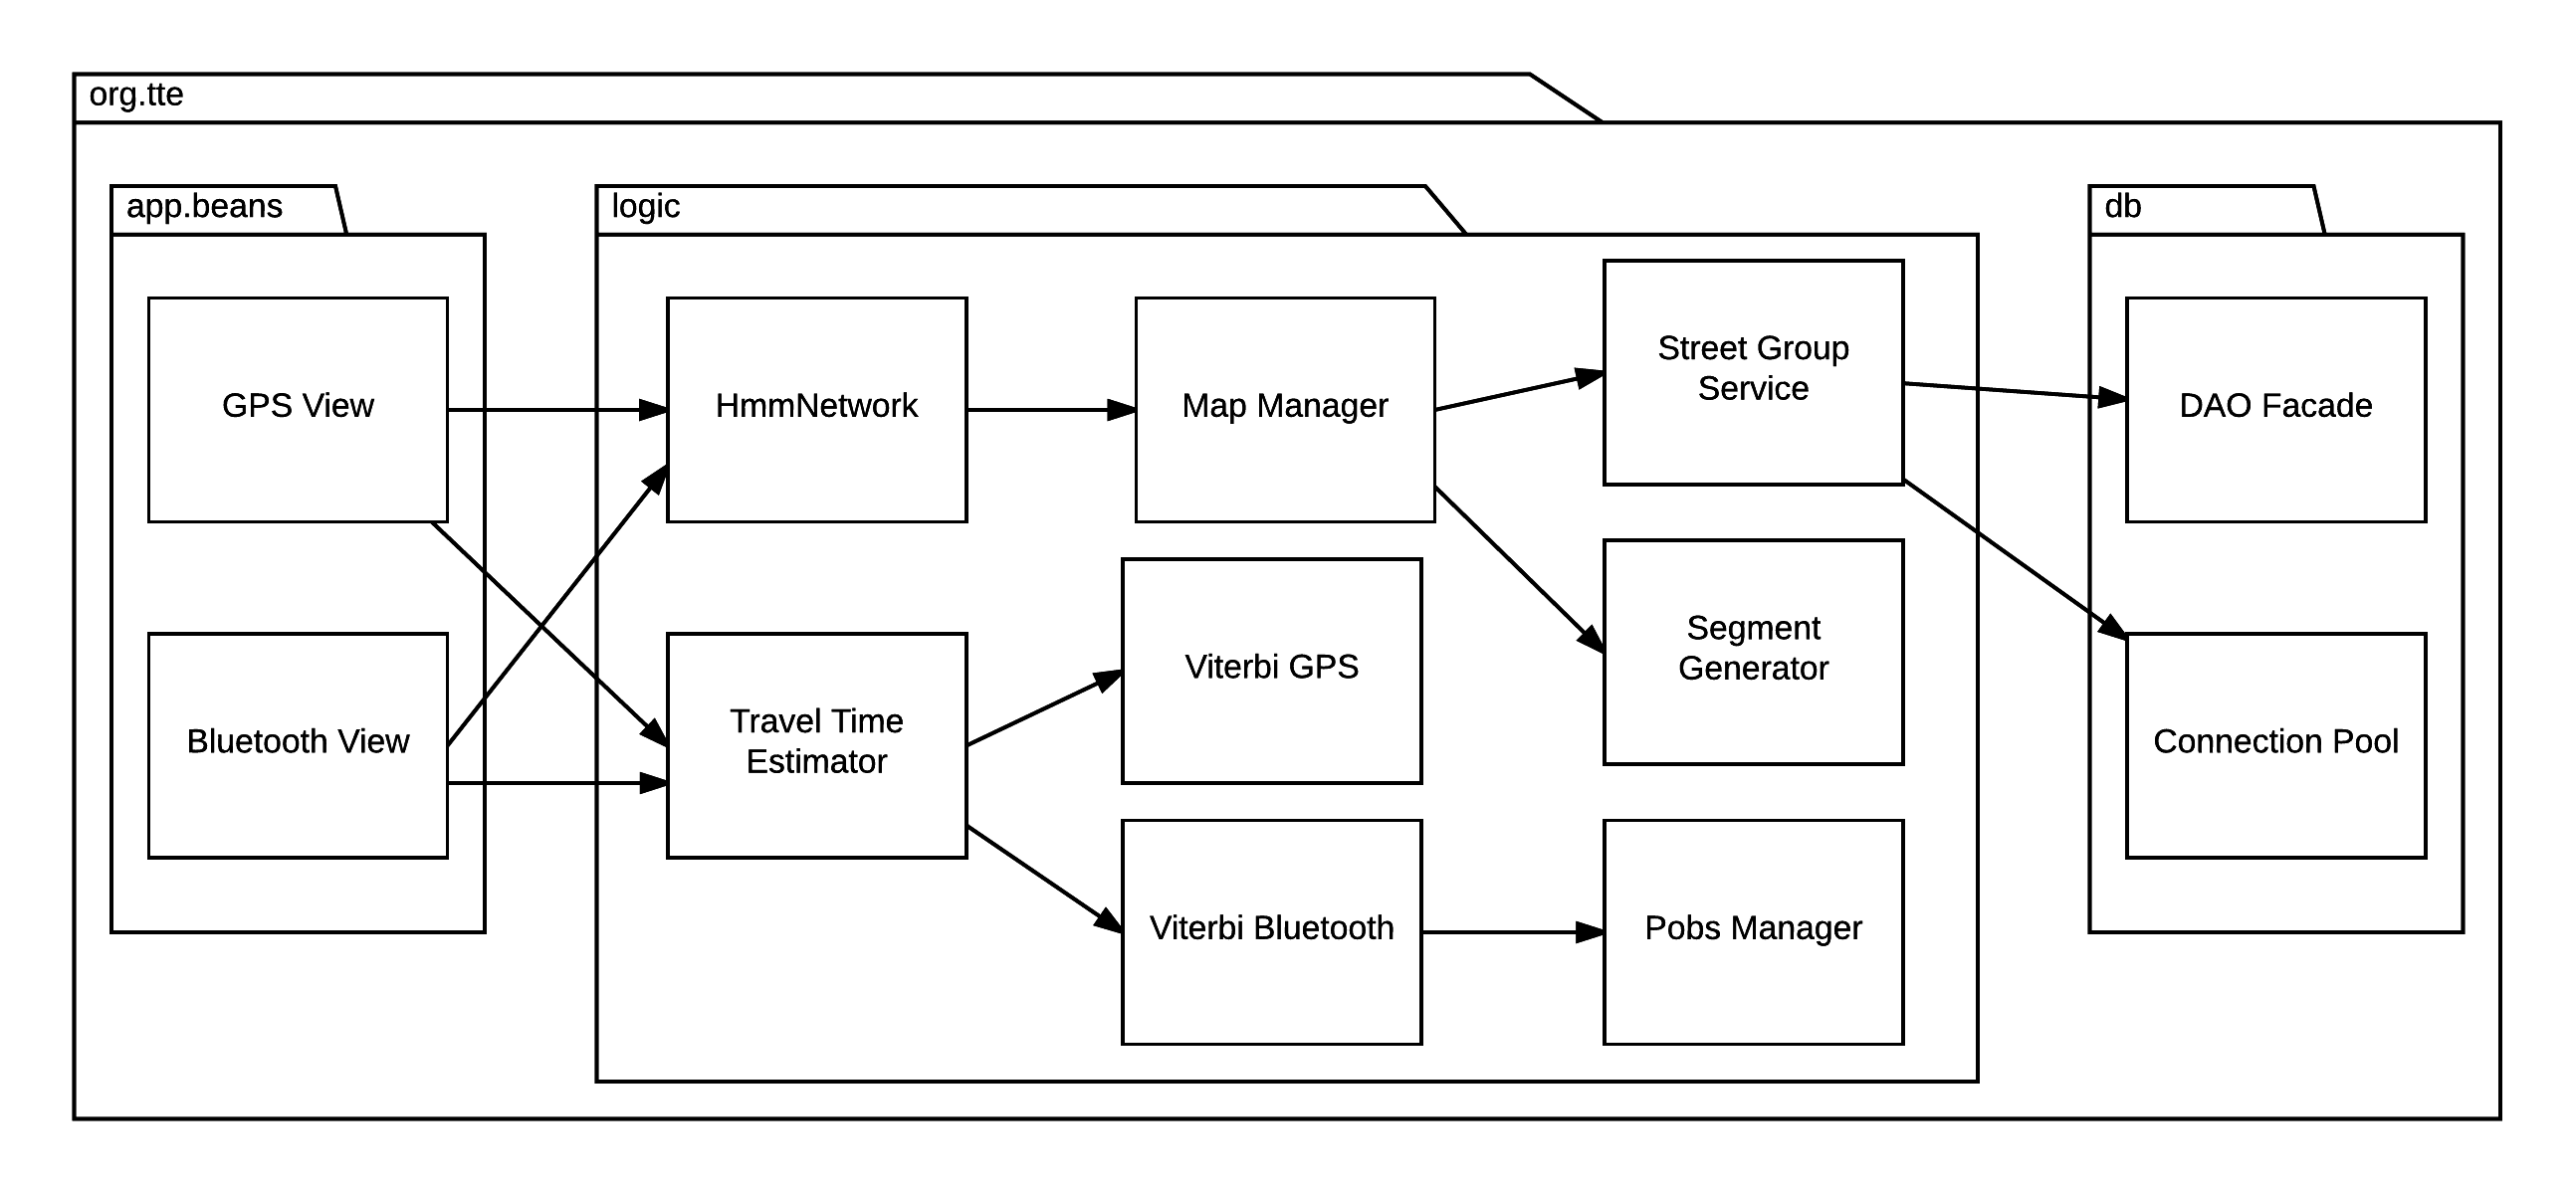
\includegraphics[width=0.9\textwidth]{images/modulos-logic.png}
	\captionsetup{width=0.9\textwidth}
	\caption{Clases de los paquetes \textit{org.tte.app.beans} y \textit{org.tte.logic} y \textit{org.tte.db}.}
    \label{fig:modulos-logic}
\end{figure}

Se demostró las posibilidad de extender la plataforma en la implementación de nuevos tipos de observaciones (\textit{ObservationEventVector}), como así también respecto a la extensión de las funciones de densidad de probabilidad como múltiples métodos de estimación. De este modo, para agregar un nuevo tipo de sensor, sólo se necesita utilizar la clase genérica \textit{Hmm<>} con el tipo de observación que más se ajuste a las necesidades del nuevo sensor y el método de estimación subyacente. En el caso de que las observaciones sean lo suficientemente complejas, se debe extender la clase \textit{Observation}. Adicionalmente, en el caso que las distribuciones de observación disponibles no sean aplicables, se deben construir las funciones de densidad de probabilidad de observación (OPDF) implementando la interfaz genérica \textit{Opdf<>}, utilizando como argumento de tipo una especialización de \textit{Observation}.

\subsection{Aritmética de punto flotante}

La utilización de HMM sobre secuencias de observaciones muy extensas conlleva el cálculo de probabilidades condicionales extremadamente pequeñas. Estas probabilidades introducen inestabilidad numérica en los cálculos requeridos para resolver los problemas definidos en la sección \ref{ssec:problemashmm}.

Cuando se implementan soluciones a estos problemas, se debe notar que muchos lenguajes utilizan aritmética de punto flotante. Como $p$ es pequeño, esto puede llevar a desbordamiento en los resultados. En el caso de secuencias de 100 000 observaciones o más, la probabilidad del camino óptimo será del orden de $10^{-100 000}$. La mayoría de los procesadores actuales se comportarían erroneamente con tales números.
Existen dos enfoques comunes que resuelven los conflictos al trabajar con probabilidades pequeñas. El primero, introducido por Rabiner \cite{rabiner1989tutorial}, consiste en escalar las probabilidades aplicando factores de escalado cuidadosamente diseñados. El otro enfoque es trabajar con los logaritmos de  probabilidades condicionales \cite{durbin1998biological}\cite{mann2006numerically}.

\subsubsection{Transformación logarítmica}

Para el algoritmo de Viterbi, siempre se debe utilizar el logaritmo de todas las probabilidades. Como el logaritmo de un producto es la suma de los logaritmos, todos los productos son convertidos en sumas. Asumiendo logaritmo en base 10, el logaritmo de la probabilidad $10^{-100 000}$ es -100 000. Así, el problema del desborde es resuelto. Además, la operación de suma es más veloz en algunos procesadores que el producto, acelerando el procesamiento en dichas computadoras.

Se muestra un tilde sobre los parámetros del modelo luego de tomar el logaritmo, de este modo se tiene por ejemplo $\tilde{a}_{ij} = \log a_{ij}$. Luego la variable de la recursión Viterbi (\ref{eqn:recursionviterbi}) se traduce a:
\begin{align}
    \Delta_{t+1}(j)=\tilde{b}_j(\mathrm{O}_{t+1})+\max_i\{\Delta_t(i)+\tilde{a}_{ij}\} 
\end{align}

donde $\Delta$ es el logaritmo de $\delta$.

Es mas eficiente tomar el logaritmo de todos los parámetros del modelo antes de ejecutar el algoritmo de Viterbi, para evitar aplicar la función logaritmo repetidamente durante las iteraciones.


\section{Visualizador}
Para la visualización de resultados se desarrolló una aplicación Web en la plataforma Java EE (Enterprise Edition). Entre las herramientas disponibles, se utilizó la biblioteca de componentes open-source Primefaces para JavaServer Faces (JSF). Esta biblioteca ofrece una gran variedad de componentes visuales que facilitan la creación de aplicaciones Web. La arquitectura predefinida por el framework establece la separación del código en capas, en particular se utiliza el patrón Model-View-Controller (MVC) para la separación de responsabilidades entre visualización y lógica de negocio. Aquí se hace la salvedad de enmarcar la lógica de negocio y el acceso a datos en la capa \textit{Model} (``Modelo''), para simplificar la representación visual. 

El patrón MVC surge como diseño recurrente en implementaciones de interfaces de usuarios (UI) en los comienzos de la computación gráfica. La capa \textit{View} (Vista) contiene la implementación de interfaces visuales y el \textit{Model}  la representación del modelo de datos. Originalmente, se definió la comunicación de las capas de modo que el Controlador es quién se comunica con el Modelo para obtener datos y redirigirlos a la Vista.

\begin{figure}[!htp]
	\centering
	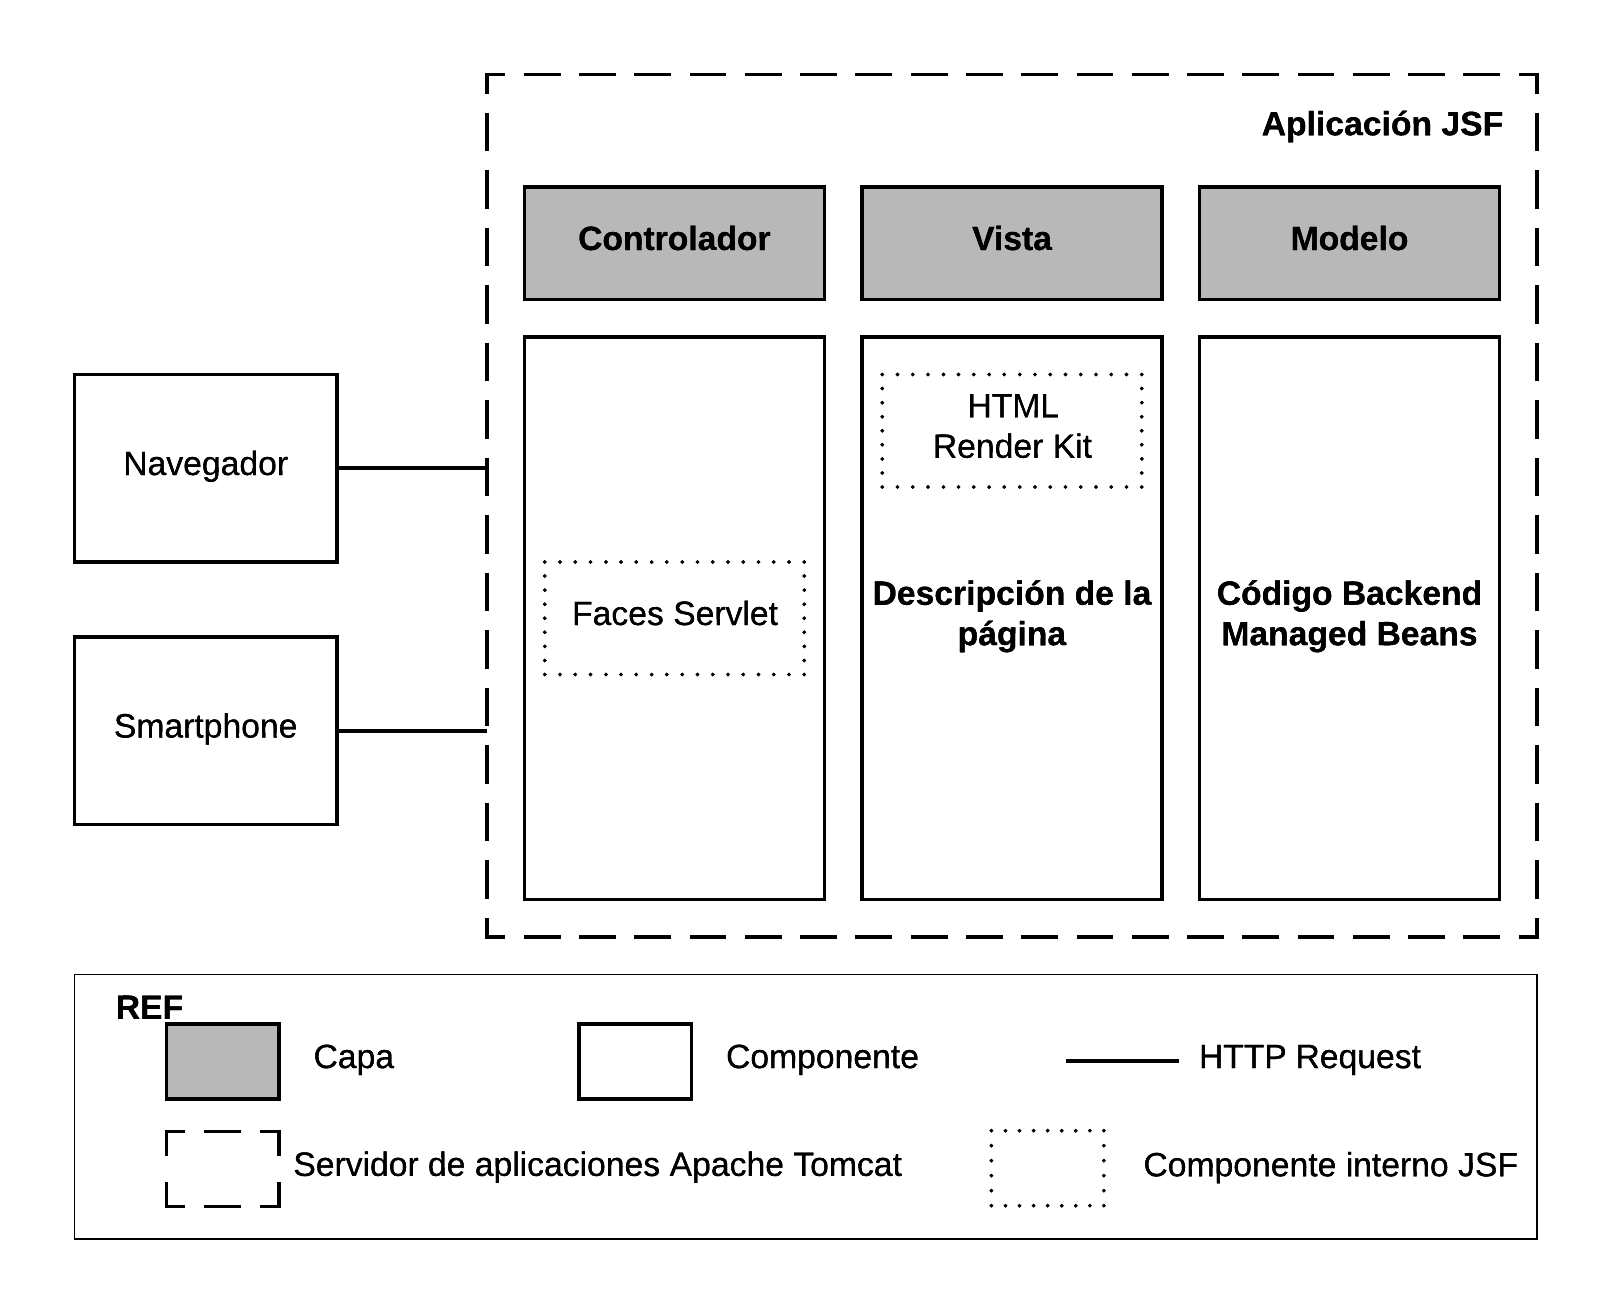
\includegraphics[width=0.9\textwidth]{images/mvc-jsf.png}
	\captionsetup{width=0.9\textwidth}
	\caption{Vista de módulos de una aplicación JavaServer Faces.}
    \label{fig:mvc-jsf}
\end{figure}

 Algunas modificaciones proponen que la Vista consulte directamente al Modelo o incluso, que el Modelo sea quién actualice la vista. En el caso de Primefaces, predomina el uso del patrón en su forma original. Implementaciones nuevas de la biblioteca (actualmente se encuentra en la versión 5) ofrecen mecanismos PUSH para la actualización de la vista desde el servidor. La Figura \ref{fig:mvc-jsf} ilustra la comunicación entre capas para aplicaciones JSF.
 
 En JSF se introducen los conceptos de ``Managed Beans'', estos son componentes que se comunican con la lógica de la aplicación. Se pueden definir en un archivo de configuración \textit{faces-config.xml} o a través de anotaciones (@ManagedBean). Una vez definidos se pueden usar en todo el contexto de la aplicación.
 
 La capa \textit{View} de JSF describe la distribución, comportamiento y rendering de la aplicación. Uno de los pilares de JSF es el \textit{UIComponent}. A través de la colocación de \textit{UIComponents} se representa la estructura y comportamiento de los elementos en una página.
 
 Por otro lado, la capa \textit{Controller} simplemente incluye el componente \textit{FacesServlet} que actúa como manejador de peticiones, controlando el flujo de navegación y la redirección de solicitudes a las páginas JSF correspondientes.
 
 Algunos de los componentes de Primefaces utilizados en este trabajo son:
 
 \begin{itemize}
    \item Panel (Contenedores HTML)
    \item Button (Botones con manejadores de eventos asociados)
    \item DataTable (Tablas mapeadas a objetos del dominio.)
    \item Charts (Gráficos de barra y línea)
    \item Growl (Notificaciones sobre la pantalla)
    \item File Upload (Transferencia de archivos al servidor)
 \end{itemize}
 
 Para visualizar mapas se evaluaron distintas tecnologías: Google Maps, Leaflet y MapBox. Finalmente, se seleccionó Leaflet por soportar mapas OpenStreetMap y por su facilidad de uso. Sólo requiere un token de acceso que se obtiene desde la página oficial y en pocas líneas es posible mostrar un mapa simple con características agregadas (marcadores, formas geométricas, etc). En el extracto de código \ref{alg:leaflet} se ejemplifica la configuración necesaria para mostrar un mapa básico.
 
 \begin{lstlisting}[language=Html, caption=Configuración de la visualización de mapas, label=alg:leaflet]
<!DOCTYPE html>
<html>
<head>
	<link rel="stylesheet" href="http://cdn.leafletjs.com/leaflet/v0.7.7/leaflet.css" />
</head>
<body>
	<div id="mapid" style="width: 600px; height: 400px"></div>
	<script src="http://cdn.leafletjs.com/leaflet/v0.7.7/leaflet.js"></script>
	<script>
		var mymap = L.map('mapid').setView([51.505, -0.09], 13);

    L.tileLayer('https://api.tiles.mapbox.com/v4/{id}/{z}/{x}/{y}.png?access_token={accessToken}', {
    maxZoom: 18,
    id: 'mapbox.project.id',
    accessToken: 'mapbox.public.access.token'
}).addTo(mymap);
	</script>
</body>
</html>
\end{lstlisting}

La mayoría de los motores de mapas soportan el reciente estándar ``GeoJSON'' (basado en texto plano) para la representación de elementos georreferenciados. A través de una interfaz muy sencilla (Algoritmo \ref{alg:leaflet-geojson}) se pueden agregar capas (superpuestas al mapa base) con características agregadas.

\clearpage

\begin{lstlisting}[language=Html, caption=Carga de una representación GeoJSON en Leaflet, label=alg:leaflet-geojson]
var geojsonFeature = {Objeto GeoJSON}
L.geoJson(geojsonFeature).addTo(map);
\end{lstlisting}

El mapa de la red y el resultado de las estimaciones de tiempo de viaje se visualizan con rectángulos formando los segmentos \textit{SegmentoViterbi}. Los Monitores Bluetooth y las observaciones GPS son representadas por puntos (círculos) de diferentes colores (Figura \ref{fig:captura-viterbi-gps}).


\begin{figure}[!htp]
	\centering
	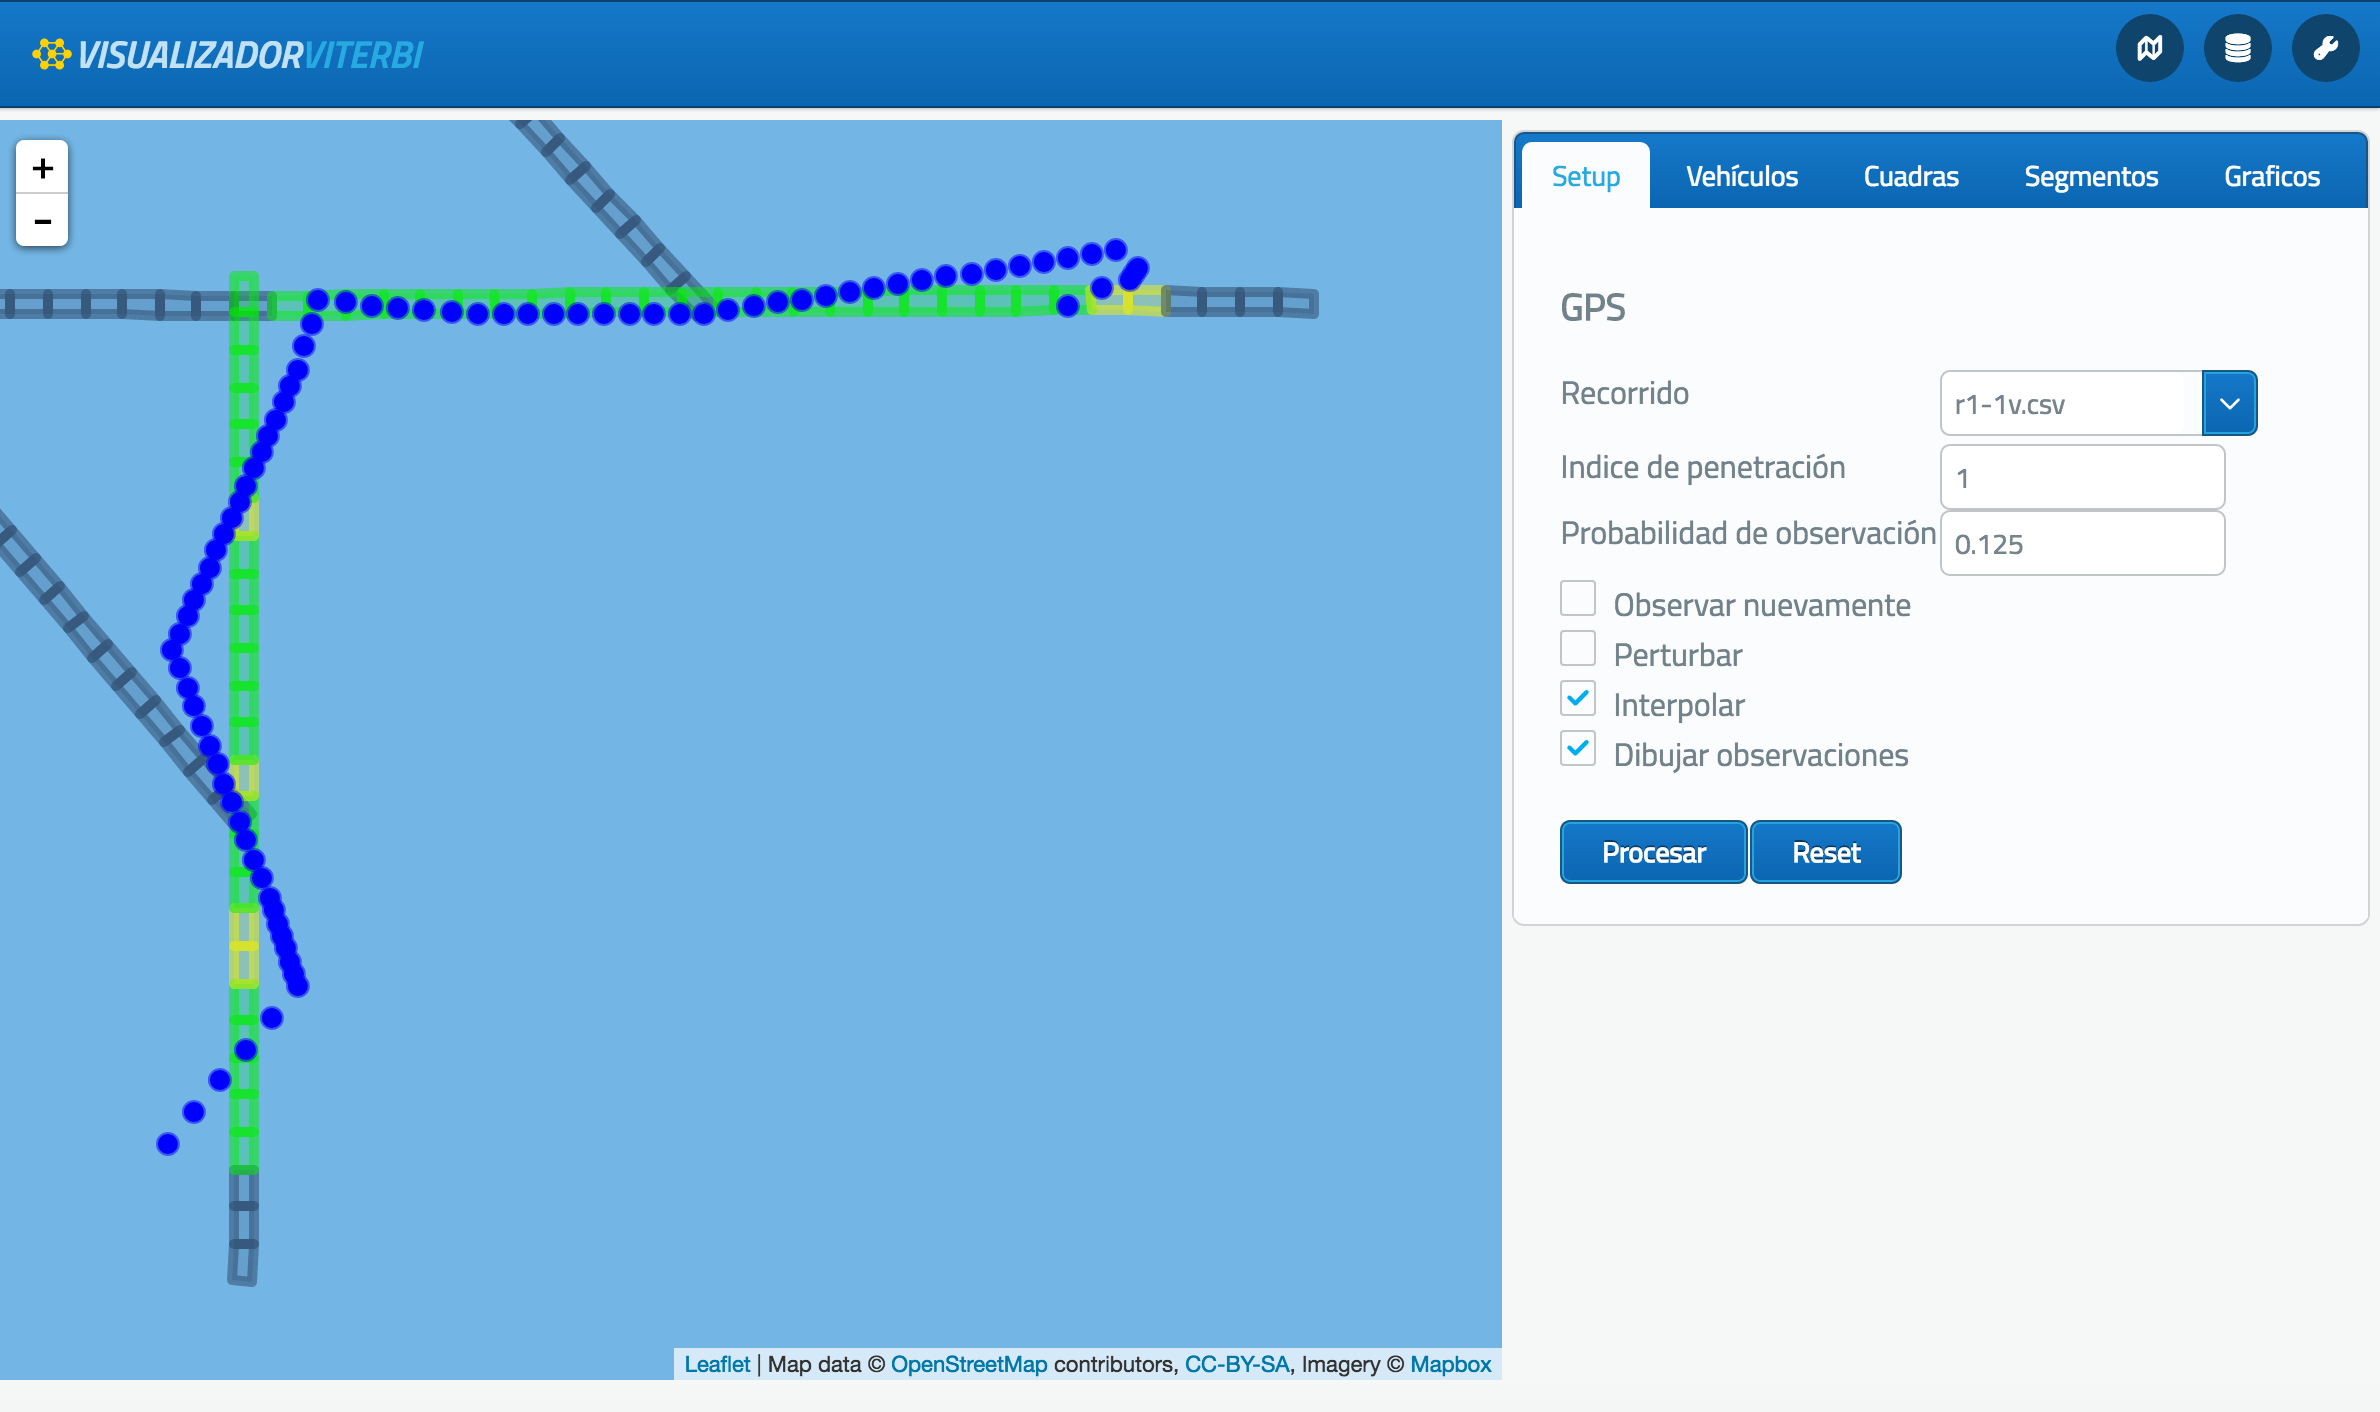
\includegraphics[width=0.8\textwidth]{images/captura-viterbi-gps.png}
	\captionsetup{width=0.7\textwidth}
	\caption{Captura de pantalla del estimador GPS}
    \label{fig:captura-viterbi-gps}
\end{figure}

Se incorporan los siguientes parámetros de ajuste a las estimaciones GPS y Bluetooth:

\begin{description}
    \item[Recorrido:] Recorrido seleccionado (pre-cargado).
    \item[Índice de penetración:] Es el porcentaje de vehículos que serán ``observados'' del total de cada recorrido.
    \item[Probabilidad de lectura:] Es el porcentaje de observaciones que se tomarán (aleatoriamente) de cada vehículo, sobre el total de la muestras de cada uno en el recorrido.
\end{description}

Para las observaciones GPS se aplican, además, otros ajustes:

\begin{description}
    \item[Observar Nuevamente:] Realiza el proceso de carga aplicando como filtro la probabilidad de penetración y de lectura indicados.
    \item[Perturbar:] Aplica una perturbación aleatoria a cada observación basada en una distribución normal bivarada con media 0 y un desvío dado en metros.
\end{description}
 
 \subsection{Procesador GeoJSON}
 Para generar la especificación en formato GeoJSON se implementó un componente especial, separado del resto de la aplicación en forma de biblioteca, llamado \textit{Java2GeoJSON}. Se utiliza para traducir los objetos del dominio a una representación GeoJSON válida. Esta herramienta se aplica sobre las estructuras internas (\textit{SegmentoViterbi}, \textit{AccessPoint} y \textit{List<ObservationSimple>}) desde los \textit{ManagedBean} que administran las páginas de estimación.
 
 GeoJSON es un formato para codificar una gran variedad de estructuras de datos geograficos, basado en JavaScript Object Notation (JSON). 
Es ligero y está formulado en lenguaje natural sencillo, lo cual lo convierte en una herramienta ideal para uso compartido y colaborativo. El estándar fue presentado en el año 2014 en el grupo IETF y al día de la fecha se encuentra como documento activo. Se recomienda utilizar un único sistema de coordenadas de referencia basado en WGS 84.

Soporta los siguientes tipos de geometrías: Punto, Línea, Polígono, MultiPunto, MultiLínea y MultiPolígono. Elementos geométricos con propiedades adicionales son los objetos \textbf{Feature}. Un conjunto de objetos \textit{Feature} es contenido por objetos
\textbf{FeatureCollection}.

Tras su presentación como estándar, GeoJSON se convirtió en un formato ampliamente soportado por los motores de mapas disponibles en la red.

La biblioteca \textit{Java2GeoJSON} está desarrollada en el lenguaje Java para integrarse a los desarrollos existentes. Permite codificar figuras en GeoJSON a partir de los elementos del dominio que ya existen en una aplicación. 

A modo de ejemplo, en el código \ref{code:buildFeature} se crea una polilínea (Figura \ref{fig:polyline}) formada a partir de una secuencia de puntos de ejemplo (\textit{path}). La secuencia de puntos originalmente está representada como una secuencia de Nodos, los cuales poseen el par de referencia \textit{latitud,longitud}. Para la traducción (o codificación) se recorre la estructura existente y se forma la capa de figuras (\textit{GeoFeature}) agregando nodos en el objeto \textit{polyline}.

\begin{lstlisting}[caption={Código para la creación de una capa},captionpos=b,label={code:buildFeature},frame=single]  % Start your code-block

GeoFeature[] parsePath(Node[] path){
    //Generate GeoJson objects
    GeoFeature pathLayer = new GeoFeature();
    GeoPolyline polyline = new GeoPolyline();       
    for (Node node : path) {                        
        float lat = node.getLat();
        float lng = node.getLng();
        polyline.addCoordinate(lat, lng);                                   
    }
    pathLayer.setGeometry(polyline);
    return new GeoFeature[]{pathLayer};
}\end{lstlisting}


\begin{figure}[!ht]
  \centering
	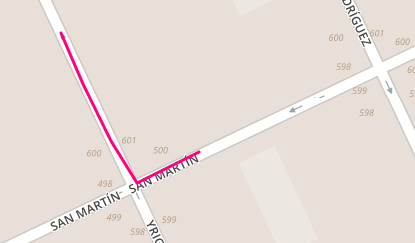
\includegraphics[width=0.6\textwidth]{images/polyline.png}%
    \caption{\label{fig:polyline}Resultado gráfico de la codificación de una secuencia de puntos de ejemplo.}
\end{figure}

Además de la definición de geometrías, es posible añadir propiedades adicionales a cada elemento o \textit{Feature}. Es posible llevar anotaciones, como identificadores de figuras o realizar configuraciones de colores y bordes de cada figura en particular. El funcionamiento de estas últimas configuraciones dependen de la implementación de la herramienta de visualización, ya que la definición de propiedades de colores y bordes de \textit{Features} no está contemplada por el estándar.

\begin{lstlisting}[caption={Código para configurar propiedades adicionales},captionpos=b,label={code:properties},frame=single]  % Start your code-block

feature.addProperty("id", "Linea 1");
feature.addProperty("fill", "#ffffff");
feature.addProperty("fill-opacity", "1");
\end{lstlisting}

\section{Módulo Monitores.WS}

Para procesar las detecciones obtenidas desde las diferentes herramientas de captura, es necesario que estas sean transmitidas al servidor central. El objetivo de éste módulo es proveer interfaces (\textit{endpoints}) de almacenamiento para los distintos tipos de detecciones, vía servicios web. Para aumentar la interoperabilidad, se construyeron dos APIs (Application Programming Interface) para agregar, modificar o eliminar detecciones. Estas API se han implementado siguiendo los esquemas:

\begin{itemize}
\item REST (Representational State Transfer)
\item SOAP (Simple object Access Protocol)
\end{itemize}

Estas son dos especificaciones distintas para la implementación de servicios web. En muchos lenguajes, como Java o C\#, existen herramientas que facilitan el desarrollo de clientes para estas API.

\begin{figure}[!htp]
	\centering
	\frame{
	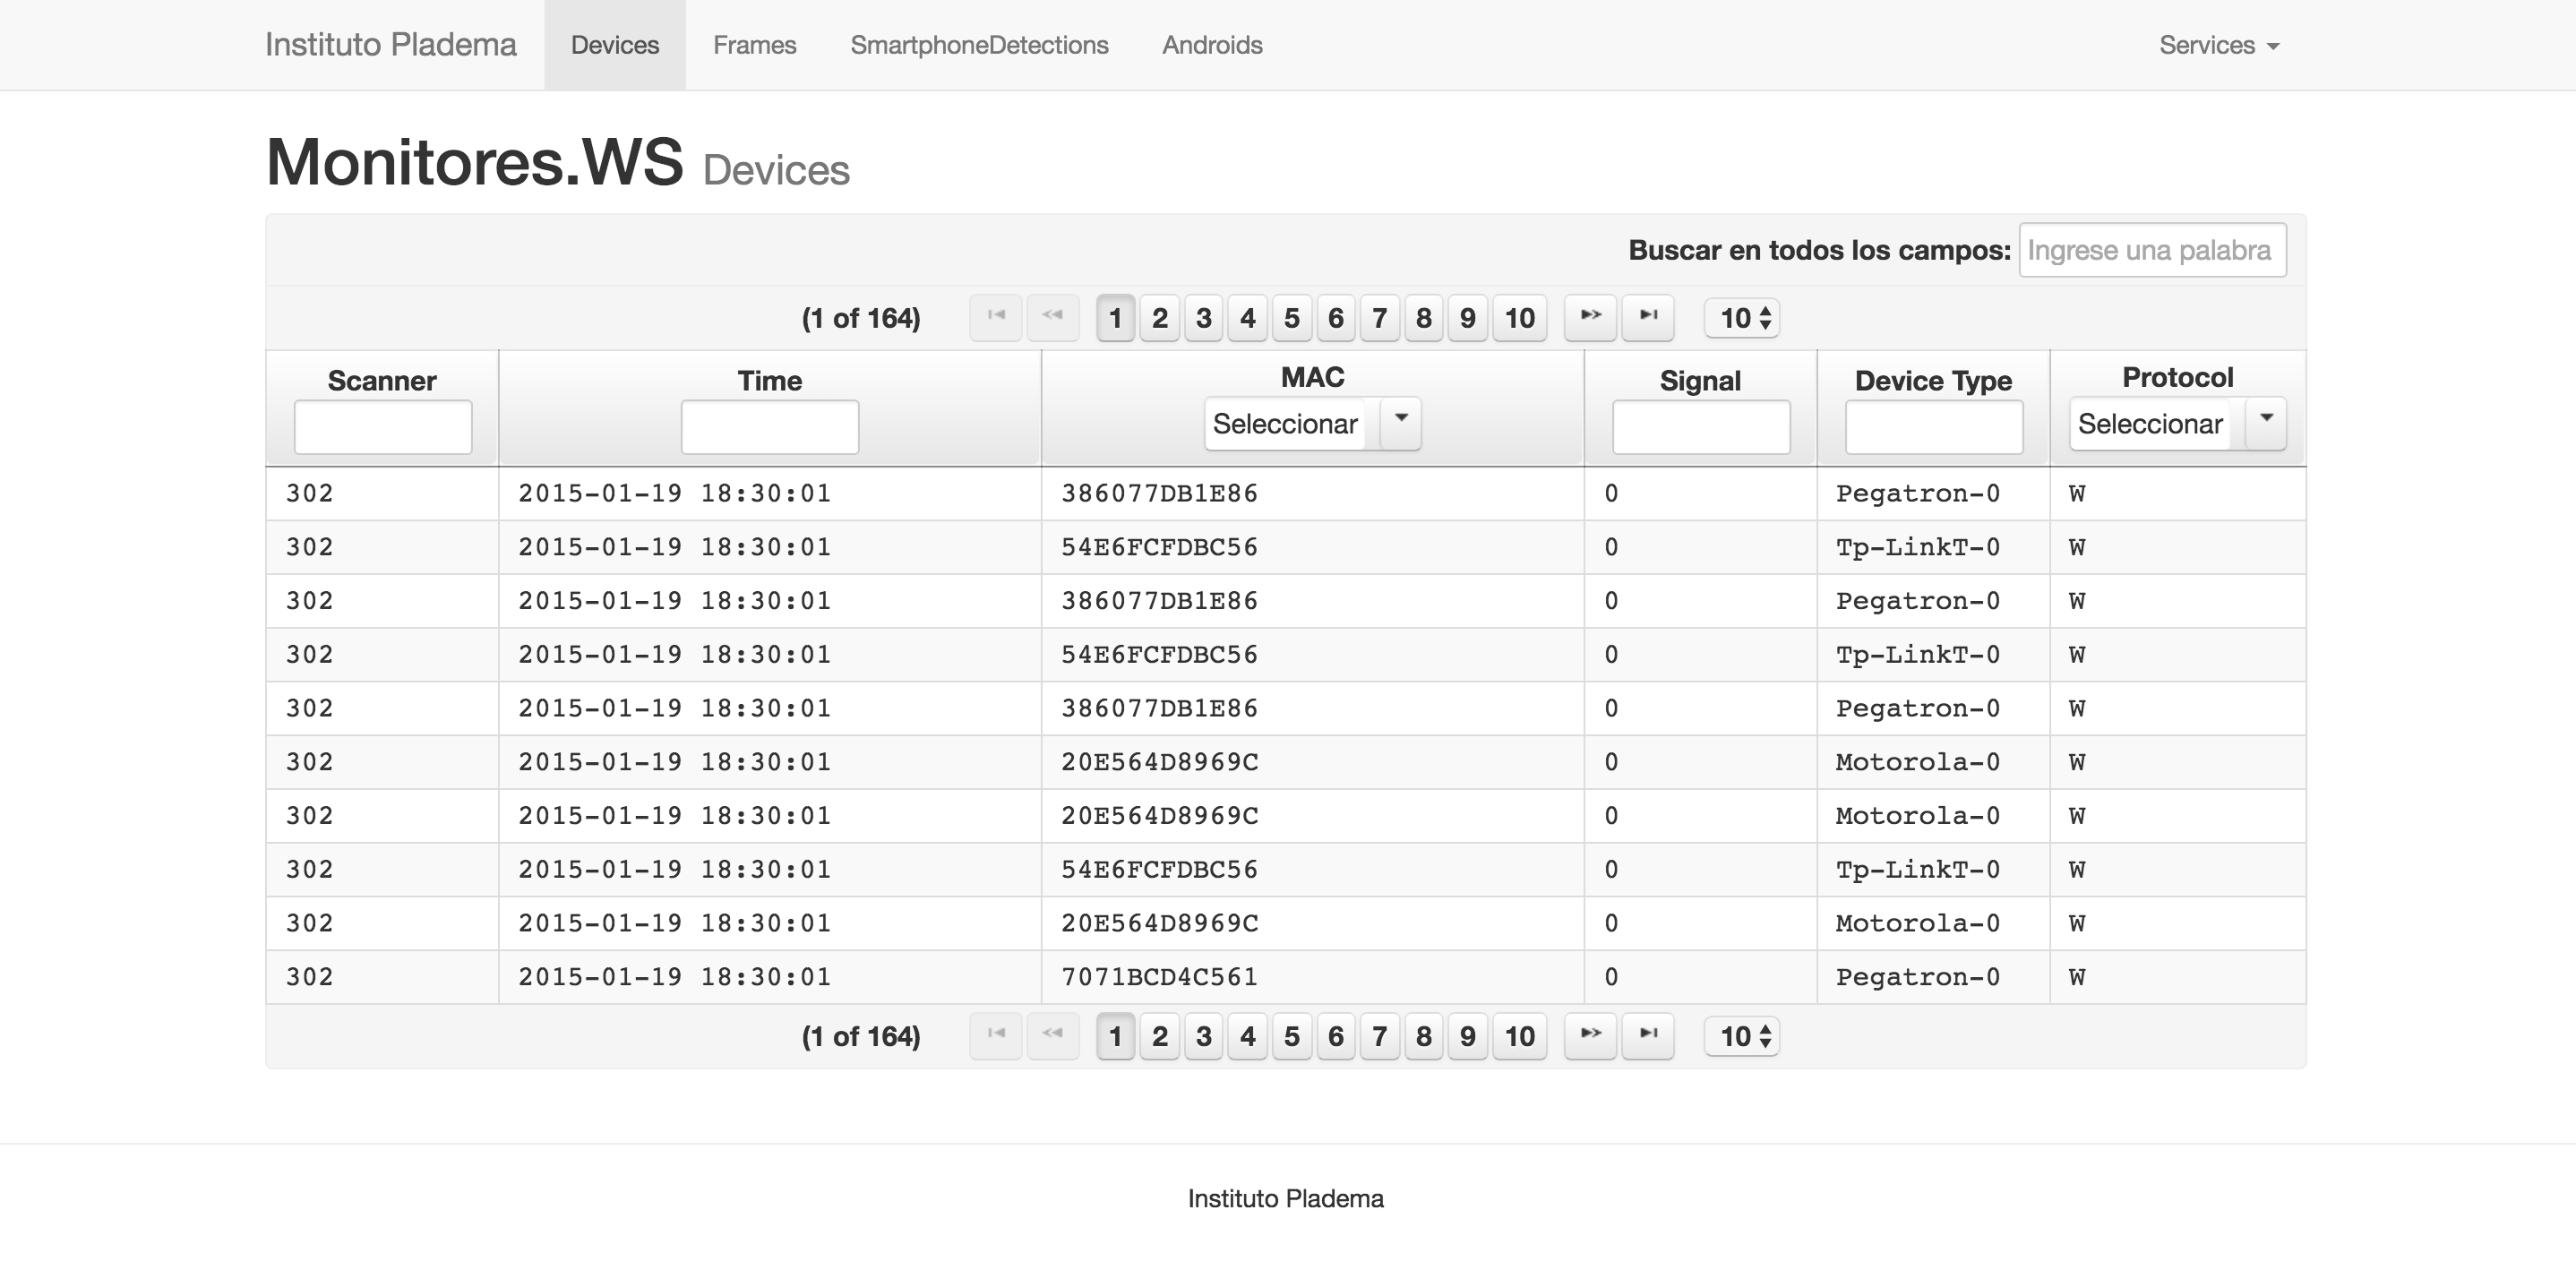
\includegraphics[width=0.9\textwidth]{images/screen-monitoresws.png}}
	\captionsetup{width=0.9\textwidth}
	\caption{Captura de imagen del sitio Web de Monitores.WS}
    \label{fig:monitoresws}
\end{figure}

A través de una página web se pueden visualizar y filtrar los datos cargados (Figura \ref{fig:monitoresws}). Las páginas fueron desarrolladas con la misma tecnología de visualización que el módulo \textit{Viterbi} (usando la combinación de herramientas \textit{Primefaces} y \textit{Hibernate}).

La implementación de los web services se realiza con el framework \textit{Spring Boot} y los submódulos \textit{Spring Boot Data Rest} y \textit{Spring Boot Starter WS}, para las implementaciones REST y SOAP, respectivamente. Se definen \textit{endpoints} para los siguientes recursos:

\begin{itemize}
\item Monitores/Detectores
\item Smartphone Detections
\item Bluetooth Detections
\item Video detections
\end{itemize}

Los \textit{tests} durante el desarrollo de los web services se realizaron con la herramienta POSTMAN, una herramienta web para construir suites de \textit{testing} para endpoints REST y SOAP (vía HTTP). POSTMAN permite configurar todos los parámetros de las solicitudes HTTP. 

